\PassOptionsToPackage{usenames,dvipsnames}{xcolor}

\documentclass[amsmath,table,amsfonts,hyperref={colorlinks,citecolor=blue,linkcolor=blue,urlcolor=applegreen}]{beamer}

\usepackage{tikz}
\usetikzlibrary{calc,decorations.pathreplacing,decorations.markings,positioning,shapes}

\usepackage{graphicx}
\usepackage{pgf}

\definecolor{applegreen}{rgb}{0.55, 0.71, 0.0}

\usepackage{fourier-orns}  %fancy symbols https://mirror.easyname.at/ctan/fonts/fourier-GUT/doc/fourier-orns-doc.pdf

\usepackage{mathbbol} %%%% for \mathds{1}

%%%%%%%%%%%%%%%%%%%%%%%%%%%%%
\usepackage{iftex}
\ifxetex
%
% XeLaTeX
%
\XeTeXinputencoding "cp1252"

\usepackage{fontspec}
\setmainfont{Garamond}
\setsansfont{Garamond}

\else
\usepackage[latin1]{inputenc}
\usepackage[T1]{fontenc}
\fi
%%%%%%%%%%%%%%%%%%%%%%%%%%%%%

\beamertemplatetriangleitem

\beamerboxesdeclarecolorscheme{alert}{red}{red!15!averagebackgroundcolor}

\setcounter{MaxMatrixCols}{20}

\begin{document}

\title{\bf \textcolor{blue}{``How-to'' systematically compute probabilistic costraints such as optimal Boole-Bell type inequalities by assessing extreme situations}}
\subtitle{\scriptsize{\url{http://tph.tuwien.ac.at/~svozil/publ/2020-b-pres.pdf}}
}
\author{Karl Svozil}
\institute{ITP TU Wien, Vienna Austria\\
svozil@tuwien.ac.at
%{\tiny Disclaimer: Die hier vertretenen Meinungen des Autors verstehen sich als Diskussionsbeitr�ge und decken sich nicht notwendigerweise mit den Positionen der Technischen Universit�t Wien oder deren Vertreter.}
}
\date{Online presentation, summer of 2021}
\maketitle


%%%%%%%%%%%%%%%%%%%%%%%%%%%%%%%%%%%%%%%%%%%%%%%%%%%%%%%%%%%%%%%%%%%%%%%%%%%%%%%%%%%%%%%%%%%%%%%%%%%%%%%%%%%%%%%%%%
%
%\begin{frame}
%\frametitle{Contents}
%\tableofcontents
%\end{frame}
%
%%%%%%%%%%%%%%%%%%%%%%%%%%%%%%%%%%%%%%%%%%%%%%%%%%%%%%%%%%%%%%%%%%%%%%%%%%%%%%%%%%%%%%%%%%%%%%%%%%%%%%%%%%%%%%%%%%

%\input 2020-b-pres-start.tex


\section{The big picture---Strategies {\&} \textbf{tactical moves}}

\subsection{Strategy}
%%%%%%%%%%%%%%%%%%%%%%%%%%%%%%%%%%%%%%%%%%%%%%%%%%%%%%%%%%%%%%%%%%%%%%%%%%%%%%%%%%%%%%%%%%%%%%%%%%%%%%%%%%%%%%%%%%

\begin{frame}
\begin{center}
{\large {\color{purple}$\;$}}
\end{center}

                                                    \vspace{1.15cm}

\centerline{\Large {\color{applegreen}{\color{blue}\decofourleft} \hspace{.15cm} \begin{tabular}{c}{\it The big picture:} \\ {\it strategies {\&} tactics}\end{tabular} \hspace{.15cm} {\color{blue}\decofourright}}}

                                                    \vspace{1.15cm}
\begin{center}
{\large {\color{blue} $\;$}}
\end{center}

\end{frame}

\begin{frame}[shrink=1.2]
\frametitle{The big picture---Strategies {\&} tactical moves}
\begin{itemize}

\item[S1] Take your observables from quantum mechanical configurations ``inspired by''
faithful orthogonal representations---as vectors in Hilbert space.
%Cf.,
%Gleason
%DOI \href{https://doi.org/10.1512/iumj.1957.6.56050}{10.1512/iumj.1957.6.56050}
%Kochen {\&} Specker
%DOI \href{https://doi.org/10.1512/iumj.1968.17.17004}{10.1512/iumj.1968.17.17004}
%Lov{\'a}sz
%DOI \href{https://doi.org/10.1016/0095-8956(75)90089-1}{10.1016/0095-8956(75)90089-1}.

\pause

\item[S2.1] Force upon these ``logics'' or propositional structures of observables
a \emph{quantum mechanical} interpretation; and make falsifyable predictions.

\pause

\item[S2.2] If possible, force upon these ``logics'' or propositional structures of observables
a \emph{classical} interpretation as two-valued truth value assignments (independent of co-occurrences: context independence);
and make falsifyable predictions.

\pause

\item[S3] Observe discrepancies between quantum and classical predictions (if any) and falsify one or the other (or both ;-).

\end{itemize}

Tactical issue: since observable discrepancies occur only in cases involving complementarity---involving two or more contexts,
aka Boolean subalgebras,
maximal (simultaneously co-measurable) observables or blocks, these argument necessitate
\textbf{counterfactual reasoning}
(DOI \href{https://doi.org/j.1746-8361.1960.tb00422.x}{j.1746-8361.1960.tb00422.x},
\href{https://arxiv.org/abs/1103.4537}{English translation}).

\end{frame}


%%%%%%%%%%%%%%%%%%%%%%%%%%%%%%%%%%%%%%%%%%%%%%%%%%%%%%%%%%%%%%%%%%%%%%%%%%%%%%%%%%%%%%%%%%%%%%%%%%%%%%%%%%%%%%%%%%

\subsection{Tactics}

%%%%%%%%%%%%%%%%%%%%%%%%%%%%%%%%%%%%%%%%%%%%%%%%%%%%%%%%%%%%%%%%%%%%%%%%%%%%%%%%%%%%%%%%%%%%%%%%%%%%%%%%%%%%%%%%%%

\begin{frame}
\frametitle{The big picture---Strategies {\&} \textbf{tactical moves}}
\begin{itemize}

\item[T1] Boole-Bell-type inequalities involving isolated/nonintertwined contexts;

\pause

\item[T2] intertwined contexts which still have classical interpretations but those are ``weird'' (Cabello calls them ``Hardy-type'');

\pause

\item[T3] intertwined contexts which still have classical interpretations but cannot be embedded faithfully in a classical realm; e.g., nonseperating or nonunital set of two-valued states;

\pause

\item[T4] intertwined contexts which fail to have classical interpretations
(often called ``Kochen-Specker-type'').

\end{itemize}

Tactical issue: the arbitrariness of the (finite) proofs involved yield inconsistent, contradictory classical predictions.
This is due to the fact that classical predictions are contingent on the (finite) configurations involved.

\end{frame}

%%%%%%%%%%%%%%%%%%%%%%%%%%%%%%%%%%%%%%%%%%%%%%%%%%%%%%%%%%%%%%%%%%%%%%%%%%%%%%%%%%%%%%%%%%%%%%%%%%%%%%%%%%%%%%%%%%

\subsection{Tactics with regard to classical probability, subject to existence}

%%%%%%%%%%%%%%%%%%%%%%%%%%%%%%%%%%%%%%%%%%%%%%%%%%%%%%%%%%%%%%%%%%%%%%%%%%%%%%%%%%%%%%%%%%%%%%%%%%%%%%%%%%%%%%%%%%


\begin{frame}
\frametitle{Tactics with regard to classical probability, subject to existence}
\begin{itemize}

\item[TC1] Seek all ``\textbf{extreme}'' events/outcome that can happen/occur, and are \textbf{mutually exclusive in every single context}.

\pause

\item[TC2] This amounts to the construction of all two-valued states that assign
\begin{itemize}
\item[TVS1] only one atom/elementary observable per context the value ``$1$'',
\item[TVS2] all other/the remaining atoms/elementary observables are assigned the value ``$0$''.
\end{itemize}
This is straightforward for single and multiple isolated contexts, but less trivial for intertwining ones.


\pause


\item[TC3] Take a convex combination of all these ``extreme'' cases and identify these with the respective probability distributions.

\end{itemize}

\end{frame}

%%%%%%%%%%%%%%%%%%%%%%%%%%%%%%%%%%%%%%%%%%%%%%%%%%%%%%%%%%%%%%%%%%%%%%%%%%%%%%%%%%%%%%%%%%%%%%%%%%%%%%%%%%%%%%%%%%

\subsection{(Greechie-type) orthogonality hypergraphs}

%%%%%%%%%%%%%%%%%%%%%%%%%%%%%%%%%%%%%%%%%%%%%%%%%%%%%%%%%%%%%%%%%%%%%%%%%%%%%%%%%%%%%%%%%%%%%%%%%%%%%%%%%%%%%%%%%%

\begin{frame}
\frametitle{(Greechie-type) orthogonality hypergraphs}

For configurations of (multiple) contexts(s) Greechie has proposed a kind of orthogonality hypergraph
(DOI
\href{https://doi.org/10.1016/0097-3165(71)90015-X}{10.1016/0097-3165(71)90015-X} and
\href{https://doi.org/10.1007/978-3-319-00080-0}{10.1007/978-3-319-00080-0}):

\begin{itemize}

\item[1.]
Entire contexts (Boolean subalgebras, blocks) are drawn as smooth lines, such as straight (unbroken) lines, circles or ellipses;
\pause
\item[2.]
the atomic propositions of the context are drawn as (small) circles overlaying the lines; and
\pause
\item[3.]
contexts intertwining at a single atomic proposition are represented as non-smoothly connected lines, broken at that proposition.
\end{itemize}

\pause
In Hilbert space realizations,
the straight lines or smooth curves depicting contexts represent orthogonal bases
(or, equivalently, maximal observables, Boolean subalgebras or blocks),
and points on these straight lines or smooth curves represent elements of these bases;
that is, two points on the same straight line or smooth curve represent two orthogonal basis elements.
From dimension three onwards, bases may intertwine in common elements.

\end{frame}

%%%%%%%%%%%%%%%%%%%%%%%%%%%%%%%%%%%%%%%%%%%%%%%%%%%%%%%%%%%%%%%%%%%%%%%%%%%%%%%%%%%%%%%%%%%%%%%%%%%%%%%%%%%%%%%%%%

\section{Classical probabilities on a single ``classical'' Boolean algebra (aka context/block/maximal observable)}

%%%%%%%%%%%%%%%%%%%%%%%%%%%%%%%%%%%%%%%%%%%%%%%%%%%%%%%%%%%%%%%%%%%%%%%%%%%%%%%%%%%%%%%%%%%%%%%%%%%%%%%%%%%%%%%%%%

\begin{frame}
\begin{center}
{\large {\color{purple}$\;$}}
\end{center}

                                                    \vspace{1.15cm}

\centerline{\Large {\color{applegreen}{\color{blue}\decofourleft} \hspace{.15cm} {\it Single context} \hspace{.15cm} {\color{blue}\decofourright}}}

                                                    \vspace{1.15cm}
\begin{center}
{\large {\color{blue} $\;$}}
\end{center}

\end{frame}

%%%%%%%%%%%%%%%%%%%%%%%%%%%%%%%%%%%%%%%%%%%%%%%%%%%%%%%%%%%%%%%%%%%%%%%%%%%%%%%%%%%%%%%%%%%%%%%%%%%%%%%%%%%%%%%%%%

\begin{frame} [shrink=3]
 \frametitle{Classical probabilities on a single ``classical'' Boolean algebra (aka context/block/maximal observable)}

We are dealing here with a \emph{finite} number of observables.

The basic idea of classical probability theory are expressed by the Boole-Borel-Kolmogorov axioms; among them the most pertinent
(DOI \href{https://doi.org/10.1007/978-3-642-49888-6}{10.1007/978-3-642-49888-6}):

\begin{itemize}

\item[K III.] \textbf{Nonnegativity}: The probability of an event $a$ is a \textbf{nonnegative} real number $P(a)\ge 0$;

\pause

\item[K IV.] \textbf{Inclusion/completeness and exclusion}: the probability of certainty,
obtained by \textrm{including} all mutually exclusive outcomes (not one is missing),
is one: $P(\mathbb{1}) =1$.

The probability of the \textbf{excluded} absurdity ``nothing happens'' is zero: $P(\emptyset) =0$.


\pause

\item[K V.] \textbf{Additivity from exclusivity}: the propobability of occurrence of  (either) one of the two mutually exclusive
outcomes $a$ and $b$ (with $a \wedge b=\emptyset$)
is the sum of the probabilities; that is, $P(a \vee b) = P(a)+P(b)$.
This generalizes to an arbitrary number of mutually exclusive outcomes.
``Mutual exclusivity''  is traditionally termed ``incompatibility'' but we reserve the latter term
``incompatibility'' to observables in different contexts).



\end{itemize}

\end{frame}


%%%%%%%%%%%%%%%%%%%%%%%%%%%%%%%%%%%%%%%%%%%%%%%%%%%%%%%%%%%%%%%%%%%%%%%%%%%%%%%%%%%%%%%%%%%%%%%%%%%%%%%%%%%%%%%%%%

\begin{frame}%[shrink=5]
 \frametitle{Classical probability distributions on a single ``classical'' context/Boolean algebra}


There are $n$ individual atomic ``mutually exclusive'' outcomes/events $a_i$ associated with the  Boolean algebra  $2^n$.

\pause

\textbf{Nomenclature}:

In what follows \textbf{contexts}/Boolean algebras will be written in terms of the union $\mathcal{C}=\left\{ a_1,\ldots ,a_n \right\}$
of their $n$ ``elementary'' indecomposable atoms representing such individual atomic outcomes/events.

\pause

\textbf{Note on expectations $\longleftrightarrow$ probabilities}:

Expectation values $E$ of dichotomic outcomes $\in \{-1,1\}$ are only an affine
transformation---an addition followed by a squeeze---``away'' from probabilities $P$ of the occurrence of ``$1$'', since
\[
E = 2 P - 1
\text{, or conversely, }
P =  \frac{1}{2}\left( E + 1 \right)
.
\]
\end{frame}

\begin{frame}%[shrink=5]
 \frametitle{Note on expectations $\longleftrightarrow$ probabilities cntd.}

In quantum mechanics and Hilbert spaces of Dimension greater than one, this generalizes to \textbf{Householder transformations}
\[
\textsf{\textbf{U}}_{\bf x}
=
\mathbb{1}- 2   {\bf x}    {\bf x}^\dagger ,
\]
where $\vert {\bf x} \rangle $ is a unit vector.

Eigensystem of $\textsf{\textbf{U}}_{\bf x}$ with eigenvalues $\pm 1$:
\begin{itemize}
\item[$-1$:]
$ \vert {\bf x} \rangle$ is an eigenvector of    $\textsf{\textbf{U}}_{\bf x}$ with eigenvalue $-1$.
\item[$+1$:]
The remaining $n-1$ mutually orthogonal eigenvectors span the $n-1$ dimensional orthogonal subspace of $\vert {\bf x} \rangle $.
Every vector in that subspace has eigenvalue $+1$. (For $n>2$ the spectrum is degenerate.)
\end{itemize}

Moreover, for any ``complete'' context represented by some orthonormal basis
${\frak B}= \{\vert {\bf e}_1\rangle ,
\vert  {\bf e}_2\rangle , \ldots , \vert {\bf e}_n\rangle \}$,
\[
\textsf{\textbf{U}}_{{\bf e}_1} \textsf{\textbf{U}}_{{\bf e}_2} \cdots \textsf{\textbf{U}}_{{\bf e}_n}
=
-\mathbb{1}.
\]

\end{frame}

%%%%%%%%%%%%%%%%%%%%%%%%%%%%%%%%%%%%%%%%%%%%%%%%%%%%%%%%%%%%%%%%%%%%%%%%%%%%%%%%%%%%%%%%%%%%%%%%%%%%%%%%%%%%%%%%%%

\begin{frame}
 \frametitle{Classical probability distributions on a single ``classical'' context/Boolean algebra cntd.}

\begin{itemize}

\item[(1)]
\textbf{Truth assignments}:
every experimental run only ``renders'' a \emph{single}  atomic outcome/event $a_i$---that is, $a_i$ ``occurs''---all other such possible outcomes/events
$a_j \in  \mathcal{C}-a_i$
 ``do not occur''.
(Think of an ideal $n$-port beam splitter.)

\pause
\item[(2)] \textbf{Encoding of truth assignments by two-valued state}:
\begin{itemize}

\item[(2.1)]
Define a binary two-valued state as a function $v$ of the elements of
the context/Boolean algebra such that $v(a_i)=1$ if the event/outcome $a_i$ occurs, otherwise it vanishes.

Check: There are $n$ different two-valued states $v_1, \ldots ,v_n$ on a context $\mathcal{C}$,
namely $v_i(a_j)=\delta_{ij}$ (modulo permutations).

\pause

\item[(2.2)]
\textbf{Convexity}: A general classical probability distribution $P(a_i)$ on a context $\mathcal{C}$
can be written as a convex sum of two-valued states:
\[
\begin{split}
P(x) = \lambda_1 v_1(x) +\cdots + \lambda_n v_n(x),
\\
\text{with }
\lambda_1 +\cdots + \lambda_n=1
\text{ and }
\lambda_j \in \left[0,1\right]
, \;
j\in \left\{1,\ldots,n\right\}
.
\end{split}
\]

\end{itemize}
\end{itemize}

\end{frame}


%%%%%%%%%%%%%%%%%%%%%%%%%%%%%%%%%%%%%%%%%%%%%%%%%%%%%%%%%%%%%%%%%%%%%%%%%%%%%%%%%%%%%%%%%%%%%%%%%%%%%%%%%%%%%%%%%%


\begin{frame}
 \frametitle{One context ``containing'' two atoms, two-valued states and probability distributions}

Two two-valued states, represented by the Travis matrix
(Raymond David Travis, ``The Logic of a Physical Theory'', {M}aster's {T}hesis under the supervision of David J. Foulis, Wayne State University, 1962):

\begin{center}
\begin{tabular}{ccc}
\raisebox{-0.5cm}{
\resizebox{.15\textwidth}{!}{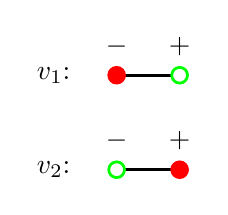
\begin{tikzpicture}  [scale=0.8]

\tikzstyle{every path}=[line width=1pt]

\newdimen\ms
\ms=0.1cm
\tikzstyle{s1}=[color=red,rectangle,inner sep=3.5]
\tikzstyle{c3}=[circle,inner sep={\ms/8},minimum size=4*\ms]
\tikzstyle{c2}=[circle,inner sep={\ms/8},minimum size=3*\ms]
\tikzstyle{c1}=[circle,inner sep={\ms/8},minimum size=2*\ms]
\tikzstyle{cs1}=[circle,inner sep={\ms/8},minimum size=1*\ms]

% Define positions of all observables


\coordinate (y113) at (-1.5,1.5);
\coordinate (y123) at (-2.5,1.5);

\coordinate (y114) at (-1.5,0);
\coordinate (y124) at (-2.5,0);

% draw contexts


\draw [color=black] (y113) -- (y123);

\draw [color=black] (y114) -- (y124);

% draw atoms

\draw (y114) coordinate[c1,fill=red, draw=red,label=above    :$+$];
\draw (y124) coordinate[c1,fill=white, draw=green,label=above:$-$];

\draw (y113) coordinate[c1,fill=white, draw=green,label=above:$+$];
\draw (y123) coordinate[c1,fill=red, draw=red,label=above    :$-$];

\draw (-3.5,1.5) node {$v_1$:};
\draw (-3.5,0) node {$v_2$:};

\end{tikzpicture}
}
}
&
$\qquad$
&
\begin{tabular}{|c|cc|}
\hline
$T$ &$-$& $+$\\
\hline
$v_1$&1&0\\
$v_2$&0&1\\
\hline
\end{tabular}
\end{tabular}
\end{center}
Probability distributions: subject to
$
\lambda_{-},
\lambda_{+} \ge 0$ and
\[
\lambda_{-} +
\lambda_{+}  = 1
\]
\begin{center}
\resizebox{.2\textwidth}{!}{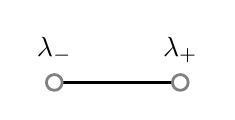
\begin{tikzpicture}  [scale=0.8]

\tikzstyle{every path}=[line width=1pt]

\newdimen\ms
\ms=0.1cm
\tikzstyle{s1}=[color=red,rectangle,inner sep=3.5]
\tikzstyle{c3}=[circle,inner sep={\ms/8},minimum size=4*\ms]
\tikzstyle{c2}=[circle,inner sep={\ms/8},minimum size=3*\ms]
\tikzstyle{c1}=[circle,inner sep={\ms/8},minimum size=2*\ms]
\tikzstyle{cs1}=[circle,inner sep={\ms/8},minimum size=1*\ms]

\coordinate (uuu) at (0,0);
\coordinate (uvu) at (2,0);


% draw contexts

\draw [color=black] (uuu) -- (uvu);

% draw atoms

\draw (uuu) coordinate[c1,fill=white, draw=Gray,label=above:$\lambda_{-}$];
\draw (uvu) coordinate[c1,fill=white, draw=Gray,label=above:$\lambda_{+}$];

\end{tikzpicture}
}
\end{center}

\end{frame}

%%%%%%%%%%%%%%%%%%%%%%%%%%%%%%%%%%%%%%%%%%%%%%%%%%%%%%%%%%%%%%%%%%%%%%%%%%%%%%%%%%%%%%%%%%%%%%%%%%%%%%%%%%%%%%%%%%

\section{Classical probabilities on multiple yet isolated/nonintertwining contexts}



%%%%%%%%%%%%%%%%%%%%%%%%%%%%%%%%%%%%%%%%%%%%%%%%%%%%%%%%%%%%%%%%%%%%%%%%%%%%%%%%%%%%%%%%%%%%%%%%%%%%%%%%%%%%%%%%%%

\begin{frame}
\begin{center}
{\large {\color{purple}$\;$}}
\end{center}

                                                    \vspace{1.15cm}

\centerline{\Large {\color{applegreen}{\color{blue}\decofourleft} \hspace{.15cm} {\it Multiple nonintertwining contexts} \hspace{.15cm} {\color{blue}\decofourright}}}

                                                    \vspace{1.15cm}
\begin{center}
{\large {\color{blue} $\;$}}
\end{center}

\end{frame}

%%%%%%%%%%%%%%%%%%%%%%%%%%%%%%%%%%%%%%%%%%%%%%%%%%%%%%%%%%%%%%%%%%%%%%%%%%%%%%%%%%%%%%%%%%%%%%%%%%%%%%%%%%%%%%%%%%

\begin{frame}[shrink=10]
 \frametitle{Classical probabilities on multiple yet isolated/nonintertwining contexts}

From this situation
on---by contemplating more than one of finitely many contexts/Boolean subalgebras/maximal observables/blocks---we
are dealing with \textbf{complementarity}.



\begin{itemize}

\item[(1)]  \textbf{Isolation principle---autonomous probabilities on isolated contexts}: In the case of isolated/nonintertwining---no common element(s)---contexts
every context is treated separately, as isolated entity.

Therefore, in particular,
probability distributions can be treated as isolated entities.

\pause

\item[(2)] \textbf{Multiplicativity of joint probabilities of events from different contexts}:
The joint probabilities and expectations are treated multiplicatively.

In particular,
for two contexts $\mathcal{C}_1$ and $\mathcal{C}_2$, in order to obtain all joint two-valued states $w$,
their respective two-valued states $u$ and $v$ can be multiplied:
\[
v_{ij} \big(a_s \wedge b_t\big) \equiv v_{ij}^{1,2} \big(a_s,b_t\big) = v^1_i (a_s) v^2_j (b_t),
\]
with
$a_s\in \mathcal{C}_1$,
$b_t\in \mathcal{C}_2$,
and $v^1_i$ and $v^2_j$ are two-valued states on those two contexts, respectively.

This can be understood either as consequence of the isolation principle, or in terms of the
product of two-valued states on multiple isolated contexts as follows.

\end{itemize}

\end{frame}

%%%%%%%%%%%%%%%%%%%%%%%%%%%%%%%%%%%%%%%%%%%%%%%%%%%%%%%%%%%%%%%%%%%%%%%%%%%%%%%%%%%%%%%%%%%%%%%%%%%%%%%%%%%%%%%%%%

\begin{frame}
 \frametitle{Classical probabilities on multiple yet isolated/nonintertwining contexts cntd.}

\begin{itemize}

\item[(1)]
\textbf{Truth assignments}:
per context
every experimental run only ``renders'' a \emph{single}  atomic outcome/event. All other  possible outcomes/events in these contexts
 ``do not occur''.

\pause
\item[(2)] \textbf{Encoding of truth assignments by two-valued state}:
\begin{itemize}

\item[(2.1)]
Define a binary two-valued state as a function $v$ on the elements of
the contexts/Boolean algebras such that $v(a_i)=1$ if the event/outcome $a_i$ occurs, otherwise the state $v$ vanishes.
Suppose an exhaustive search rendered $n$ such possible two-valued states $v_1,\ldots, v_n$.

\pause

\item[(2.2)] \textbf{Convexity}: A general classical probability distribution $P$ on the contexts $\mathcal{C}_1,\mathcal{C}_2,\ldots, \mathcal{C}_m$
can be written as a convex sum of two-valued states:
let $x \in  \bigcup\limits_{i=1}^{m}\mathcal{C}_i$
\[
\begin{split}
P(x) = \lambda_1 v_1(x) +\cdots + \lambda_n v_n(x),
\\
\text{with }
\lambda_1 +\cdots + \lambda_n=1
\text{ and }
\lambda_j \in \left[0,1\right]
, \;
j\in \left\{1,\ldots,n\right\}
.
\end{split}
\]

\end{itemize}
\end{itemize}

\end{frame}


%%%%%%%%%%%%%%%%%%%%%%%%%%%%%%%%%%%%%%%%%%%%%%%%%%%%%%%%%%%%%%%%%%%%%%%%%%%%%%%%%%%%%%%%%%%%%%%%%%%%%%%%%%%%%%%%%%

\begin{frame}
 \frametitle{Example: Two isolated/nonintertwining contexts ``containing'' two atoms each, two-valued states and probability distributions}

Two-valued states:

\begin{center}
\resizebox{.60\textwidth}{!}{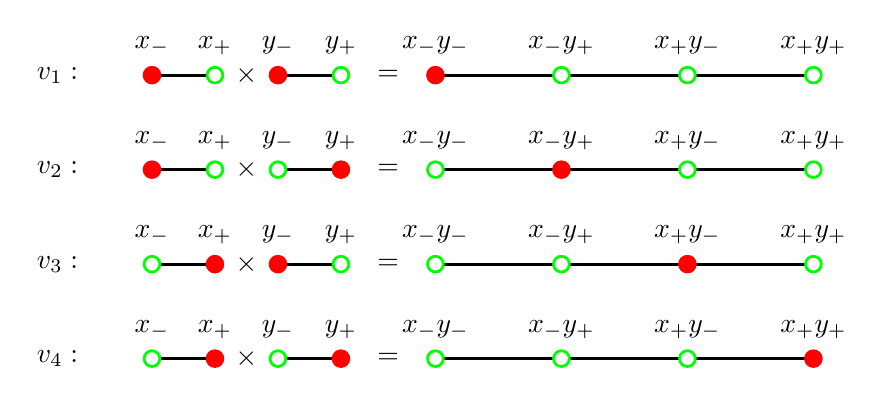
\begin{tikzpicture}  [scale=0.8]

\tikzstyle{every path}=[line width=1pt]

\newdimen\ms
\ms=0.1cm
\tikzstyle{s1}=[color=red,rectangle,inner sep=3.5]
\tikzstyle{c3}=[circle,inner sep={\ms/8},minimum size=4*\ms]
\tikzstyle{c2}=[circle,inner sep={\ms/8},minimum size=3*\ms]
\tikzstyle{c1}=[circle,inner sep={\ms/8},minimum size=2*\ms]
\tikzstyle{cs1}=[circle,inner sep={\ms/8},minimum size=1*\ms]

% Define positions of all observables



\coordinate (y111) at (-1.5,4.5);
\coordinate (y121) at (-2.5,4.5);
\coordinate (y211) at (-3.5,4.5);
\coordinate (y221) at (-4.5,4.5);

\coordinate (y112) at (-1.5,3);
\coordinate (y122) at (-2.5,3);
\coordinate (y212) at (-3.5,3);
\coordinate (y222) at (-4.5,3);

\coordinate (y113) at (-1.5,1.5);
\coordinate (y123) at (-2.5,1.5);
\coordinate (y213) at (-3.5,1.5);
\coordinate (y223) at (-4.5,1.5);

\coordinate (y114) at (-1.5,0);
\coordinate (y124) at (-2.5,0);
\coordinate (y214) at (-3.5,0);
\coordinate (y224) at (-4.5,0);

% draw contexts

\draw [color=black] (y111) -- (y121);
\draw [color=black] (y211) -- (y221);

\draw [color=black] (y112) -- (y122);
\draw [color=black] (y212) -- (y222);

\draw [color=black] (y113) -- (y123);
\draw [color=black] (y213) -- (y223);

\draw [color=black] (y114) -- (y124);
\draw [color=black] (y214) -- (y224);

% draw atoms

\draw (y114) coordinate[c1,fill=red, draw=red,label=above    :$y_+$];
\draw (y124) coordinate[c1,fill=white, draw=green,label=above:$y_-$];
\draw (y214) coordinate[c1,fill=red, draw=red,label=above    :$x_+$];
\draw (y224) coordinate[c1,fill=white, draw=green,label=above:$x_-$];

\draw (y113) coordinate[c1,fill=white, draw=green,label=above:$y_+$];
\draw (y123) coordinate[c1,fill=red, draw=red,label=above    :$y_-$];
\draw (y213) coordinate[c1,fill=red, draw=red,label=above    :$x_+$];
\draw (y223) coordinate[c1,fill=white, draw=green,label=above:$x_-$];

\draw (y112) coordinate[c1,fill=red, draw=red,label=above    :$y_+$];
\draw (y122) coordinate[c1,fill=white, draw=green,label=above:$y_-$];
\draw (y212) coordinate[c1,fill=white, draw=green,label=above:$x_+$];
\draw (y222) coordinate[c1,fill=red, draw=red,label=above    :$x_-$];

\draw (y111) coordinate[c1,fill=white, draw=green,label=above:$y_+$];
\draw (y121) coordinate[c1,fill=red, draw=red,label=above    :$y_-$];
\draw (y211) coordinate[c1,fill=white, draw=green,label=above:$x_+$];
\draw (y221) coordinate[c1,fill=red, draw=red,label=above    :$x_-$];

\draw (-3,4.5) node {$\times$};
\draw (-3,3) node {$\times$};
\draw (-3,1.5) node {$\times$};
\draw (-3,0) node {$\times$};

\draw (-0.75,4.5) node {$=$};
\draw (-0.75,3) node {$=$};
\draw (-0.75,1.5) node {$=$};
\draw (-0.75,0) node {$=$};

\draw (-6,4.5) node {$v_1:$};
\draw (-6,3) node {$v_2:$};
\draw (-6,1.5) node {$v_3:$};
\draw (-6,0) node {$v_4:$};

% Define positions of all observables

\coordinate (ccu) at (0,4.5);
\coordinate (cdu) at (2,4.5);
\coordinate (dcu) at (4,4.5);
\coordinate (ddu) at (6,4.5);

\coordinate (cuc) at (0,3);
\coordinate (cud) at (2,3);
\coordinate (duc) at (4,3);
\coordinate (dud) at (6,3);

\coordinate (ucc) at (0,1.5);
\coordinate (ucd) at (2,1.5);
\coordinate (udc) at (4,1.5);
\coordinate (udd) at (6,1.5);

\coordinate (uuu) at (0,0);
\coordinate (uvu) at (2,0);
\coordinate (vuu) at (4,0);
\coordinate (vvu) at (6,0);

% draw contexts

\draw [color=black] (ccu) -- (ddu);
\draw [color=black] (cuc) -- (dud);
\draw [color=black] (ucc) -- (udd);
\draw [color=black] (uuu) -- (vvu);



% draw atoms

\draw (ccu) coordinate[c1,fill=red, draw=red,label=above:$x_-  y_-$];
\draw (cdu) coordinate[c1,fill=white, draw=green,label=above:$x_-  y_+$];
\draw (dcu) coordinate[c1,fill=white, draw=green,label=above:$x_+  y_-$];
\draw (ddu) coordinate[c1,fill=white, draw=green,label=above:$x_+  y_+$];

\draw (cuc) coordinate[c1,fill=white, draw=green,label=above:$x_-  y_-$];
\draw (cud) coordinate[c1,fill=red, draw=red,label=above:$x_-  y_+$];
\draw (duc) coordinate[c1,fill=white, draw=green,label=above:$x_+  y_-$];
\draw (dud) coordinate[c1,fill=white, draw=green,label=above:$x_+  y_+$];

\draw (ucc) coordinate[c1,fill=white, draw=green,label=above:$x_-  y_-$];
\draw (ucd) coordinate[c1,fill=white, draw=green,label=above:$x_-  y_+$];
\draw (udc) coordinate[c1,fill=red, draw=red,label=above:$x_+  y_-$];
\draw (udd) coordinate[c1,fill=white, draw=green,label=above:$x_+  y_+$];

\draw (uuu) coordinate[c1,fill=white, draw=green,label=above:$x_-  y_-$];
\draw (uvu) coordinate[c1,fill=white, draw=green,label=above:$x_-  y_+$];
\draw (vuu) coordinate[c1,fill=white, draw=green,label=above:$x_+  y_-$];
\draw (vvu) coordinate[c1,fill=red, draw=red,label=above:    $x_+  y_+$];



\end{tikzpicture}
}
\end{center}
Probability distributions:
$
\lambda_{x_-  y_-},
\lambda_{x_-  y_+},
\lambda_{x_+  y_-},
\lambda_{x_+  y_+} \ge 0$ and
\[
\lambda_{x_-  y_-} +
\lambda_{x_-  y_+} +
\lambda_{x_+  y_-} +
\lambda_{x_+  y_+}  = 1
\]
\begin{center}
\begin{tabular}{ccc}
\resizebox{.35\textwidth}{!}{
\begin{tabular}{|c|cccc|}
\hline
$T$ &$x_-  y_-$& $x_-  y_+$& $x_+  y_-$& $x_+  y_+$\\
\hline
$v_1$&1&0&0&0\\
$v_2$&0&1&0&0\\
$v_3$&0&0&1&0\\
$v_4$&0&0&0&1\\
\hline
\end{tabular}
}
&
$\qquad$
&
\raisebox{0cm}{
\resizebox{.3\textwidth}{!}{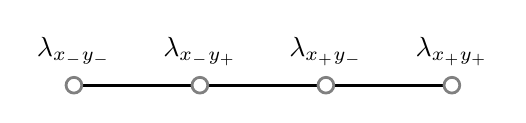
\begin{tikzpicture}  [scale=0.8]

\tikzstyle{every path}=[line width=1pt]

\newdimen\ms
\ms=0.1cm
\tikzstyle{s1}=[color=red,rectangle,inner sep=3.5]
\tikzstyle{c3}=[circle,inner sep={\ms/8},minimum size=4*\ms]
\tikzstyle{c2}=[circle,inner sep={\ms/8},minimum size=3*\ms]
\tikzstyle{c1}=[circle,inner sep={\ms/8},minimum size=2*\ms]
\tikzstyle{cs1}=[circle,inner sep={\ms/8},minimum size=1*\ms]

\coordinate (uuu) at (0,0);
\coordinate (uvu) at (2,0);
\coordinate (vuu) at (4,0);
\coordinate (vvu) at (6,0);

% draw contexts

\draw [color=black] (uuu) -- (vvu);

% draw atoms

\draw (uuu) coordinate[c1,fill=white, draw=Gray,label=above:$\lambda_{x_-  y_-}$];
\draw (uvu) coordinate[c1,fill=white, draw=Gray,label=above:$\lambda_{x_-  y_+}$];
\draw (vuu) coordinate[c1,fill=white, draw=Gray,label=above:$\lambda_{x_+  y_-}$];
\draw (vvu) coordinate[c1,fill=white, draw=Gray,label=above:$\lambda_{x_+  y_+}$];

\end{tikzpicture}
}
}
\end{tabular}
\end{center}

\end{frame}

%%%%%%%%%%%%%%%%%%%%%%%%%%%%%%%%%%%%%%%%%%%%%%%%%%%%%%%%%%%%%%%%%%%%%%%%%%%%%%%%%%%%%%%%%%%%%%%%%%%%%%%%%%%%%%%%%%


\section{Classical probabilities on multiple intertwining Boolean contexts}

%%%%%%%%%%%%%%%%%%%%%%%%%%%%%%%%%%%%%%%%%%%%%%%%%%%%%%%%%%%%%%%%%%%%%%%%%%%%%%%%%%%%%%%%%%%%%%%%%%%%%%%%%%%%%%%%%%

\begin{frame}
\begin{center}
{\large {\color{purple}$\;$}}
\end{center}

                                                    \vspace{1.15cm}

\centerline{\Large {\color{applegreen}{\color{blue}\decofourleft} \hspace{.15cm} {\it Multiple intertwining contexts} \hspace{.15cm} {\color{blue}\decofourright}}}

                                                    \vspace{1.15cm}
\begin{center}
{\large {\color{blue} $\;$}}
\end{center}

\end{frame}

%%%%%%%%%%%%%%%%%%%%%%%%%%%%%%%%%%%%%%%%%%%%%%%%%%%%%%%%%%%%%%%%%%%%%%%%%%%%%%%%%%%%%%%%%%%%%%%%%%%%%%%%%%%%%%%%%%

\begin{frame}%[shrink=10]
 \frametitle{Classical probabilities on multiple intertwining Boolean contexts}

In these configurations we are still assuming that all pairs of atomic, elementary propositions formalized by unit
vectors/orthogonal projection operators/one-dimensional subspaces are mutually \emph{separable} by some two-valued measure; cf.
the Kochen-Specker demarcation criterion Theorem 0,
DOI \href{https://doi.org/10.1512/iumj.1957.6.56050}{10.1512/iumj.1957.6.56050}.


\begin{itemize}

\item[(1)] \textbf{Computing extreme states satisfying exclusivity}: Compute all two-valued states on the propositional structure.

\pause

\item[(2)] \textbf{Convex combination}: the probability distributions on a particular atomic, elementary proposition are convex combinations
of the respective nonzero two-valued states on them. The convex sum of all the weights is normalized to 1.



\end{itemize}

\end{frame}


%%%%%%%%%%%%%%%%%%%%%%%%%%%%%%%%%%%%%%%%%%%%%%%%%%%%%%%%%%%%%%%%%%%%%%%%%%%%%%%%%%%%%%%%%%%%%%%%%%%%%%%%%%%%%%%%%%

\begin{frame}
 \frametitle{Classical probabilities on multiple intertwining Boolean contexts cntd.}

\begin{itemize}

\item[(1)]
\textbf{Truth assignments}:
per context
every experimental run only ``renders'' a \emph{single}  atomic outcome/event. All other  possible outcomes/events in these contexts
 ``do not occur''.

\pause
\item[(2)] \textbf{Encoding of truth assignments by two-valued state}:
\begin{itemize}

\item[(2.1)]
Define a binary two-valued state as a function $v$ on the elements of
the contexts/Boolean algebras such that $v(a_i)=1$ if the event/outcome $a_i$ occurs, otherwise the state $v$ vanishes.
Suppose an exhaustive search rendered $n$ such possible two-valued states $v_1,\ldots, v_n$.


\pause

\item[(2.2)] \textbf{Convexity}: A general classical probability distribution $P$ on the contexts $\mathcal{C}_1,\mathcal{C}_2,\ldots, \mathcal{C}_m$
can be written as a convex sum of two-valued states:
let $x \in  \bigcup\limits_{i=1}^{m}\mathcal{C}_i$
\[
\begin{split}
P(x) = \lambda_1 v_1(x) +\cdots + \lambda_n v_n(x),
\\
\text{with }
\lambda_1 +\cdots + \lambda_n=1
\text{ and }
\lambda_j \in \left[0,1\right]
, \;
j\in \left\{1,\ldots,n\right\}
.
\end{split}
\]

\end{itemize}
\end{itemize}

\end{frame}


%%%%%%%%%%%%%%%%%%%%%%%%%%%%%%%%%%%%%%%%%%%%%%%%%%%%%%%%%%%%%%%%%%%%%%%%%%%%%%%%%%%%%%%%%%%%%%%%%%%%%%%%%%%%%%%%%%

\begin{frame}[shrink=4] %
 \frametitle{Detour: a revisionist history of classical probabilities on intertwining contexts}

\begin{itemize}

\item[Q]
Cabello, in a
\href{https://www.youtube.com/watch?v=5r6J-PQVo_s&t=1827s}{historic review @ 30m27s of https://youtu.be/5r6J-PQVo\_s},
states that:
\emph{``$\ldots$~it's a pity that Pitowsky who had all  the background needed to go further, stopped by just noticing
that Bell inequalities are a subset of the Boole inequalities.''}

\pause

\item[R]
My response to that:

\begin{itemize}

\item[R1]
Pitowsky turned his attention to the (arguably) much stronger result of Kochen {\&} Specker, and
\href{https://doi.org/10.1063/1.532334}{indeterminacy}.

\pause

\item[R2]
Why should one do this from a pragmatic point of view?
Arguments involving interwining contexts needed to study qutrit or qudit  systems with Hilbert spaces of
dimension three and higher (no intertwined observables in $d=2$)
that are difficult to operationalize even to this day.

\pause

\item[R3]
Indeed, on what grounds is it better to certify differences between quantum and classical predictions
from counterfactual constructions of complementary intertwined rather than isolated contexts?
Why is it not even sufficient for this purpose to consider the quantitative difference of a single quantum versus a classical expectation value?
Why involve three (Suppes Zanotti) or four (CHSH) such expectation values?

\end{itemize}
\end{itemize}

\end{frame}


%%%%%%%%%%%%%%%%%%%%%%%%%%%%%%%%%%%%%%%%%%%%%%%%%%%%%%%%%%%%%%%%%%%%%%%%%%%%%%%%%%%%%%%%%%%%%%%%%%%%%%%%%%%%%%%%%%


\begin{frame}[shrink=10]
 \frametitle{Detour to a revisionist history of classical probabilities on intertwining contexts cntd.}

Trigger warning of self-promotion:
nevertheless---because I fiddled around with partition logics---my 2001 arXiv paper
\href{https://arxiv.org/abs/quant-ph/0012066}{``On generalized probabilities:
correlation polytopes for automaton logic and generalized urn models~$\ldots$'' @  arXiv:quant-ph/0012066}
considers the hull problem for the ``Specker bug'' (a true-implies-false gadget, see later discussion)
and similar intertwining propositional structures already in its ``modern form'' via the Travis matrix.

The paper was written for the Fifth Biannual IQSA Conference "Quantum Structures' 2000"  in Cesena, Italy, March 31 -- April 5, 2001,
but for personal reasons I never made it to Cesena. I even submitted it (to Greechie) for the proceedings  but never heard of it afterwards.

I started contemplating generalized hull problems for intertwining contexts with the 2nd version of the
paper stating that \emph{``The (nonclassical) correlation polytope corresponding to $L$ can be defined as the
convex hull of all two-valued states thereon.''}
Version 3 contains a hull computation by using a Viennese package bei Kreuzer and Skarke.

But, unlike the famous 2008
\href{https://doi.org//10.1103/PhysRevLett.101.020403}
{Klyachko, Can, Binicio\ifmmode \breve{g}\else \u{g}\fi{}lu and Shumovsky paper DOI: 10.1103/PhysRevLett.101.020403}
I did not consider actual violations of the hull inequalities by quantum predictions.


\end{frame}


%%%%%%%%%%%%%%%%%%%%%%%%%%%%%%%%%%%%%%%%%%%%%%%%%%%%%%%%%%%%%%%%%%%%%%%%%%%%%%%%%%%%%%%%%%%%%%%%%%%%%%%%%%%%%%%%%%


\begin{frame}
 \frametitle{Classical probabilities on two intertwining Boolean contexts with three atoms each (``two different tripods with one common leg'')}

Two-valued states (two representations by hypergraphs, one meaning):

\begin{center}
\resizebox{.90\textwidth}{!}{
\begin{tabular}{ c c c c c }
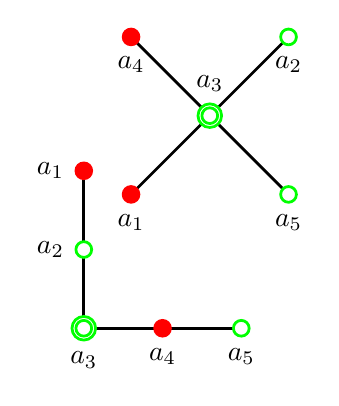
\begin{tikzpicture}  [scale=1]

\tikzstyle{every path}=[line width=1pt]

\newdimen\ms
\ms=0.1cm
\tikzstyle{s1}=[color=red,rectangle,inner sep=3.5]
\tikzstyle{c3}=[circle,inner sep={\ms/8},minimum size=5*\ms]
\tikzstyle{c2}=[circle,inner sep={\ms/8},minimum size=3*\ms]
\tikzstyle{c1}=[circle,inner sep={\ms/8},minimum size=2*\ms]

% Define positions of all observables

\coordinate (a21) at ({0.6+0},{1.7+0});
\coordinate (a22) at ({0.6+2},{1.7+2});
\coordinate (a23) at ({0.6+1},{1.7+1});
\coordinate (a24) at ({0.6+0},{1.7+2});
\coordinate (a25) at ({0.6+2},{1.7+0});

% draw contexts

\draw [color=black] (a21) -- (a22);
\draw [color=black] (a24) -- (a25);

% draw atoms

\draw (a21) coordinate[c1,draw=red,fill=red,label=below:$a_1$];

\draw (a22) coordinate[c1,draw=green,fill=white,label=below:$a_2$];

\draw (a23) coordinate[c2,draw=green,fill=white,label=above:$a_3$];
\draw (a23) coordinate[c1,draw=green,fill=white];

\draw (a24) coordinate[c1,draw=red,fill=red,label=below:$a_4$];

\draw (a25) coordinate[c1,draw=green,fill=white,label=below:$a_5$];

%%%%%%%%%%%%%%%%%%%%%%%%%%%%%%%%%%%%%%%%%%%%%%%%%%%%%%%%%%%%%%%%%%%%

% Define positions of all observables

\coordinate (a1) at (0,2);
\coordinate (a2) at (0,1);
\coordinate (a3) at (0,0);
\coordinate (a4) at (1,0);
\coordinate (a5) at (2,0);

% draw contexts

\draw [color=black] (a1) -- (a3);
\draw [color=black] (a3) -- (a5);

% draw atoms

\draw (a1) coordinate[c1,draw=red,fill=red,label=left:$a_1$];

\draw (a2) coordinate[c1,draw=green,fill=white,label=left:$a_2$];

\draw (a3) coordinate[c2,draw=green,fill=white,label=below:$a_3$];
\draw (a3) coordinate[c1,draw=green,fill=white];

\draw (a4) coordinate[c1,draw=red,fill=red,label=below:$a_4$];

\draw (a5) coordinate[c1,draw=green,fill=white,label=below:$a_5$];


\end{tikzpicture}
&
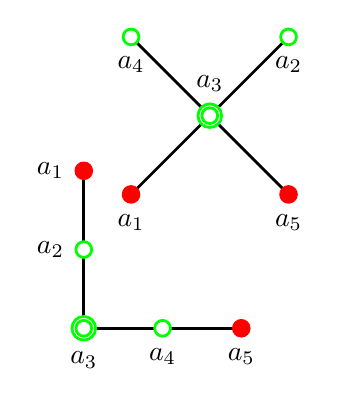
\begin{tikzpicture}  [scale=1]

\tikzstyle{every path}=[line width=1pt]

\newdimen\ms
\ms=0.1cm
\tikzstyle{s1}=[color=red,rectangle,inner sep=3.5]
\tikzstyle{c3}=[circle,inner sep={\ms/8},minimum size=5*\ms]
\tikzstyle{c2}=[circle,inner sep={\ms/8},minimum size=3*\ms]
\tikzstyle{c1}=[circle,inner sep={\ms/8},minimum size=2*\ms]

% Define positions of all observables

\coordinate (a21) at ({0.6+0},{1.7+0});
\coordinate (a22) at ({0.6+2},{1.7+2});
\coordinate (a23) at ({0.6+1},{1.7+1});
\coordinate (a24) at ({0.6+0},{1.7+2});
\coordinate (a25) at ({0.6+2},{1.7+0});

% draw contexts

\draw [color=black] (a21) -- (a22);
\draw [color=black] (a24) -- (a25);

% draw atoms

\draw (a21) coordinate[c1,draw=red,fill=red,label=below:$a_1$];

\draw (a22) coordinate[c1,draw=green,fill=white,label=below:$a_2$];

\draw (a23) coordinate[c2,draw=green,fill=white,label=above:$a_3$];
\draw (a23) coordinate[c1,draw=green,fill=white];

\draw (a24) coordinate[c1,draw=green,fill=white,label=below:$a_4$];

\draw (a25) coordinate[c1,draw=red,fill=red,label=below:$a_5$];

%%%%%%%%%%%%%%%%%%%%%%%%%%%%%%%%%%%%%%%%%%%%%%%%%%%%%%%%%%%%%%%%%%%%

% Define positions of all observables

\coordinate (a1) at (0,2);
\coordinate (a2) at (0,1);
\coordinate (a3) at (0,0);
\coordinate (a4) at (1,0);
\coordinate (a5) at (2,0);

% draw contexts

\draw [color=black] (a1) -- (a3);
\draw [color=black] (a3) -- (a5);

% draw atoms

\draw (a1) coordinate[c1,draw=red,fill=red,label=left:$a_1$];

\draw (a2) coordinate[c1,draw=green,fill=white,label=left:$a_2$];

\draw (a3) coordinate[c2,draw=green,fill=white,label=below:$a_3$];
\draw (a3) coordinate[c1,draw=green,fill=white];

\draw (a4) coordinate[c1,draw=green,fill=white,label=below:$a_4$];

\draw (a5) coordinate[c1,draw=red,fill=red,label=below:$a_5$];


\end{tikzpicture}
&
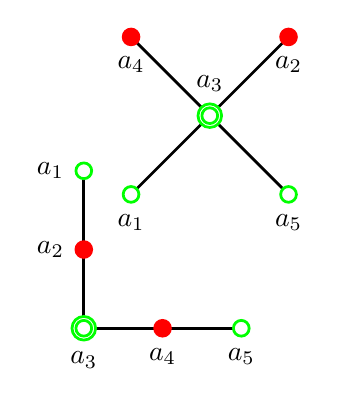
\begin{tikzpicture}  [scale=1]

\tikzstyle{every path}=[line width=1pt]

\newdimen\ms
\ms=0.1cm
\tikzstyle{s1}=[color=red,rectangle,inner sep=3.5]
\tikzstyle{c3}=[circle,inner sep={\ms/8},minimum size=5*\ms]
\tikzstyle{c2}=[circle,inner sep={\ms/8},minimum size=3*\ms]
\tikzstyle{c1}=[circle,inner sep={\ms/8},minimum size=2*\ms]

% Define positions of all observables

\coordinate (a21) at ({0.6+0},{1.7+0});
\coordinate (a22) at ({0.6+2},{1.7+2});
\coordinate (a23) at ({0.6+1},{1.7+1});
\coordinate (a24) at ({0.6+0},{1.7+2});
\coordinate (a25) at ({0.6+2},{1.7+0});

% draw contexts

\draw [color=black] (a21) -- (a22);
\draw [color=black] (a24) -- (a25);

% draw atoms

\draw (a21) coordinate[c1,draw=green,fill=white,label=below:$a_1$];

\draw (a22) coordinate[c1,draw=red,fill=red,label=below:$a_2$];

\draw (a23) coordinate[c2,draw=green,fill=white,label=above:$a_3$];
\draw (a23) coordinate[c1,draw=green,fill=white];

\draw (a24) coordinate[c1,draw=red,fill=red,label=below:$a_4$];

\draw (a25) coordinate[c1,draw=green,fill=white,label=below:$a_5$];

%%%%%%%%%%%%%%%%%%%%%%%%%%%%%%%%%%%%%%%%%%%%%%%%%%%%%%%%%%%%%%%%%%%%

% Define positions of all observables

\coordinate (a1) at (0,2);
\coordinate (a2) at (0,1);
\coordinate (a3) at (0,0);
\coordinate (a4) at (1,0);
\coordinate (a5) at (2,0);

% draw contexts

\draw [color=black] (a1) -- (a3);
\draw [color=black] (a3) -- (a5);

% draw atoms

\draw (a1) coordinate[c1,draw=green,fill=white,label=left:$a_1$];

\draw (a2) coordinate[c1,draw=red,fill=red,label=left:$a_2$];

\draw (a3) coordinate[c2,draw=green,fill=white,label=below:$a_3$];
\draw (a3) coordinate[c1,draw=green,fill=white];

\draw (a4) coordinate[c1,draw=red,fill=red,label=below:$a_4$];

\draw (a5) coordinate[c1,draw=green,fill=white,label=below:$a_5$];


\end{tikzpicture}
&
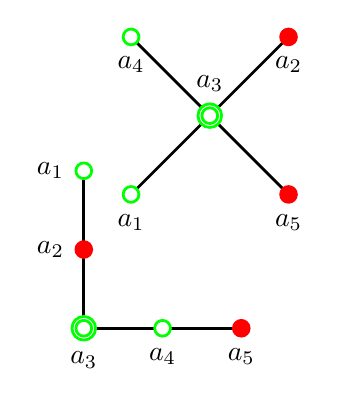
\begin{tikzpicture}  [scale=1]

\tikzstyle{every path}=[line width=1pt]

\newdimen\ms
\ms=0.1cm
\tikzstyle{s1}=[color=red,rectangle,inner sep=3.5]
\tikzstyle{c3}=[circle,inner sep={\ms/8},minimum size=5*\ms]
\tikzstyle{c2}=[circle,inner sep={\ms/8},minimum size=3*\ms]
\tikzstyle{c1}=[circle,inner sep={\ms/8},minimum size=2*\ms]

% Define positions of all observables

\coordinate (a21) at ({0.6+0},{1.7+0});
\coordinate (a22) at ({0.6+2},{1.7+2});
\coordinate (a23) at ({0.6+1},{1.7+1});
\coordinate (a24) at ({0.6+0},{1.7+2});
\coordinate (a25) at ({0.6+2},{1.7+0});

% draw contexts

\draw [color=black] (a21) -- (a22);
\draw [color=black] (a24) -- (a25);

% draw atoms

\draw (a21) coordinate[c1,draw=green,fill=white,label=below:$a_1$];

\draw (a22) coordinate[c1,draw=red,fill=red,label=below:$a_2$];

\draw (a23) coordinate[c2,draw=green,fill=white,label=above:$a_3$];
\draw (a23) coordinate[c1,draw=green,fill=white];

\draw (a24) coordinate[c1,draw=green,fill=white,label=below:$a_4$];

\draw (a25) coordinate[c1,draw=red,fill=red,label=below:$a_5$];

%%%%%%%%%%%%%%%%%%%%%%%%%%%%%%%%%%%%%%%%%%%%%%%%%%%%%%%%%%%%%%%%%%%%

% Define positions of all observables

\coordinate (a1) at (0,2);
\coordinate (a2) at (0,1);
\coordinate (a3) at (0,0);
\coordinate (a4) at (1,0);
\coordinate (a5) at (2,0);

% draw contexts

\draw [color=black] (a1) -- (a3);
\draw [color=black] (a3) -- (a5);

% draw atoms

\draw (a1) coordinate[c1,draw=green,fill=white,label=left:$a_1$];

\draw (a2) coordinate[c1,draw=red,fill=red,label=left:$a_2$];

\draw (a3) coordinate[c2,draw=green,fill=white,label=below:$a_3$];
\draw (a3) coordinate[c1,draw=green,fill=white];

\draw (a4) coordinate[c1,draw=green,fill=white,label=below:$a_4$];

\draw (a5) coordinate[c1,draw=red,fill=red,label=below:$a_5$];


\end{tikzpicture}
&
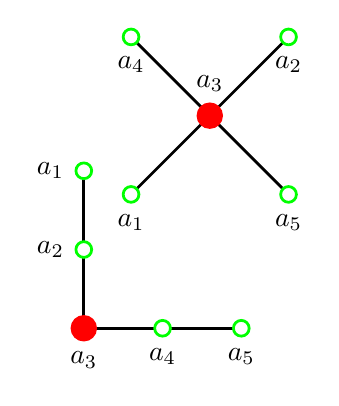
\begin{tikzpicture}  [scale=1]

\tikzstyle{every path}=[line width=1pt]

\newdimen\ms
\ms=0.1cm
\tikzstyle{s1}=[color=red,rectangle,inner sep=3.5]
\tikzstyle{c3}=[circle,inner sep={\ms/8},minimum size=5*\ms]
\tikzstyle{c2}=[circle,inner sep={\ms/8},minimum size=3*\ms]
\tikzstyle{c1}=[circle,inner sep={\ms/8},minimum size=2*\ms]

% Define positions of all observables

\coordinate (a21) at ({0.6+0},{1.7+0});
\coordinate (a22) at ({0.6+2},{1.7+2});
\coordinate (a23) at ({0.6+1},{1.7+1});
\coordinate (a24) at ({0.6+0},{1.7+2});
\coordinate (a25) at ({0.6+2},{1.7+0});

% draw contexts

\draw [color=black] (a21) -- (a22);
\draw [color=black] (a24) -- (a25);

% draw atoms

\draw (a21) coordinate[c1,draw=green,fill=white,label=below:$a_1$];

\draw (a22) coordinate[c1,draw=green,fill=white,label=below:$a_2$];

\draw (a23) coordinate[c2,draw=red,fill=red,label=above:$a_3$];
\draw (a23) coordinate[c1,draw=red,fill=red];

\draw (a24) coordinate[c1,draw=green,fill=white,label=below:$a_4$];

\draw (a25) coordinate[c1,draw=green,fill=white,label=below:$a_5$];

%%%%%%%%%%%%%%%%%%%%%%%%%%%%%%%%%%%%%%%%%%%%%%%%%%%%%%%%%%%%%%%%%%%%

% Define positions of all observables

\coordinate (a1) at (0,2);
\coordinate (a2) at (0,1);
\coordinate (a3) at (0,0);
\coordinate (a4) at (1,0);
\coordinate (a5) at (2,0);

% draw contexts

\draw [color=black] (a1) -- (a3);
\draw [color=black] (a3) -- (a5);

% draw atoms

\draw (a1) coordinate[c1,draw=green,fill=white,label=left:$a_1$];

\draw (a2) coordinate[c1,draw=green,fill=white,label=left:$a_2$];

\draw (a3) coordinate[c2,draw=red,fill=red,label=below:$a_3$];
\draw (a3) coordinate[c1,draw=red,fill=red];

\draw (a4) coordinate[c1,draw=green,fill=white,label=below:$a_4$];

\draw (a5) coordinate[c1,draw=green,fill=white,label=below:$a_5$];


\end{tikzpicture}
\\
$v_1$&
$v_2$&
$v_3$&
$v_4$&
$v_5$\\
\end{tabular}
}
\end{center}

Probability distributions:
$\lambda_{i}\ge 0$ for $i\in \{1,\ldots ,5\}$ and $ \sum_{i=1}^5 \lambda_{i} = 1 $.
\begin{center}
\begin{tabular}{ccc}
\resizebox{.35\textwidth}{!}{
\begin{tabular}{|c|ccccc|}
\hline
$T$ &$a_1$& $a_2$& $a_3$& $a_4$& $a_5$\\
\hline
$v_1$&1&0&0&1&0\\
$v_2$&1&0&0&0&1\\
$v_3$&0&1&0&1&0\\
$v_4$&0&1&0&0&1\\
$v_5$&0&0&1&0&0\\
\hline
\end{tabular}
}
&
$\qquad$
&
\raisebox{-1cm}{
\resizebox{.35\textwidth}{!}{
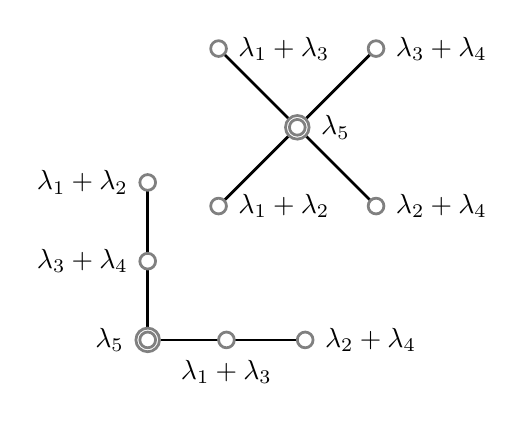
\begin{tikzpicture}  [scale=1]

\tikzstyle{every path}=[line width=1pt]

\newdimen\ms
\ms=0.1cm
\tikzstyle{s1}=[color=red,rectangle,inner sep=3.5]
\tikzstyle{c3}=[circle,inner sep={\ms/8},minimum size=5*\ms]
\tikzstyle{c2}=[circle,inner sep={\ms/8},minimum size=3*\ms]
\tikzstyle{c1}=[circle,inner sep={\ms/8},minimum size=2*\ms]

% Define positions of all observables

\coordinate (a21) at ({0.9+0},{1.7+0});
\coordinate (a22) at ({0.9+2},{1.7+2});
\coordinate (a23) at ({0.9+1},{1.7+1});
\coordinate (a24) at ({0.9+0},{1.7+2});
\coordinate (a25) at ({0.9+2},{1.7+0});

% draw contexts

\draw [color=black] (a21) -- (a22);
\draw [color=black] (a24) -- (a25);

% draw atoms

\draw (a21) coordinate[c1,draw=Gray,fill=white,label=right:$\lambda_1+\lambda_2$];

\draw (a22) coordinate[c1,draw=Gray,fill=white,label=right:$\lambda_3+\lambda_4$];

\draw (a23) coordinate[c2,draw=Gray,fill=white,label=right:$\lambda_5$];
\draw (a23) coordinate[c1,draw=Gray,fill=white];

\draw (a24) coordinate[c1,draw=Gray,fill=white,label=right:$\lambda_1+\lambda_3$];

\draw (a25) coordinate[c1,draw=Gray,fill=white,label=right:$\lambda_2+\lambda_4$];

%%%%%%%%%%%%%%%%%%%%%%%%%%%%%%%%%%%%%%%%%%%%%%%%%%%%%%%%%%%%%%%%%%%%

% Define positions of all observables

\coordinate (a1) at (0,2);
\coordinate (a2) at (0,1);
\coordinate (a3) at (0,0);
\coordinate (a4) at (1,0);
\coordinate (a5) at (2,0);

% draw contexts

\draw [color=black] (a1) -- (a3);
\draw [color=black] (a3) -- (a5);

% draw atoms

\draw (a1) coordinate[c1,draw=Gray,fill=white,label=left:$\lambda_1+\lambda_2$];

\draw (a2) coordinate[c1,draw=Gray,fill=white,label=left:$\lambda_3+\lambda_4$];

\draw (a3) coordinate[c2,draw=Gray,fill=white,label=left:$\lambda_5$];
\draw (a3) coordinate[c1,draw=Gray,fill=white];

\draw (a4) coordinate[c1,draw=Gray,fill=white,label=below:$\lambda_1+\lambda_3$];

\draw (a5) coordinate[c1,draw=Gray,fill=white,label=right:$\lambda_2+\lambda_4$];


\end{tikzpicture}
}
}
\end{tabular}
\end{center}

\end{frame}

%%%%%%%%%%%%%%%%%%%%%%%%%%%%%%%%%%%%%%%%%%%%%%%%%%%%%%%%%%%%%%%%%%%%%%%%%%%%%%%%%%%%%%%%%%%%%%%%%%%%%%%%%%%%%%%%%%

\section{Boole's ``Conditions of Possible Experience''}

%%%%%%%%%%%%%%%%%%%%%%%%%%%%%%%%%%%%%%%%%%%%%%%%%%%%%%%%%%%%%%%%%%%%%%%%%%%%%%%%%%%%%%%%%%%%%%%%%%%%%%%%%%%%%%%%%%

\begin{frame}
\begin{center}
{\large {\color{purple}$\;$}}
\end{center}

                                                    \vspace{1.15cm}

\centerline{\Large {\color{applegreen}{\color{blue}\decofourleft} \hspace{.15cm} {\it Boole's ``Conditions of Possible Experience''} \hspace{.15cm} {\color{blue}\decofourright}}}

                                                    \vspace{1.15cm}
\begin{center}
{\large {\color{blue} $\;$}}
\end{center}

\end{frame}

%%%%%%%%%%%%%%%%%%%%%%%%%%%%%%%%%%%%%%%%%%%%%%%%%%%%%%%%%%%%%%%%%%%%%%%%%%%%%%%%%%%%%%%%%%%%%%%%%%%%%%%%%%%%%%%%%%

\begin{frame}
 \frametitle{Boole's ``Conditions of Possible Experience''}

Geometric (re)interpretation/representation of probability distributions as convex polytope by
Froissart DOI \href{https://doi.org/10.1007/BF02903286}{10.1007/BF02903286},
Garg {\&} Mermin DOI \href{https://doi.org/10.1007/BF00741645}{10.1007/BF00741645},
Pitowsky DOI \href{https://doi.org/10.1063/1.527066}{10.1063/1.527066}, \href{https://doi.org/10.1007/BFb0021186}{10.1007/BFb0021186},
Tsirelson and others.

\begin{itemize}

\item[1.]
Form a ``bouquet'' of $n$ ``relevant'' (that is up to you what you include/exclude) combinations of (joint) dichotomic elementary outcomes/events.
Arrange these as $n$-tuples and consider them as ``row vectors'' wrt some orthonormal basis.

\pause

\item[2.]
Suppose there are $k$ two-valued states on the pertinent contexts.
Apply these valuations to the chosen $n$ combinations of (joint) dichotomic elementary outcomes/events, and
form $k$ row vectors from the resulting $n$-tuples.

\pause

\item[3.]
Interprete the $n$-tuples as vectors in an $n$-dimensional (real or complex) Hilbert space.

``Stack' these row vectors formed in 2. on top of each other.
The resulting matrix is a (kind of) Travis matrix.



\end{itemize}
\end{frame}

%%%%%%%%%%%%%%%%%%%%%%%%%%%%%%%%%%%%%%%%%%%%%%%%%%%%%%%%%%%%%%%%%%%%%%%%%%%%%%%%%%%%%%%%%%%%%%%%%%%%%%%%%%%%%%%%%%


\begin{frame}
 \frametitle{Boole's ``Conditions of Possible Experience'' cntd.}


\begin{itemize}

\item[4.]

Consider the convex polytope formed by interpreting the $k$ $n$-tuples as \emph{vertices} of the polytope.

\pause

\item[5.]
According to the Farkas-Minkowski-Weyl ``main'' representation theorem
(DOI
\href{https://doi.org/10.1007/978-1-4613-8431-1}{10.1007/978-1-4613-8431-1})
this convex polytope (aka convex cone or just cone)
has an equivalent representation as
\begin{itemize}
\item[5.1.]
its \emph{vertices} (aka the cone is finitely generated; cf. Alexander Schrijver, ``Theory of Linear and Integer Programming'', Wiley, 1986); as well as
\item[5.2.]
its \emph{facets} or intersecting half-spaces  (aka the cone is polyhedral)
obtained by the \emph{hull computation}.
\end{itemize}

\pause

\item[6.]
These facet (in)equalities represent Boole-Bell type ``conditions of possible (classical) experience''.


\end{itemize}

If one is dealing with expectation values then instead of the two-valued states the (affine) transformed expectation values have to be inserted for the Travis matrix.

\end{frame}





\section{Programs to compute optimal Boole-Bell type inequalities (aka to solve the hull problem)}

%%%%%%%%%%%%%%%%%%%%%%%%%%%%%%%%%%%%%%%%%%%%%%%%%%%%%%%%%%%%%%%%%%%%%%%%%%%%%%%%%%%%%%%%%%%%%%%%%%%%%%%%%%%%%%%%%%

 \begin{frame}
 \frametitle{Programs to compute optimal Boole-Bell type inequalities (aka to solve the hull problem)}


\href{https://people.inf.ethz.ch/fukudak/cdd_home/}{Komei Fukuda's} ``\textbf{cddlib} is an implementation of the Double Description Method
[[$\ldots$~DOI \href{https://doi.org/10.1007/3-540-61576-8\_77}{10.1007/3-540-61576-8\_77}~$\ldots$]]
for generating all vertices (i.e. extreme points) and extreme rays of a general convex polyhedron given by a system of linear inequalities.
\\
$\;$\\
The program also supports the reverse operation (i.e. convex hull computation). This means that one can move back and forth between an inequality representation and a generator (i.e. vertex and ray) representation of a polyhedron with cdd. Also, it can solve a linear programming problem, i.e. a problem of maximizing and minimizing a linear function over a polyhedron.''
(Quote from Matthias Troffaes' \url{https://pypi.org/project/pycddlib/})
\\
$\;$\\
An alternative package is
\href{http://cgm.cs.mcgill.ca/~avis/C/lrs.html}{\textbf{lrs}} by David Avis.

\end{frame}

%%%%%%%%%%%%%%%%%%%%%%%%%%%%%%%%%%%%%%%%%%%%%%%%%%%%%%%%%%%%%%%%%%%%%%%%%%%%%%%%%%%%%%%%%%%%%%%%%%%%%%%%%%%%%%%%%%

\begin{frame}
 \frametitle{Two possible ways to access \textbf{cddlib}}

There are two possible ways to access Komei Fukuda's \textbf{cddlib}:

\begin{itemize}

\item[1.] by ``direct'' installation/compilation:
go to \url{https://people.inf.ethz.ch/fukudak/cdd_home/}
or, in particular, to \url{https://github.com/cddlib/cddlib} and don't forget to install
\textbf{GMP}, a library for arbitrary precision arithmetic;

\pause

\item[2.] by Matthias Troffaes' \textbf{pycddlib}, a Python wrapper for \textbf{cddlib}.


\end{itemize}

In what follows \textbf{pycddlib}, the second path to \textbf{cddlib}, will be implemented.

\end{frame}


%%%%%%%%%%%%%%%%%%%%%%%%%%%%%%%%%%%%%%%%%%%%%%%%%%%%%%%%%%%%%%%%%%%%%%%%%%%%%%%%%%%%%%%%%%%%%%%%%%%%%%%%%%%%%%%%%%

\begin{frame}
 \frametitle{How-to install \textbf{pycddlib}, a Python wrapper for \textbf{cddlib}}

\begin{itemize}

\item[1.] Go to \url{https://www.python.org/} or get Python ``from the store''. Download {\&} install Python.

\pause

\item[1.1.] Check if Python is installed correctly; in particular,
if environment ``path'' variables are set by typing from a command shell: {\color{red} \texttt{python}}.

\pause

If you see three ``arrow prompts'' {\color{blue} \texttt{>>>}} then all is well,
and we can exit the Python shell with {\color{red} \texttt{exit()}}.

\pause

\item[1.2] Check if ``pip'' is installed correctly by typing from a command shell: {\color{red} \texttt{pip}}.

\pause

\item[2.] Go to \url{https://pypi.org/project/pycddlib/} to inform yourself of the package (optional) and

\pause

\item[2.1.] from a command shell type {\color{red} \texttt{pip install pycddlib}}

\pause


\item[2.2.] we should see something like

{\color{blue}\texttt{ \scriptsize ... Successfully installed pycddlib-2.1.4}}

With this we should be ready to go!

\end{itemize}

\end{frame}


%%%%%%%%%%%%%%%%%%%%%%%%%%%%%%%%%%%%%%%%%%%%%%%%%%%%%%%%%%%%%%%%%%%%%%%%%%%%%%%%%%%%%%%%%%%%%%%%%%%%%%%%%%%%%%%%%%


\begin{frame}
 \frametitle{How-to use \textbf{pycddlib} for hull computations}

For a documentation of how to  implement polyhedron computations see
\url{https://pycddlib.readthedocs.io/en/latest/polyhedron.html}.
In this slide I am mainly quoting from there.

\begin{itemize}

\item[1.]
{\color{red} \texttt{import cdd}}
imports the package into Python.

\pause

\item[2.]
{\color{red} \texttt{mat = cdd.Matrix([$\mathbf{1}$, T])}}
defines Travis matrix with an appended column of ``1s''---that is,
the stacked matrix, represented by
$[ [1,v_1],\ldots ,[1,v_k]]$,
of $k$ vertex row vectors ($n$-tuples) $v_1,\ldots ,v_k$
containing the values of the $k$ two-valued states on all $n$ ``included'' observables (e.g., elementary propositions).

\pause

\item[3.]
{\color{red} \texttt{poly = cdd.Polyhedron(mat)}}:
For a polyhedron described as $\text{poly} = \text{conv}(v_1, \ldots , v_n)$
the vertex $V$-representation matrix is
$[\mathbf{1}, T]$,
where
$\mathbf{1}=\underbrace{\begin{pmatrix}1,\ldots ,1\end{pmatrix}^\intercal}_{k\text{ times}}$
($\intercal$ stands for transposition)
is the column vector with $k$ ones,
and $T$ is the Travis matrix.


\end{itemize}

\end{frame}


%%%%%%%%%%%%%%%%%%%%%%%%%%%%%%%%%%%%%%%%%%%%%%%%%%%%%%%%%%%%%%%%%%%%%%%%%%%%%%%%%%%%%%%%%%%%%%%%%%%%%%%%%%%%%%%%%%

\begin{frame}
 \frametitle{How-to use \textbf{pycddlib} for hull computations cntd.}


\begin{itemize}

\item[4.]
{\color{red} \texttt{ine = poly.get\_inequalities()}}:
For a polyhedron described as
$\text{poly} = \left\{ x \middle| A \cdot x \le b \right\}$,
the hull $H$-representation is the matrix
$[b, -A]$.

Thereby,
$x = \underbrace{\begin{pmatrix}x_1,\ldots ,x_k\end{pmatrix}^\intercal}_{k\text{ weights}}$
stands for the respective weights of the ``included'' atoms (e.g., elementary propositions).

\pause

\item[5.]
{\color{red} \texttt{print(ine)}} prints out the results in terms of  $[b, -A]$.

One could say the $[b, -A]$ is a sort of ``inverted Travis matrix'' and,
by the Farkas-Minkowski-Weyl theorem, is
equivalent to the Travis matrix.

{\color{red} \texttt{f = open('name\_of\_outputfile','w')\\ print(ine, file=f)\\ f.close()}}\\
writes the result to \texttt{name\_of\_outputfile}.

\end{itemize}


\end{frame}


%%%%%%%%%%%%%%%%%%%%%%%%%%%%%%%%%%%%%%%%%%%%%%%%%%%%%%%%%%%%%%%%%%%%%%%%%%%%%%%%%%%%%%%%%%%%%%%%%%%%%%%%%%%%%%%%%%

\section{Instances and example computations I:  single context}

%%%%%%%%%%%%%%%%%%%%%%%%%%%%%%%%%%%%%%%%%%%%%%%%%%%%%%%%%%%%%%%%%%%%%%%%%%%%%%%%%%%%%%%%%%%%%%%%%%%%%%%%%%%%%%%%%%

\begin{frame}
\begin{center}
{\large {\color{purple}$\;$}}
\end{center}

                                                    \vspace{1.15cm}

\centerline{\Large {\color{applegreen}{\color{blue}\decofourleft} \hspace{.15cm}
\begin{tabular}{c}{\it Instances and example computations I:} \\ {\it single context''}\end{tabular}
\hspace{.15cm} {\color{blue}\decofourright}}}

                                                    \vspace{1.15cm}
\begin{center}
{\large {\color{blue} $\;$}}
\end{center}

\end{frame}

%%%%%%%%%%%%%%%%%%%%%%%%%%%%%%%%%%%%%%%%%%%%%%%%%%%%%%%%%%%%%%%%%%%%%%%%%%%%%%%%%%%%%%%%%%%%%%%%%%%%%%%%%%%%%%%%%%


\subsection{A single context with two isolated/nonintertwining mutually exclusive binary observables}


%%%%%%%%%%%%%%%%%%%%%%%%%%%%%%%%%%%%%%%%%%%%%%%%%%%%%%%%%%%%%%%%%%%%%%%%%%%%%%%%%%%%%%%%%%%%%%%%%%%%%%%%%%%%%%%%%%

\begin{frame}[fragile]
 \frametitle{Example hull computation: A single isolated context with two mutually exclusive binary observables}

From now on, \colorbox{yellow}{\textcolor{blue}{color marked entries}} are from the Travis matrix.



\begin{itemize}

\item[input]
$\;$ \\
{\tiny
\textcolor{Gray}{${\tt import \; cdd}$}\\
${\tt mat = cdd.Matrix([}$\\
${\tt [ 1, \colorbox{yellow}{\textcolor{blue}{1}} , \colorbox{yellow}{\textcolor{blue}{0}} ],}$\\
${\tt [ 1, \colorbox{yellow}{\textcolor{blue}{0}} , \colorbox{yellow}{\textcolor{blue}{1}} ]])}$\\
${\tt poly = cdd.Polyhedron(mat)}$\\
${\tt ine = poly.get\_inequalities()}$\\
${\tt print(ine)}$
}

\item[output]
$\;$ \\
{\tiny
${\tt H-representation }$\\
${\tt linearity\; 1 \;\; 3 }$\\
${\tt begin     }$\\
${\tt \; 3\; 3\; rational }$\\
${\tt \; 1\; -1\; 0    } \textcolor{applegreen}{ \qquad \Rightarrow  P_- \le 1 }$\\
${\tt \; 0\; 1\; 0    } \textcolor{applegreen}{ \qquad \Rightarrow  -P_- \le 0 \Rightarrow  P_- \ge 0}$\\
${\tt \; -1\; 1\; 1  } \textcolor{applegreen}{ \qquad \Rightarrow  -P_- - P_+ = -1 \Rightarrow  P_- + P_+ = 1}$\\
${\tt end     }$

}
\end{itemize}

``${\tt linearity\; 1 \; 3 }$'' means that one line---namely line three---should be interpreted as equality.
This is consistent with the identifications
$P_- = \lambda_-$,
$P_+ = \lambda_+$,
and
$
\lambda_{-},
\lambda_{+} \ge 0$ and
$
\lambda_{-} +
\lambda_{+}  = 1$, as mentioned earlier.




\end{frame}


%%%%%%%%%%%%%%%%%%%%%%%%%%%%%%%%%%%%%%%%%%%%%%%%%%%%%%%%%%%%%%%%%%%%%%%%%%%%%%%%%%%%%%%%%%%%%%%%%%%%%%%%%%%%%%%%%%

\section{Instances and example computations II:   isolated/nonintertwining contexts}

%%%%%%%%%%%%%%%%%%%%%%%%%%%%%%%%%%%%%%%%%%%%%%%%%%%%%%%%%%%%%%%%%%%%%%%%%%%%%%%%%%%%%%%%%%%%%%%%%%%%%%%%%%%%%%%%%%

\begin{frame}
\begin{center}
{\large {\color{purple}$\;$}}
\end{center}

                                                    \vspace{1.15cm}

\centerline{\Large {\color{applegreen}{\color{blue}\decofourleft} \hspace{.15cm}
\begin{tabular}{c}{\it Instances and example computations II:} \\ {\it isolated/nonintertwining contexts}\end{tabular}
\hspace{.15cm} {\color{blue}\decofourright}}}

                                                    \vspace{1.15cm}
\begin{center}
{\large {\color{blue} $\;$}}
\end{center}

\end{frame}

%%%%%%%%%%%%%%%%%%%%%%%%%%%%%%%%%%%%%%%%%%%%%%%%%%%%%%%%%%%%%%%%%%%%%%%%%%%%%%%%%%%%%%%%%%%%%%%%%%%%%%%%%%%%%%%%%%


\subsection{Two isolated/nonintertwining contexts with two mutually exclusive binary observables}

%%%%%%%%%%%%%%%%%%%%%%%%%%%%%%%%%%%%%%%%%%%%%%%%%%%%%%%%%%%%%%%%%%%%%%%%%%%%%%%%%%%%%%%%%%%%%%%%%%%%%%%%%%%%%%%%%%

\begin{frame}[fragile]
 \frametitle{Example hull computation: Two isolated/nonintertwining contexts with two mutually exclusive binary observables}

Cf. Pitowsky, Section 2.1 of DOI \href{https://doi.org/10.1007/BFb0021186}{10.1007/BFb0021186}.
\\
$\;$\\
Suppose the binary observables take on the values $0$ and $1$---that is, $O_1,O_2\in \{0,1\}$---and consider the ``bouquet'' of (joint) observables
$\{ O_1, O_2, O_1 \cdot O_2\}$. The dot ``$\cdot$'' in ``$a \cdot b$'' represents scalar multiplication of $a$ and $b$.
From now on it will be (mostly ;-) ommitted.


Entries of the Travis matrix are obtaind from all combinations of values as

\begin{center}
\begin{tabular}{|c|ccc|}
\hline
& $O_1$ &  $O_2$ &  $O_1O_2$ \\
\hline
$v_1$ &  \colorbox{yellow}{\textcolor{blue}{0}} &  \colorbox{yellow}{\textcolor{blue}{0}} &  \colorbox{yellow}{\textcolor{blue}{$0\cdot 0=0$}}\\
$v_2$ &  \colorbox{yellow}{\textcolor{blue}{0}} &  \colorbox{yellow}{\textcolor{blue}{1}} &  \colorbox{yellow}{\textcolor{blue}{$0\cdot 1=0$}}\\
$v_3$ &  \colorbox{yellow}{\textcolor{blue}{1}} &  \colorbox{yellow}{\textcolor{blue}{0}} &  \colorbox{yellow}{\textcolor{blue}{$1\cdot 0=0$}}\\
$v_4$ &  \colorbox{yellow}{\textcolor{blue}{1}} &  \colorbox{yellow}{\textcolor{blue}{1}} &  \colorbox{yellow}{\textcolor{blue}{$1\cdot 1=1$}}\\
\hline
\end{tabular}
\end{center}


\end{frame}

%%%%%%%%%%%%%%%%%%%%%%%%%%%%%%%%%%%%%%%%%%%%%%%%%%%%%%%%%%%%%%%%%%%%%%%%%%%%%%%%%%%%%%%%%%%%%%%%%%%%%%%%%%%%%%%%%%

\begin{frame}[fragile]
 \frametitle{Example hull computation: Two isolated/nonintertwining contexts with two mutually exclusive binary observables cntd.}


\begin{itemize}
\item[input]
$\;$ \\
{\tiny
\textcolor{Gray}{${\tt import \; cdd}$}\\
${\tt mat = cdd.Matrix([}$\\
${\tt [ 1, \colorbox{yellow}{\textcolor{blue}{0}} ,  \colorbox{yellow}{\textcolor{blue}{0}} ,  \colorbox{yellow}{\textcolor{blue}{0}}],}$\\
${\tt [ 1, \colorbox{yellow}{\textcolor{blue}{0}} ,  \colorbox{yellow}{\textcolor{blue}{1}} ,  \colorbox{yellow}{\textcolor{blue}{0}} ],}$\\
${\tt [ 1, \colorbox{yellow}{\textcolor{blue}{1}} ,  \colorbox{yellow}{\textcolor{blue}{0}} ,  \colorbox{yellow}{\textcolor{blue}{0}} ],}$\\
${\tt [ 1, \colorbox{yellow}{\textcolor{blue}{1}} ,  \colorbox{yellow}{\textcolor{blue}{1}} ,  \colorbox{yellow}{\textcolor{blue}{1}} ]])}$\\
${\tt poly = cdd.Polyhedron(mat)}$\\
${\tt ine = poly.get\_inequalities()}$\\
${\tt print(ine)}$
}

\item[output]
$\;$ \\
{\tiny
${\tt H-representation }$\\
${\tt begin     }$\\
${\tt \; 4\; 4\; rational }$\\
${\tt \; 1\;  -1\;  -1\;  1     } \textcolor{applegreen}{ \qquad \Rightarrow  P_{O_1=1} + P_{O_2=1} - P_{(O_1=1)\wedge (O_2=1)} \le 1 }$\\
${\tt \; 0\;  1 \; 0  \; -1     } \textcolor{applegreen}{ \qquad \Rightarrow  -P_{O_1=1} +  P_{(O_1=1)\wedge (O_2=1)}\le 0 \Rightarrow  P_{(O_1=1)\wedge (O_2=1)} \le P_{O_1=1}}$\\
${\tt \; 0\;  0 \; 1  \; -1  } \textcolor{applegreen}{ \qquad \Rightarrow  -P_{O_2=1} +  P_{(O_1=1)\wedge (O_2=1)}\le 0 \Rightarrow  P_{(O_1=1)\wedge (O_2=1)} \le P_{O_2=1}}$\\
${\tt \; 0\;  0 \; 0  \; 1  } \textcolor{applegreen}{ \qquad \Rightarrow   -P_{(O_1=1)\wedge (O_2=1)} \le 0 \Rightarrow  P_{(O_1=1)\wedge (O_2=1)} \ge 0}$\\
${\tt end     }$

}
\end{itemize}

Nothing exciting here!

\end{frame}

%%%%%%%%%%%%%%%%%%%%%%%%%%%%%%%%%%%%%%%%%%%%%%%%%%%%%%%%%%%%%%%%%%%%%%%%%%%%%%%%%%%%%%%%%%%%%%%%%%%%%%%%%%%%%%%%%%

\begin{frame}[fragile]
 \frametitle{Example hull computation: Two isolated/nonintertwining contexts with two mutually exclusive binary observables}

Same as before, but suppose the binary observables take on the ``affine transformed'' values $-1$ and $1$---that is, $E_1,E_2\in \{-1,1\}$---and consider the ``bouquet'' of (joint) observables
$\{ E_1, E_2, E_{12}=E_1 \cdot E_2\}$.


Entries of the Travis matrix are obtaind from all combinations of values as

\begin{center}
\begin{tabular}{|c|ccc|}
\hline
& $E_1$ &  $E_2$ &  $E_{12}$ \\
\hline
$v_1$ &  \colorbox{yellow}{\textcolor{blue}{-1}} &  \colorbox{yellow}{\textcolor{blue}{-1}} &  \colorbox{yellow}{\textcolor{blue}{$-1\cdot (-1)=1$}}\\
$v_2$ &  \colorbox{yellow}{\textcolor{blue}{-1}} &  \colorbox{yellow}{\textcolor{blue}{1}} &  \colorbox{yellow}{\textcolor{blue}{$-1\cdot 1=-1$}}\\
$v_3$ &  \colorbox{yellow}{\textcolor{blue}{1}} &  \colorbox{yellow}{\textcolor{blue}{-1}} &  \colorbox{yellow}{\textcolor{blue}{$1\cdot (-1)=-1$}}\\
$v_4$ &  \colorbox{yellow}{\textcolor{blue}{1}} &  \colorbox{yellow}{\textcolor{blue}{1}} &  \colorbox{yellow}{\textcolor{blue}{$1\cdot 1=1$}}\\
\hline
\end{tabular}
\end{center}


\end{frame}

%%%%%%%%%%%%%%%%%%%%%%%%%%%%%%%%%%%%%%%%%%%%%%%%%%%%%%%%%%%%%%%%%%%%%%%%%%%%%%%%%%%%%%%%%%%%%%%%%%%%%%%%%%%%%%%%%%

\begin{frame}[fragile]
 \frametitle{Example hull computation: Two isolated/nonintertwining contexts with two mutually exclusive binary observables cntd.}


\begin{itemize}
\item[input]
$\;$ \\
{\tiny
\textcolor{Gray}{${\tt import \; cdd}$}\\
${\tt mat = cdd.Matrix([}$\\
${\tt [ 1, \colorbox{yellow}{\textcolor{blue}{-1}} ,  \colorbox{yellow}{\textcolor{blue}{-1}} ,  \colorbox{yellow}{\textcolor{blue}{1}}],}$\\
${\tt [ 1, \colorbox{yellow}{\textcolor{blue}{-1}} ,  \colorbox{yellow}{\textcolor{blue}{1}} ,  \colorbox{yellow}{\textcolor{blue}{-1}} ],}$\\
${\tt [ 1, \colorbox{yellow}{\textcolor{blue}{1}} ,  \colorbox{yellow}{\textcolor{blue}{-1}} ,  \colorbox{yellow}{\textcolor{blue}{-1}} ],}$\\
${\tt [ 1, \colorbox{yellow}{\textcolor{blue}{1}} ,  \colorbox{yellow}{\textcolor{blue}{1}} ,  \colorbox{yellow}{\textcolor{blue}{1}} ]])}$\\
${\tt poly = cdd.Polyhedron(mat)}$\\
${\tt ine = poly.get\_inequalities()}$\\
${\tt print(ine)}$
}

\item[output]
$\;$ \\
{\tiny
${\tt H-representation }$\\
${\tt begin     }$\\
${\tt \; 4\; 4\; rational }$\\
${\tt \; 1\;  -1\;  -1\;  1     } \textcolor{applegreen}{ \qquad \Rightarrow  E_1     + E_2 - E_{12} \le 1 }$\\
${\tt \; 1\;  1 \; -1  \; -1     } \textcolor{applegreen}{ \qquad \Rightarrow  -E_{1} +E_{2} +E_{12} \le 1 }$\\
${\tt \; 1\;  -1 \; 1  \; -1  } \textcolor{applegreen}{ \qquad \Rightarrow    E_{1}   -E_{2} +E_{12} \le 1 }$\\
${\tt \; 1\;  1 \; 1  \; 1  } \textcolor{applegreen}{ \qquad \Rightarrow       -E_{1} -E_{2} -E_{12} \le 1 }$\\
${\tt end     }$

}
\end{itemize}

Nothing exciting here!

\end{frame}

%%%%%%%%%%%%%%%%%%%%%%%%%%%%%%%%%%%%%%%%%%%%%%%%%%%%%%%%%%%%%%%%%%%%%%%%%%%%%%%%%%%%%%%%%%%%%%%%%%%%%%%%%%%%%%%%%%

\begin{frame}[shrink=4]
 \frametitle{Example hull computation: Two isolated/nonintertwining contexts with two mutually exclusive binary observables cntd.}

Note that, from the parameterization obtained earlier, with $\lambda_{x_+y_-}=\lambda_{+-}$ et cetera,  we have
\[
\begin{split}
E_{1}=-\lambda_{--}-\lambda_{-+}+\lambda_{+-}+\lambda_{++},\\
E_{2}=-\lambda_{--}+\lambda_{-+}-\lambda_{+-}+\lambda_{++},\\
E_{12}=\lambda_{--}-\lambda_{-+}-\lambda_{+-}+\lambda_{++},
\end{split}
\]
so that, in consistency with the probability distributions,
\[
\begin{split}
 E_1     + E_2 - E_{12} = -3\lambda_{--}+ \lambda_{-+}+ \lambda_{+-}+ \lambda_{++} \\ \qquad = -4\lambda_{--} + 1 \le 1 \Rightarrow \textcolor{applegreen}{\lambda_{--} \ge 0},\\
  -E_{1} +E_{2} +E_{12}   = \lambda_{--}+ \lambda_{-+}-3\lambda_{+-}+ \lambda_{++} \\ \qquad =  -4\lambda_{+-} + 1 \le 1 \Rightarrow \textcolor{applegreen}{\lambda_{+-} \ge 0},\\
 E_{1}   -E_{2} +E_{12} =   \lambda_{--}-3\lambda_{-+}+ \lambda_{+-}+ \lambda_{++} \\ \qquad = -4\lambda_{-+} + 1 \le 1 \Rightarrow \textcolor{applegreen}{\lambda_{-+} \ge 0},\\
  -E_{1} -E_{2} -E_{12} =   \lambda_{--}+ \lambda_{-+}+ \lambda_{+-}-3\lambda_{++} \\ \qquad = -4\lambda_{++} +1 \le 1   \Rightarrow \textcolor{applegreen}{\lambda_{++} \ge 0}.
\end{split}
\]

\end{frame}

%%%%%%%%%%%%%%%%%%%%%%%%%%%%%%%%%%%%%%%%%%%%%%%%%%%%%%%%%%%%%%%%%%%%%%%%%%%%%%%%%%%%%%%%%%%%%%%%%%%%%%%%%%%%%%%%%%


\subsection{Three isolated/nonintertwining contexts with two mutually exclusive binary observables (Suppes-Zanotti inequalities)}

%%%%%%%%%%%%%%%%%%%%%%%%%%%%%%%%%%%%%%%%%%%%%%%%%%%%%%%%%%%%%%%%%%%%%%%%%%%%%%%%%%%%%%%%%%%%%%%%%%%%%%%%%%%%%%%%%%

\begin{frame}[shrink=10]
\frametitle{Three isolated/nonintertwining contexts with two mutually exclusive binary observables (Suppes-Zanotti inequalities)}

Suppes {\&} Zanotti DOI \href{https://doi.org/10.1007/BF01063886}{10.1007/BF01063886},
Khrennikov DOI \href{https://doi.org/10.1007/s10773-020-04666-z}{10.1007/s10773-020-04666-z},
KS DOI \href{https://doi.org/10.1007/s10773-021-04850-9}{10.1007/s10773-021-04850-9}

%From now on, Travis matrix entries will not be color marked.

Same as before, but suppose three binary observables take on the ``affine transformed'' values $-1$ and $1$---that is,
$E_1,E_2,E_3\in \{-1,1\}$---and consider the ``bouquet'' of joint observables
\[\{ E_{12}=E_1 \cdot E_2,E_{13}=E_1 \cdot E_3,E_{23}=E_2 \cdot E_3\}.\]
Entries of the Travis matrix are obtaind from all combinations of values, and (optionally) by eliminating redundancies---that is, identical row vectors
$\begin{pmatrix}E_{12},E_{13},E_{23}\end{pmatrix}$---resulting in a ``reduced'' $4\times 3$ Travis matrix:
\begin{center}
\begin{tabular}{ccc}
{\tiny
\begin{tabular}{|c|ccc|ccc|}
\hline
& $E_1$ &  $E_2$ & $E_3$ & $E_{12}$ &  $E_{13}$ & $E_{23}$\\
\hline
$v_1$ &  1 &  1 &  1 &        \colorbox{yellow}{\textcolor{blue}{ 1}} &  \colorbox{yellow}{\textcolor{blue}{ 1}} &  \colorbox{yellow}{\textcolor{blue}{ 1 }}\\
$v_2$ &  1 &  1 & -1 &        \colorbox{yellow}{\textcolor{blue}{ 1}} &  \colorbox{yellow}{\textcolor{blue}{-1}} &  \colorbox{yellow}{\textcolor{blue}{-1 }}\\
$v_3$ &  1 & -1 &  1 &        \colorbox{yellow}{\textcolor{blue}{-1}} &  \colorbox{yellow}{\textcolor{blue}{ 1}} &  \colorbox{yellow}{\textcolor{blue}{-1}}\\
$v_4$ &  1 & -1 & -1 &        \colorbox{yellow}{\textcolor{blue}{-1}} &  \colorbox{yellow}{\textcolor{blue}{-1}} &  \colorbox{yellow}{\textcolor{blue}{ 1}}\\
$v_5$ & -1 &  1 &  1 &        \colorbox{yellow}{\textcolor{blue}{-1}} &  \colorbox{yellow}{\textcolor{blue}{-1}} &  \colorbox{yellow}{\textcolor{blue}{ 1 }}\\
$v_6$ & -1 &  1 & -1 &        \colorbox{yellow}{\textcolor{blue}{-1}} &  \colorbox{yellow}{\textcolor{blue}{ 1}} &  \colorbox{yellow}{\textcolor{blue}{-1 }}\\
$v_7$ & -1 & -1 &  1 &        \colorbox{yellow}{\textcolor{blue}{ 1}} &  \colorbox{yellow}{\textcolor{blue}{-1}} &  \colorbox{yellow}{\textcolor{blue}{-1}}\\
$v_8$ & -1 & -1 & -1 &        \colorbox{yellow}{\textcolor{blue}{ 1}} &  \colorbox{yellow}{\textcolor{blue}{ 1}} &  \colorbox{yellow}{\textcolor{blue}{ 1}}\\
\hline
\end{tabular}
}
& $\Rightarrow$ &
$
\begin{pmatrix}
   \colorbox{yellow}{\textcolor{blue}{ 1}}  &  \colorbox{yellow}{\textcolor{blue}{ 1}} &  \colorbox{yellow}{\textcolor{blue}{  1}} \\
   \colorbox{yellow}{\textcolor{blue}{ 1}}  &  \colorbox{yellow}{\textcolor{blue}{-1}} &  \colorbox{yellow}{\textcolor{blue}{ -1}} \\
   \colorbox{yellow}{\textcolor{blue}{-1}}  &  \colorbox{yellow}{\textcolor{blue}{ 1}} &  \colorbox{yellow}{\textcolor{blue}{ -1}} \\
   \colorbox{yellow}{\textcolor{blue}{-1}}  &  \colorbox{yellow}{\textcolor{blue}{-1}} &  \colorbox{yellow}{\textcolor{blue}{  1}}
\end{pmatrix}
.
$
\end{tabular}
\end{center}


\end{frame}

%%%%%%%%%%%%%%%%%%%%%%%%%%%%%%%%%%%%%%%%%%%%%%%%%%%%%%%%%%%%%%%%%%%%%%%%%%%%%%%%%%%%%%%%%%%%%%%%%%%%%%%%%%%%%%%%%%

\begin{frame}[fragile]
 \frametitle{Suppes-Zanotti cntd.}


\begin{itemize}
\item[input] of the Suppes-Zanotti hull computation:
$\;$ \\
{\tiny
\textcolor{Gray}{${\tt import \; cdd}$}\\
${\tt mat = cdd.Matrix([}$\\
${\tt [ 1, \colorbox{yellow}{\textcolor{blue}{ 1}}  ,  \colorbox{yellow}{\textcolor{blue}{ 1}} ,  \colorbox{yellow}{\textcolor{blue}{  1}} ],}$\\
${\tt [ 1, \colorbox{yellow}{\textcolor{blue}{ 1}}  ,  \colorbox{yellow}{\textcolor{blue}{-1}} ,  \colorbox{yellow}{\textcolor{blue}{ -1}} ],}$\\
${\tt [ 1, \colorbox{yellow}{\textcolor{blue}{-1}}  ,  \colorbox{yellow}{\textcolor{blue}{ 1}} ,  \colorbox{yellow}{\textcolor{blue}{ -1}} ],}$\\
${\tt [ 1, \colorbox{yellow}{\textcolor{blue}{-1}}  ,  \colorbox{yellow}{\textcolor{blue}{-1}} ,  \colorbox{yellow}{\textcolor{blue}{  1}} ]])}$\\
${\tt poly = cdd.Polyhedron(mat)}$\\
${\tt ine = poly.get\_inequalities()}$\\
${\tt print(ine)}$
}

\item[output] of the Suppes-Zanotti hull computation:
$\;$ \\
{\tiny
${\tt H-representation }$\\
${\tt begin     }$\\
${\tt \; 4\; 4\; rational }$\\
${\tt \; 1\;  -1 \;   -1\;  1     } \textcolor{applegreen}{ \qquad \Rightarrow   E_{12} + E_{13}  - E_{23} \le 1 }$\\
${\tt \; 1\;  1  \; -1  \; -1     } \textcolor{applegreen}{ \qquad \Rightarrow  -E_{12} +E_{13}   + E_{23} \le 1 }$\\
${\tt \; 1\;  -1 \;  1  \; -1  } \textcolor{applegreen}{ \qquad \Rightarrow      E_{12} -E_{13}   + E_{23} \le 1 }$\\
${\tt \; 1\;  1  \;  1  \; 1  } \textcolor{applegreen}{ \qquad \Rightarrow      -E_{12} -E_{13}   - E_{23} \le 1 }$\\
${\tt end     }$

}
\end{itemize}


Something exciting here! Please see earlier references.

\end{frame}

%%%%%%%%%%%%%%%%%%%%%%%%%%%%%%%%%%%%%%%%%%%%%%%%%%%%%%%%%%%%%%%%%%%%%%%%%%%%%%%%%%%%%%%%%%%%%%%%%%%%%%%%%%%%%%%%%%


\subsection{Four isolated/nonintertwining contexts with two mutually exclusive binary observables [Clauser-Horn-Shimony-Holt (CHSH), 1969]}

%%%%%%%%%%%%%%%%%%%%%%%%%%%%%%%%%%%%%%%%%%%%%%%%%%%%%%%%%%%%%%%%%%%%%%%%%%%%%%%%%%%%%%%%%%%%%%%%%%%%%%%%%%%%%%%%%%

\begin{frame}%[shrink=10]
\frametitle{Four isolated/nonintertwining contexts with two mutually exclusive binary observables [Clauser-Horn-Shimony-Holt (CHSH), 1969]}

CHSH DOI \href{https://doi.org/10.1103/PhysRevLett.23.880}{10.1103/PhysRevLett.23.880}

From now on, Travis matrix entries will \colorbox{yellow}{\textcolor{blue}{not}} be color marked.

Same as before, but suppose \emph{four} binary observables---``two per side''---take on the ``affine transformed'' values $-1$ and $1$---that is,
$E_1,E_2,E_3,E_4\in \{-1,1\}$---and consider the ``bouquet'' of joint observables
\[\{  E_{13},E_{14},E_{23},E_{24} \}.\]

For the explicit enumeration of all valutions and full details see the \emph{supplement} of
KS DOI \href{https://doi.org/10.3390/e22060602}{10.3390/e22060602}

\end{frame}

%%%%%%%%%%%%%%%%%%%%%%%%%%%%%%%%%%%%%%%%%%%%%%%%%%%%%%%%%%%%%%%%%%%%%%%%%%%%%%%%%%%%%%%%%%%%%%%%%%%%%%%%%%%%%%%%%%

\begin{frame}
 \frametitle{CHSH cntd.: Input of the CHSH hull computation}

Identical vertices can be eliminated.
$\;$ \\
{
\textcolor{Gray}{${\tt import \; cdd}$}\\
${\tt mat = cdd.Matrix([}$\\
${\tt [ 1,  1,    1,    1,    1   ],}$\\
${\tt [ 1,  1,   -1,    1,   -1   ],}$\\
${\tt [ 1, -1,    1,   -1,    1   ],}$\\
${\tt [ 1, -1,   -1,   -1,   -1   ],}$\\
${\tt [ 1,  1,    1,   -1,   -1   ],}$\\
${\tt [ 1,  1,   -1,   -1,    1   ],}$\\
${\tt [ 1, -1,    1,    1,   -1   ],}$\\
${\tt [ 1, -1,   -1,    1,    1   ]])}$\\
${\tt poly = cdd.Polyhedron(mat)}$\\
${\tt ine = poly.get\_inequalities()}$\\
${\tt print(ine)}$
}

\end{frame}

%%%%%%%%%%%%%%%%%%%%%%%%%%%%%%%%%%%%%%%%%%%%%%%%%%%%%%%%%%%%%%%%%%%%%%%%%%%%%%%%%%%%%%%%%%%%%%%%%%%%%%%%%%%%%%%%%%

\begin{frame}[shrink=10]
 \frametitle{CHSH cntd.: Output of the CHSH hull computation}


{\scriptsize
${\tt H-representation }$\\
${\tt begin     }$\\
${\tt \; 16\; 5\; rational }$\\
${\tt \; 2\; -1\; 1 \;1  \; 1       } \textcolor{applegreen}{ \qquad \Rightarrow   E_{13}  -E_{14}  -E_{23} -E_{24} \le  2}$\\
${\tt \; 1\; 0 \; 0 \;0  \; 1        } \textcolor{applegreen}{ \qquad \Rightarrow -E_{24} \le  1}$\\
${\tt \; 1\; 0 \; 0 \;1  \; 0        } \textcolor{applegreen}{ \qquad \Rightarrow -E_{23}  \le  1}$\\
${\tt \; 2\; 1 \;-1 \;1  \; 1       } \textcolor{applegreen}{ \qquad \Rightarrow  -E_{13}  +E_{14}  -E_{23}- E_{24} \le  2}$\\
${\tt \; 2\; 1 \; 1 \;1  \;-1       } \textcolor{applegreen}{ \qquad \Rightarrow  -E_{13}  -E_{14}  -E_{23} +E_{24} \le  2}$\\
${\tt \; 1\; 1 \; 0 \;0  \; 0        } \textcolor{applegreen}{ \qquad \Rightarrow -E_{13}   \le  1}$\\
${\tt \; 2\; 1 \; 1 \;-1 \; 1       } \textcolor{applegreen}{ \qquad \Rightarrow   -E_{13}  -E_{14} + E_{23} -E_{24} \le  2}$\\
${\tt \; 1\; 0 \; 1 \;0  \; 0        } \textcolor{applegreen}{ \qquad \Rightarrow  -E_{14} \le  1}$\\
${\tt \; 2\; 1 \;-1 \;-1 \;-1     } \textcolor{applegreen}{ \qquad \Rightarrow     -E_{13}  +E_{14}  +E_{23} +E_{24} \le  2}$\\
${\tt \; 1\; 0 \; 0 \;0  \;-1       } \textcolor{applegreen}{ \qquad \Rightarrow    E_{24} \le  1}$\\
${\tt \; 1\; 0 \; 0 \;-1 \; 0       } \textcolor{applegreen}{ \qquad \Rightarrow    E_{23}   \le  1}$\\
${\tt \; 2\; -1\; 1 \;-1 \;-1     } \textcolor{applegreen}{ \qquad \Rightarrow     E_{13} -E_{14}  +E_{23} +E_{24} \le  2}$\\
${\tt \; 1\; 0 \;-1 \;0  \; 0       } \textcolor{applegreen}{ \qquad \Rightarrow   E_{14}  \le  1}$\\
${\tt \; 2\; -1\; -1\; 1 \;-1     } \textcolor{applegreen}{ \qquad \Rightarrow     E_{13}  +E_{14}  -E_{23} +E_{24} \le  2}$\\
${\tt \; 2\; -1\; -1\; -1\; 1     } \textcolor{applegreen}{ \qquad \Rightarrow     E_{13}  +E_{14}  +E_{23} -E_{24} \le  2}$\\
${\tt \; 1\; -1\; 0 \;0  \; 0       } \textcolor{applegreen}{ \qquad \Rightarrow   E_{13}   \le  1}$\\
${\tt end     }$
}


More exciting things here! Please see earlier references.

\end{frame}

%%%%%%%%%%%%%%%%%%%%%%%%%%%%%%%%%%%%%%%%%%%%%%%%%%%%%%%%%%%%%%%%%%%%%%%%%%%%%%%%%%%%%%%%%%%%%%%%%%%%%%%%%%%%%%%%%%

\subsection{Six isolated/nonintertwining contexts with two mutually exclusive observables [Pitowsky-Svozil (PS), 2000]}

%%%%%%%%%%%%%%%%%%%%%%%%%%%%%%%%%%%%%%%%%%%%%%%%%%%%%%%%%%%%%%%%%%%%%%%%%%%%%%%%%%%%%%%%%%%%%%%%%%%%%%%%%%%%%%%%%%

\begin{frame}
\frametitle{Six isolated/nonintertwining contexts with two mutually exclusive binary observables [Pitovsky-Svozil (PS), 2000]}

PS DOI \href{https://doi.org/10.1103/PhysRevA.64.014102}{10.1103/PhysRevA.64.014102}

See also follow-up papers by
Sliwa DOI \href{https://doi.org/10.1016/S0375-9601(03)01115-0}{10.1016/S0375-9601(03)01115-0},
Colins and N. Gisin DOI \href{https://doi.org/10.1088/0305-4470/37/5/021}{10.1088/0305-4470/37/5/021}, and
Avis, Imai, Ito and Sasaki DOI \href{https://doi.org/10.1088/0305-4470/38/50/007}{10.1088/0305-4470/38/50/007}.

Same as before, but suppose \emph{six} binary observables---``three per side''---take on the ``affine transformed'' values $-1$ and $1$---that is,
$E_1, E_2,\ldots ,E_6\in \{-1,1\}$---and consider the ``bouquet'' of joint observables
\[\{E_1, E_2, \ldots E_6, E_{14}, E_{15}, E_{16},E_{34},E_{35},E_{36} \}.\]

For the explicit enumeration of all valutions and full details see the \emph{supplement} of
KS DOI \href{https://doi.org/10.3390/e22060602}{10.3390/e22060602}

\end{frame}

%%%%%%%%%%%%%%%%%%%%%%%%%%%%%%%%%%%%%%%%%%%%%%%%%%%%%%%%%%%%%%%%%%%%%%%%%%%%%%%%%%%%%%%%%%%%%%%%%%%%%%%%%%%%%%%%%%

\begin{frame}
 \frametitle{PS cntd.: Input of the PS hull computation }

{\scriptsize
\textcolor{Gray}{${\tt import \; cdd}$}\\
${\tt mat = cdd.Matrix([}$\\
${\tt [ 1, 1, 1, 1, 1, 1, 1, 1, 1, 1, 1, 1, 1, 1, 1, 1],}$\\
${\tt [ 1, 1, 1, 1, 1, 1, -1, 1, 1, -1, 1, 1, -1, 1, 1, -1],}$\\
${\tt [ 1, 1, 1, 1, 1, -1, 1, 1, -1, 1, 1, -1, 1, 1, -1, 1],}$\\
$\cdots$\\
${\tt [ 1, -1, -1, -1, -1, 1, -1, 1, -1, 1, 1, -1, 1, 1, -1, 1],}$\\
${\tt [ 1, -1, -1, -1, -1, -1, 1, 1, 1, -1, 1, 1, -1, 1, 1, -1],}$\\
${\tt [ 1, -1, -1, -1, -1, -1, -1, 1, 1, 1, 1, 1, 1, 1, 1, 1]])}$\\
${\tt poly = cdd.Polyhedron(mat)}$\\
${\tt ine = poly.get\_inequalities()}$\\
${\tt print(ine)}$
}



\end{frame}

%%%%%%%%%%%%%%%%%%%%%%%%%%%%%%%%%%%%%%%%%%%%%%%%%%%%%%%%%%%%%%%%%%%%%%%%%%%%%%%%%%%%%%%%%%%%%%%%%%%%%%%%%%%%%%%%%%

\begin{frame}%[shrink=2]
 \frametitle{PS cntd.: Output of the PS hull computation}

{\scriptsize
${\tt H-representation }$\\
${\tt begin     }$\\
${\tt \; 684\; 16\; rational }$\\
${\tt \; \cdots}$\\
${\tt \; 4 \; 0 \; -1 \;  1 \;  -1 \;  -1 \;  0 \; 1 \;  -1 \;  0 \; 1 \;  1 \;  1 \;  -1 \;  -1 \;  1  }$\\
$\qquad  \textcolor{applegreen}{\qquad \Rightarrow  -4   \le    -E_2  +E_3 -E_4  -E_5 }$\\
$\qquad \qquad \textcolor{applegreen}{\qquad  +E_{14} -E_{15}     +E_{24}  +E_{25}  +E_{26} -E_{34} -E_{35}  +E_{36}}$\\
${\tt \; \cdots}$\\
${\tt \; 4 \; 1 \;  1 \;  0 \; 1 \;  1 \;  0 \; 1 \;  1 \;  1 \;  1 \;  1 \;  -1 \;  1 \;  -1 \;  0 }$\\
$\qquad \qquad \textcolor{applegreen}{\qquad \Rightarrow  -4 \le   E_1  +E_2   +E_4  +E_5  }$\\
$\qquad \qquad \textcolor{applegreen}{\qquad  +E_{14}  +E_{15}  +E_{16}  +E_{24}  +E_{25} -E_{26}  +E_{34} -E_{35}}$\\
$\cdots$\\
${\tt end     }$
}

Often one assumes equibalanced single outcomes, for which $E_i=0$.

More exciting things here! Please see earlier references.

\end{frame}

%%%%%%%%%%%%%%%%%%%%%%%%%%%%%%%%%%%%%%%%%%%%%%%%%%%%%%%%%%%%%%%%%%%%%%%%%%%%%%%%%%%%%%%%%%%%%%%%%%%%%%%%%%%%%%%%%%

\section{Instances and example computations III:  intertwining contexts}

%%%%%%%%%%%%%%%%%%%%%%%%%%%%%%%%%%%%%%%%%%%%%%%%%%%%%%%%%%%%%%%%%%%%%%%%%%%%%%%%%%%%%%%%%%%%%%%%%%%%%%%%%%%%%%%%%%

\begin{frame}
\begin{center}
{\large {\color{purple}$\;$}}
\end{center}

                                                    \vspace{1.15cm}

\centerline{\Large {\color{applegreen}{\color{blue}\decofourleft} \hspace{.15cm}
\begin{tabular}{c}{\it Instances and example computations III:} \\ {\it intertwining contexts''}\end{tabular}
\hspace{.15cm} {\color{blue}\decofourright}}}

                                                    \vspace{1.15cm}
\begin{center}
{\large {\color{blue} $\;$}}
\end{center}

\end{frame}

%%%%%%%%%%%%%%%%%%%%%%%%%%%%%%%%%%%%%%%%%%%%%%%%%%%%%%%%%%%%%%%%%%%%%%%%%%%%%%%%%%%%%%%%%%%%%%%%%%%%%%%%%%%%%%%%%%


\subsection{Two intertwining contexts with three mutually exclusive observables}


%%%%%%%%%%%%%%%%%%%%%%%%%%%%%%%%%%%%%%%%%%%%%%%%%%%%%%%%%%%%%%%%%%%%%%%%%%%%%%%%%%%%%%%%%%%%%%%%%%%%%%%%%%%%%%%%%%

\begin{frame}[shrink=2]
\frametitle{Two intertwining contexts with three mutually exclusive observables per context:
Input of the  firefly-in-a-box (FFB) hull computation}
For the Travis matrix of this configuration see its earlier enumeration; or, for instance,
%Dvure{\v{c}}enskij, Pulmannov{\'{a}} \& KS
DOI \href{https://doi.org/10.5169/seals-116747}{10.5169/seals-116747}.
\\
$\;$\\
Consider the ``bouquet'' of joint probabilities
\[\{p_1, p_2, p_3, p_4, p_5, p_{14}, p_{15}, p_{24}, p_{25} \}.\]

{\scriptsize
\textcolor{Gray}{${\tt import \; cdd}$}\\
${\tt mat = cdd.Matrix([}$\\
${\tt [1,  1, 0, 0, 1, 0, 1, 0, 0, 0],}$\\
${\tt [1,  1, 0, 0, 0, 1, 0, 1, 0, 0],}$\\
${\tt [1,  0, 1, 0, 1, 0, 0, 0, 1, 0],}$\\
${\tt [1,  0, 1, 0, 0, 1, 0, 0, 0, 1],}$\\
${\tt [1,  0, 0, 1, 0, 0, 0, 0, 0, 0]])}$\\
${\tt poly = cdd.Polyhedron(mat)}$\\
${\tt ine = poly.get\_inequalities()}$\\
${\tt print(ine)}$
}


\end{frame}

%%%%%%%%%%%%%%%%%%%%%%%%%%%%%%%%%%%%%%%%%%%%%%%%%%%%%%%%%%%%%%%%%%%%%%%%%%%%%%%%%%%%%%%%%%%%%%%%%%%%%%%%%%%%%%%%%%

\begin{frame}%[shrink=2]
 \frametitle{PS cntd.: Output of the FFP hull computation}


{\scriptsize
${\tt H-representation }$\\
${\tt linearity \; 5 \;\; 6 \; 7 \; 8 \; 9 \; 10}$\\
${\tt begin                        }$\\
${\tt  \;    10 \; 10 \;  rational                           }$\\
${\tt  \;  1 \;  -1 \;  -1 \;  0 \;  0 \;  0 \;  0 \;  0 \;  0 \;  0 \;    }$\\
${\tt  \;  0 \;  1 \;  0 \;  0 \;  0 \;  0 \;  -1 \;  0 \;  0 \;  0 \;     }$\\
${\tt  \;  0 \;  0 \;  1 \;  0 \;  -1 \;  0 \;  1 \;  0 \;  0 \;  0 \;     }$\\
${\tt  \;  0 \;  0 \;  0 \;  0 \;  1 \;  0 \;  -1 \;  0 \;  0 \;  0 \;     }$\\
${\tt  \;  0 \;  0 \;  0 \;  0 \;  0 \;  0 \;  1 \;  0 \;  0 \;  0 \;      }$\\
${\tt  \;  -1 \;  1 \;  1 \;  1 \;  0 \;  0 \;  0 \;  0 \;  0 \;  0 \;     }
\qquad \qquad \textcolor{applegreen}{\Rightarrow  1 \;  =   p_1  +   p_2   + p_3}$\\
${\tt  \;  0 \;  -1 \;  -1 \;  0 \;  1 \;  1 \;  0 \;  0 \;  0 \;  0 \;    }
\qquad \qquad \textcolor{applegreen}{\Rightarrow     p_1  +   p_2   = p_4 + p_5}$\\
${\tt  \;  0 \;  -1 \;  0 \;  0 \;  0 \;  0 \;  1 \;  1 \;  0 \;  0 \;     }
\qquad \qquad \textcolor{applegreen}{\Rightarrow      p_1   = p_{14}  + p_{15}}$\\
${\tt  \;  0 \;  0 \;  0 \;  0 \;  -1 \;  0 \;  1 \;  0 \;  1 \;  0 \;     }
\qquad \qquad \textcolor{applegreen}{\Rightarrow      p_4   = p_{14}  + p_{24}}$\\
${\tt  \;  0 \;  0 \;  -1 \;  0 \;  1 \;  0 \;  -1 \;  0 \;  0 \;  1 \; }
\qquad \qquad \textcolor{applegreen}{\Rightarrow  0 \;  =   p_2     \underbrace{-p_4   + p_{14}}_{-p_{24}}  - p_{25}} \qquad \textcolor{applegreen}{\Rightarrow   p_2   = p_{24} + p_{25}}$  \\
${\tt end     }$
}

Note: The polytope spanned by the Travis matrix is not full-dimensional---that is,
five vertices cannot span a nine-dimensional space.




\end{frame}


\subsection{Five cyclically intertwining contexts with three mutually exclusive observables (pentagon/pentagram/house shaped hypergraph)}

%%%%%%%%%%%%%%%%%%%%%%%%%%%%%%%%%%%%%%%%%%%%%%%%%%%%%%%%%%%%%%%%%%%%%%%%%%%%%%%%%%%%%%%%%%%%%%%%%%%%%%%%%%%%%%%%%%

\begin{frame}[shrink=10]
\frametitle{Five cyclically intertwining contexts with three mutually exclusive observables (pentagon/pentagram/house shaped hypergraph)}
For the Travis matrix of this configuration see, for instance, Wright, 1978
DOI \href{https://doi.org/10.1016/B978-0-12-473250-6.50015-7}{10.1016/B978-0-12-473250-6.50015-7},
resulting in the following classical probabilities:
\begin{center}
\resizebox{.95\textwidth}{!}{
\begin{tabular}{ccc}
\raisebox{-2cm}{
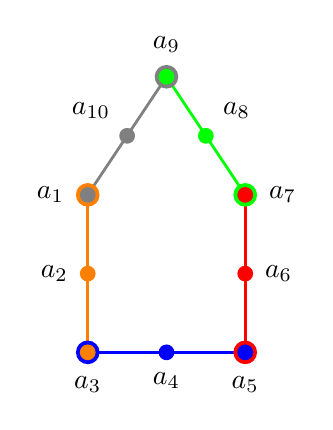
\begin{tikzpicture}  [scale=1]

\tikzstyle{every path}=[line width=1pt]

\newdimen\ms
\ms=0.1cm
\tikzstyle{s1}=[color=red,rectangle,inner sep=3.5]
\tikzstyle{c3}=[circle,inner sep={\ms/8},minimum size=5*\ms]
\tikzstyle{c2}=[circle,inner sep={\ms/8},minimum size=3*\ms]
\tikzstyle{c1}=[circle,inner sep={\ms/8},minimum size=2*\ms]

% Define positions of all observables

\coordinate (a1) at (0,2);
\coordinate (a2) at (0,1);
\coordinate (a3) at (0,0);
\coordinate (a4) at (1,0);
\coordinate (a5) at (2,0);
\coordinate (a6) at (2,1);
\coordinate (a7) at (2,2);
\coordinate (a8) at (1.5,{2+(3.5-2)/2});
\coordinate (a9) at (1,3.5);
\coordinate (a10) at (0.5,{2+(3.5-2)/2});

% draw contexts

\draw [color=orange] (a1) -- (a3);
\draw [color=blue] (a3) -- (a5);
\draw [color=red] (a5) -- (a7);
\draw [color=green] (a7) -- (a9);
\draw [color=gray] (a9) -- (a1);

% draw atoms

\draw (a1) coordinate[c2,fill=orange,label=left:$a_1$];
\draw (a1) coordinate[c1,fill=gray];

\draw (a2) coordinate[c1,fill=orange,label=left:$a_2$];

\draw (a3) coordinate[c2,fill=blue,label=below:$a_3$];
\draw (a3) coordinate[c1,fill=orange];

\draw (a4) coordinate[c1,fill=blue,label=below:$a_4$];

\draw (a5) coordinate[c2,fill=red,label=below:$a_5$];
\draw (a5) coordinate[c1,fill=blue];

\draw (a6) coordinate[c1,fill=red,label=right:$a_6$];

\draw (a7) coordinate[c2,fill=green,label=right:$a_7$];
\draw (a7) coordinate[c1,fill=red];

\draw (a8) coordinate[c1,fill=green,label=above right:$a_8$];

\draw (a9) coordinate[c2,fill=gray,label=above:$a_9$];
\draw (a9) coordinate[c1,fill=green];

\draw (a10) coordinate[c1,fill=gray,label=above left:$a_{10}$];

\end{tikzpicture}
}
&
$
\begin{pmatrix}
1&  0&  0&   1&  0&  1&  0&  1&  0&  0 \\
1&  0&  0&   0&  1&  0&  0&  1&  0&  0\\
1&  0&  0&   1&  0&  0&  1&  0&  0&  0\\
0&  0&  1&    0&  0&  1&  0&  1&  0& 1\\
0&  0&  1&    0&  0&  0&  1&  0&  0& 1\\
0&  0&  1&    0&  0&  1&  0&  0&  1&  0\\
0&  1&  0&   0&  1&  0&  0&  1&  0& 1\\
0&  1&  0&   0&  1&  0&  0&  0&  1&  0\\
0&  1&  0&   1&  0&  0&  1&  0&  0& 1\\
0&  1  &0&   1&  0&  1&  0&  0&  1&  0\\
0&  1&  0&   1&  0&  1&  0&  1&  0& 1 \\
\end{pmatrix}
$
&
\raisebox{-2cm}{
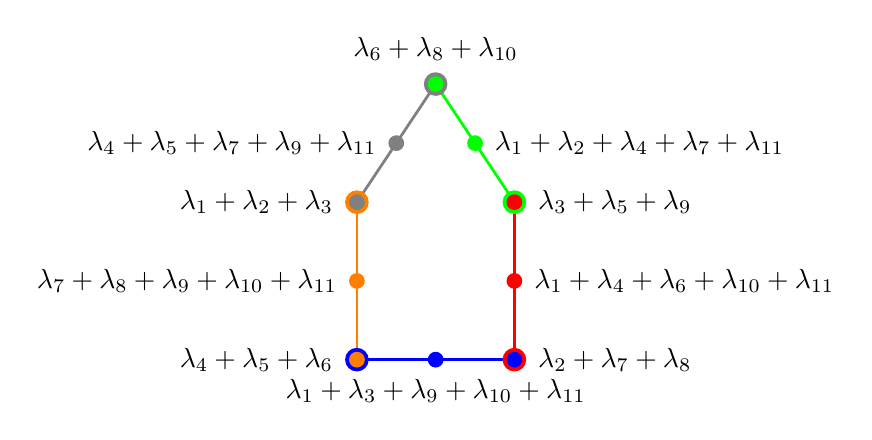
\begin{tikzpicture}  [scale=1]

\tikzstyle{every path}=[line width=1pt]

\newdimen\ms
\ms=0.1cm
\tikzstyle{s1}=[color=red,rectangle,inner sep=3.5]
\tikzstyle{c3}=[circle,inner sep={\ms/8},minimum size=5*\ms]
\tikzstyle{c2}=[circle,inner sep={\ms/8},minimum size=3*\ms]
\tikzstyle{c1}=[circle,inner sep={\ms/8},minimum size=2*\ms]

% Define positions of all observables

\coordinate (a1) at (0,2);
\coordinate (a2) at (0,1);
\coordinate (a3) at (0,0);
\coordinate (a4) at (1,0);
\coordinate (a5) at (2,0);
\coordinate (a6) at (2,1);
\coordinate (a7) at (2,2);
\coordinate (a8) at (1.5,{2+(3.5-2)/2});
\coordinate (a9) at (1,3.5);
\coordinate (a10) at (0.5,{2+(3.5-2)/2});

% draw contexts

\draw [color=orange] (a1) -- (a3);
\draw [color=blue] (a3) -- (a5);
\draw [color=red] (a5) -- (a7);
\draw [color=green] (a7) -- (a9);
\draw [color=gray] (a9) -- (a1);

% draw atoms

\draw (a1) coordinate[c2,fill=orange,label=left:$\lambda_{1} + \lambda_{2} + \lambda_{3}$];
\draw (a1) coordinate[c1,fill=gray];

\draw (a2) coordinate[c1,fill=orange,label=left:$\lambda_{7} + \lambda_{8} + \lambda_{9} + \lambda_{10} + \lambda_{11}$];

\draw (a3) coordinate[c2,fill=blue,label=left:$\lambda_{4} + \lambda_{5} + \lambda_{6}$];
\draw (a3) coordinate[c1,fill=orange];

\draw (a4) coordinate[c1,fill=blue,label=below:$\lambda_{1} + \lambda_{3} + \lambda_{9} + \lambda_{10} + \lambda_{11}$];

\draw (a5) coordinate[c2,fill=red,label=right:$\lambda_{2} + \lambda_{7} + \lambda_{8}$];
\draw (a5) coordinate[c1,fill=blue];

\draw (a6) coordinate[c1,fill=red,label=right:$\lambda_{1} + \lambda_{4} + \lambda_{6} + \lambda_{10} + \lambda_{11}$];

\draw (a7) coordinate[c2,fill=green,label=right:$\lambda_{3} + \lambda_{5} + \lambda_{9}$];
\draw (a7) coordinate[c1,fill=red];

\draw (a8) coordinate[c1,fill=green,label=right:$\lambda_{1} + \lambda_{2} + \lambda_{4} + \lambda_{7} + \lambda_{11}$];

\draw (a9) coordinate[c2,fill=gray,label=above:$\lambda_{6} + \lambda_{8} + \lambda_{10}$];
\draw (a9) coordinate[c1,fill=green];

\draw (a10) coordinate[c1,fill=gray,label=left:$\lambda_{4} + \lambda_{5} + \lambda_{7} + \lambda_{9} + \lambda_{11}$];

\end{tikzpicture}
}
\end{tabular}
}
\end{center}
The sum of the probabilities of the ``intertwining'' observables
$a_1$,
$a_3$,
$a_5$,
$a_7$,
$a_9$---no hull computation is required for this ad hoc estimate---yields the
Bub {\&} Stairs inequality
DOI \href{https://doi.org/10.1007/s10701-009-9307-8}{10.1007/s10701-009-9307-8}:
\[
\lambda_{1} +
2\lambda_{2} +
2\lambda_{3} +
\lambda_{4} +
2\lambda_{5} +
2\lambda_{6} +
\lambda_{7} +
2\lambda_{8} +
\lambda_{9} +
\lambda_{10}  \le 2 \sum_{i=1}^{11}\lambda_i= 2
.\]
\end{frame}



%%%%%%%%%%%%%%%%%%%%%%%%%%%%%%%%%%%%%%%%%%%%%%%%%%%%%%%%%%%%%%%%%%%%%%%%%%%%%%%%%%%%%%%%%%%%%%%%%%%%%%%%%%%%%%%%%%

\begin{frame}[shrink=2]
\frametitle{Five cyclically intertwining contexts: affine shifted values}

Consider now, with Klyachko, Can, Binicioglu, and  Shumovsky
DOI \href{https://doi.org/10.1103/PhysRevLett.101.020403}{10.1103/PhysRevLett.101.020403},
the affine shifted value assignments:
\[
v(a_i) \rightarrow A_1 = 2 v(a_i) - 1
,
\]
or, more explicitly,
\[
v=0 \mapsto A=-1
\text{ and }
v=1 \mapsto A=1.
\]
The associated ``shifted'' Travis matrix is the original one with $0$s substituted by $-1$s.
\\
$\;$\\
Consider the ``bouquet'' of joint probabilities (only joint observables contribute and are thus
\colorbox{yellow}{\textcolor{blue}{marked blue on yellow}}):
\[
\begin{split}
\{
A_1,
A_2,
A_3,
A_4,
A_5,
A_6,
A_7,
A_8,
A_9,
A_{10},
\colorbox{yellow}{\textcolor{blue}{$A_{13}=A_1A_3$}} ,
\\
\colorbox{yellow}{\textcolor{blue}{$A_{35}=A_3A_5$}} ,
\colorbox{yellow}{\textcolor{blue}{$A_{57}=A_5A_7$}} ,
\colorbox{yellow}{\textcolor{blue}{$A_{79}=A_7A_9$}} ,
\colorbox{yellow}{\textcolor{blue}{$A_{91}=A_9A_1$}}
\}
\end{split}
.\]

\end{frame}


%%%%%%%%%%%%%%%%%%%%%%%%%%%%%%%%%%%%%%%%%%%%%%%%%%%%%%%%%%%%%%%%%%%%%%%%%%%%%%%%%%%%%%%%%%%%%%%%%%%%%%%%%%%%%%%%%%

\begin{frame}[shrink=2]
\frametitle{Five cyclically intertwining contexts: affine shifted values cntd.}

The affine shifted Travis matrix then is (please check yourself ;-):
\begin{center}
\resizebox{.75\textwidth}{!}{
$
\begin{pmatrix}
  1  & -1  & -1  &  1  & -1  &  1  & -1  &  1  & -1  & -1 &     \colorbox{yellow}{\textcolor{blue}{$   -1 $}}&\colorbox{yellow}{\textcolor{blue}{$   1 $}}&\colorbox{yellow}{\textcolor{blue}{$   1 $}}&\colorbox{yellow}{\textcolor{blue}{$   1 $}}&\colorbox{yellow}{\textcolor{blue}{$  -1 $}} \\
  1  & -1  & -1  & -1  &  1  & -1  & -1  &  1  & -1  & -1 &     \colorbox{yellow}{\textcolor{blue}{$   -1 $}}&\colorbox{yellow}{\textcolor{blue}{$  -1 $}}&\colorbox{yellow}{\textcolor{blue}{$  -1 $}}&\colorbox{yellow}{\textcolor{blue}{$   1 $}}&\colorbox{yellow}{\textcolor{blue}{$  -1 $}} \\
  1  & -1  & -1  &  1  & -1  & -1  &  1  & -1  & -1  & -1 &     \colorbox{yellow}{\textcolor{blue}{$   -1 $}}&\colorbox{yellow}{\textcolor{blue}{$   1 $}}&\colorbox{yellow}{\textcolor{blue}{$  -1 $}}&\colorbox{yellow}{\textcolor{blue}{$  -1 $}}&\colorbox{yellow}{\textcolor{blue}{$  -1 $}} \\
 -1  & -1  &  1  & -1  & -1  &  1  & -1  &  1  & -1  &  1 &     \colorbox{yellow}{\textcolor{blue}{$   -1 $}}&\colorbox{yellow}{\textcolor{blue}{$  -1 $}}&\colorbox{yellow}{\textcolor{blue}{$   1 $}}&\colorbox{yellow}{\textcolor{blue}{$   1 $}}&\colorbox{yellow}{\textcolor{blue}{$   1 $}} \\
 -1  & -1  &  1  & -1  & -1  & -1  &  1  & -1  & -1  &  1 &     \colorbox{yellow}{\textcolor{blue}{$   -1 $}}&\colorbox{yellow}{\textcolor{blue}{$  -1 $}}&\colorbox{yellow}{\textcolor{blue}{$  -1 $}}&\colorbox{yellow}{\textcolor{blue}{$  -1 $}}&\colorbox{yellow}{\textcolor{blue}{$   1 $}} \\
 -1  & -1  &  1  & -1  & -1  &  1  & -1  & -1  &  1  & -1 &     \colorbox{yellow}{\textcolor{blue}{$   -1 $}}&\colorbox{yellow}{\textcolor{blue}{$  -1 $}}&\colorbox{yellow}{\textcolor{blue}{$   1 $}}&\colorbox{yellow}{\textcolor{blue}{$  -1 $}}&\colorbox{yellow}{\textcolor{blue}{$  -1 $}} \\
 -1  &  1  & -1  & -1  &  1  & -1  & -1  &  1  & -1  &  1 &     \colorbox{yellow}{\textcolor{blue}{$    1 $}}&\colorbox{yellow}{\textcolor{blue}{$  -1 $}}&\colorbox{yellow}{\textcolor{blue}{$  -1 $}}&\colorbox{yellow}{\textcolor{blue}{$   1 $}}&\colorbox{yellow}{\textcolor{blue}{$   1 $}} \\
 -1  &  1  & -1  & -1  &  1  & -1  & -1  & -1  &  1  & -1 &     \colorbox{yellow}{\textcolor{blue}{$    1 $}}&\colorbox{yellow}{\textcolor{blue}{$  -1 $}}&\colorbox{yellow}{\textcolor{blue}{$  -1 $}}&\colorbox{yellow}{\textcolor{blue}{$  -1 $}}&\colorbox{yellow}{\textcolor{blue}{$  -1 $}} \\
 -1  &  1  & -1  &  1  & -1  & -1  &  1  & -1  & -1  &  1 &     \colorbox{yellow}{\textcolor{blue}{$    1 $}}&\colorbox{yellow}{\textcolor{blue}{$   1 $}}&\colorbox{yellow}{\textcolor{blue}{$  -1 $}}&\colorbox{yellow}{\textcolor{blue}{$  -1 $}}&\colorbox{yellow}{\textcolor{blue}{$   1 $}} \\
 -1  &  1  & -1  &  1  & -1  &  1  & -1  & -1  &  1  & -1 &     \colorbox{yellow}{\textcolor{blue}{$    1 $}}&\colorbox{yellow}{\textcolor{blue}{$   1 $}}&\colorbox{yellow}{\textcolor{blue}{$   1 $}}&\colorbox{yellow}{\textcolor{blue}{$  -1 $}}&\colorbox{yellow}{\textcolor{blue}{$  -1 $}} \\
 -1  &  1  & -1  &  1  & -1  &  1  & -1  &  1  & -1  &  1 &     \colorbox{yellow}{\textcolor{blue}{$    1 $}}&\colorbox{yellow}{\textcolor{blue}{$   1 $}}&\colorbox{yellow}{\textcolor{blue}{$   1 $}}&\colorbox{yellow}{\textcolor{blue}{$   1 $}}&\colorbox{yellow}{\textcolor{blue}{$   1 $}} \\
\end{pmatrix}
$
}
\end{center}

Input for the Hull computation:

\begin{flushleft}
{\tiny
\textcolor{Gray}{${\tt import \; cdd}$}\\
${\tt mat = cdd.Matrix([}$\\
${\tt [1, \colorbox{yellow}{\textcolor{blue}{   -1 }}, \colorbox{yellow}{\textcolor{blue}{   1 }}, \colorbox{yellow}{\textcolor{blue}{   1 }}, \colorbox{yellow}{\textcolor{blue}{   1 }}, \colorbox{yellow}{\textcolor{blue}{  -1 }}  ],}$\\
${\tt [1, \colorbox{yellow}{\textcolor{blue}{   -1 }}, \colorbox{yellow}{\textcolor{blue}{  -1 }}, \colorbox{yellow}{\textcolor{blue}{  -1 }}, \colorbox{yellow}{\textcolor{blue}{   1 }}, \colorbox{yellow}{\textcolor{blue}{  -1 }}  ],}$\\
${\tt [1, \colorbox{yellow}{\textcolor{blue}{   -1 }}, \colorbox{yellow}{\textcolor{blue}{   1 }}, \colorbox{yellow}{\textcolor{blue}{  -1 }}, \colorbox{yellow}{\textcolor{blue}{  -1 }}, \colorbox{yellow}{\textcolor{blue}{  -1 }}  ],}$\\
${\tt [1, \colorbox{yellow}{\textcolor{blue}{   -1 }}, \colorbox{yellow}{\textcolor{blue}{  -1 }}, \colorbox{yellow}{\textcolor{blue}{   1 }}, \colorbox{yellow}{\textcolor{blue}{   1 }}, \colorbox{yellow}{\textcolor{blue}{   1 }}  ],}$\\
${\tt [1, \colorbox{yellow}{\textcolor{blue}{   -1 }}, \colorbox{yellow}{\textcolor{blue}{  -1 }}, \colorbox{yellow}{\textcolor{blue}{  -1 }}, \colorbox{yellow}{\textcolor{blue}{  -1 }}, \colorbox{yellow}{\textcolor{blue}{   1 }}  ],}$\\
${\tt [1, \colorbox{yellow}{\textcolor{blue}{   -1 }}, \colorbox{yellow}{\textcolor{blue}{  -1 }}, \colorbox{yellow}{\textcolor{blue}{   1 }}, \colorbox{yellow}{\textcolor{blue}{  -1 }}, \colorbox{yellow}{\textcolor{blue}{  -1 }}  ],}$\\
${\tt [1, \colorbox{yellow}{\textcolor{blue}{    1 }}, \colorbox{yellow}{\textcolor{blue}{  -1 }}, \colorbox{yellow}{\textcolor{blue}{  -1 }}, \colorbox{yellow}{\textcolor{blue}{   1 }}, \colorbox{yellow}{\textcolor{blue}{   1 }}  ],}$\\
${\tt [1, \colorbox{yellow}{\textcolor{blue}{    1 }}, \colorbox{yellow}{\textcolor{blue}{  -1 }}, \colorbox{yellow}{\textcolor{blue}{  -1 }}, \colorbox{yellow}{\textcolor{blue}{  -1 }}, \colorbox{yellow}{\textcolor{blue}{  -1 }}  ],}$\\
${\tt [1, \colorbox{yellow}{\textcolor{blue}{    1 }}, \colorbox{yellow}{\textcolor{blue}{   1 }}, \colorbox{yellow}{\textcolor{blue}{  -1 }}, \colorbox{yellow}{\textcolor{blue}{  -1 }}, \colorbox{yellow}{\textcolor{blue}{   1 }}  ],}$\\
${\tt [1, \colorbox{yellow}{\textcolor{blue}{    1 }}, \colorbox{yellow}{\textcolor{blue}{   1 }}, \colorbox{yellow}{\textcolor{blue}{   1 }}, \colorbox{yellow}{\textcolor{blue}{  -1 }}, \colorbox{yellow}{\textcolor{blue}{  -1 }}  ],}$\\
${\tt [1, \colorbox{yellow}{\textcolor{blue}{    1 }}, \colorbox{yellow}{\textcolor{blue}{   1 }}, \colorbox{yellow}{\textcolor{blue}{   1 }}, \colorbox{yellow}{\textcolor{blue}{   1 }}, \colorbox{yellow}{\textcolor{blue}{   1 }}  ]])}$\\
${\tt poly = cdd.Polyhedron(mat)}$\\
${\tt ine = poly.get\_inequalities()}$\\
${\tt print(ine)}$
}
\end{flushleft}


\end{frame}

%%%%%%%%%%%%%%%%%%%%%%%%%%%%%%%%%%%%%%%%%%%%%%%%%%%%%%%%%%%%%%%%%%%%%%%%%%%%%%%%%%%%%%%%%%%%%%%%%%%%%%%%%%%%%%%%%%

\begin{frame}[shrink=2]
 \frametitle{Hull computation for the affine shifted values of propositions
arranged in five cyclically intertwining contexts: the ``pentagram inequality''}


{\scriptsize
${\tt H-representation }$\\
${\tt begin                        }$\\
${\tt  \;    11 \; 6 \;  rational                           }$\\
${\tt        1   \;       0   \;        0    \;       0      \;      1     \;      0           }$\\
${\tt        1   \;       0   \;        0    \;       0      \;     0      \;      1           }$\\
${\tt        1   \;       0   \;         1   \;        0     \;      0     \;      0           }$\\
${\tt        3   \;   1       \;     1       \;     1        \;    1       \;     1            }$\\
$\qquad \textcolor{applegreen}{\Rightarrow  3 \ge -A_{13}-A_{35}-A_{57}-A_{79}-A_{91} }$\\
$\qquad \textcolor{applegreen}{\Rightarrow    A_{13}+A_{35}+A_{57}+A_{79}+A_{91}\ge - 3}$\\
${\tt        1   \;        1  \;         0   \;        0     \;      0     \;      0           }$\\
${\tt        1   \;       0   \;        0    \;        1     \;      0     \;      0           }$\\
${\tt        1   \;        1  \;         -1  \;          1   \;        -1  \;         -1       }$\\
${\tt        1   \;       -1  \;          1  \;         -1   \;        -1  \;          1       }$\\
${\tt        1   \;        1  \;         -1  \;         -1   \;         1  \;         -1       }$\\
${\tt        1   \;       -1  \;          1  \;         -1   \;         1  \;         -1       }$\\
${\tt        1   \;       -1  \;         -1  \;          1   \;        -1  \;          1       }$\\
${\tt end     }$
}

The art here, as in the Bub-Stairs inequality, and indeed, all Boole-Bell type inequalities, is to figure out
``bouquets'' of (joint) probabilities that are violated for at least some quantum states.





\end{frame}

\section{Insert: Cabello's ``contextual inequalities'' are not from Hull computations}

%%%%%%%%%%%%%%%%%%%%%%%%%%%%%%%%%%%%%%%%%%%%%%%%%%%%%%%%%%%%%%%%%%%%%%%%%%%%%%%%%%%%%%%%%%%%%%%%%%%%%%%%%%%%%%%%%%

\begin{frame}
\begin{center}
{\large {\color{purple}$\;$}}
\end{center}

                                                    \vspace{1.15cm}

\centerline{\Large {\color{applegreen}{\color{blue}\decofourleft} \begin{tabular}{c}{\it Leaving the hull problem}\\{\it for deriving classical bounds on probabilities~$\ldots$}\end{tabular}\hspace{.15cm} {\color{blue}\decofourright}}}

                                                    \vspace{1.15cm}
\begin{center}
{\large {\color{blue} $\;$}}
\end{center}

\end{frame}

\begin{frame}%[shrink=10]
 \frametitle{Insert: Cabello's ad hoc ``contextual inequalities'' are not from hull computations}


One can ``ease'' the rules for the two-valued states and just consider \textbf{any} binary value assignment---provided that it is not
context dependent---so this value assignment should be global but otherwise arbitrary.
Cabello did a respective brute-force or exhaustive search computation in
DOI \href{https://doi.org/10.1016/0375-9601(96)00134-X}{10.1016/0375-9601(96)00134-X},
for a Kochen-Specker type logical structure
introduced
by
Cabello, Estebaranz, and Garc{\'{i}}a-Alcaine
in
DOI \href{https://doi.org/10.1016/0375-9601(96)00134-X}{10.1016/0375-9601(96)00134-X},
which has no ``classical'' two-valued state.

This logic involves 18 binary observables in 9 contexts
and thus results in $2^{18} = 262144$ vertices.
Cabello in
DOI \href{https://doi.org/10.1103/PhysRevLett.101.210401}{10.1103/PhysRevLett.101.210401}
considered the 9 (from the 9 contexts involved) 4th order joint expectations corresponding to the products of all binary-$\{-1,1\}$
observables in the 9 contexts involved.

\end{frame}

\section{Insert: Cabello's ``contextual inequalities'' cntd.}

\begin{frame}%[shrink=10]
 \frametitle{Insert: Cabello's ``contextual inequalities'' are not from hull computations}

A  brute-force or exhaustive search computation finds that, classically,
if all 9 (from the 9 contexts involved)
such products from the 4th order joint expectations are added together, the minimum is $-7$.
 Indeed, this can be readily checked (please do with a computer program ;-):
there are 9216 of 262144 value assignments rendering $-7$, and no $-8$ or $-9$ instances.

However, quantum mechanically, a straightforward calculation shows that, for binary-$\{-1,1\}$ observables
$2\vert a_i\rangle \langle a_i \vert - \mathbb{1}$, and for vectors $\vert a_i\rangle $ of an arbitrary orthomodular basis,
$\prod_{i=1}^4 \big( 2\vert a_i\rangle \langle a_i \vert - \mathbb{1} \big)=
-2 \left(  \sum_{i=1}^4 \vert a_i\rangle \langle a_i \vert\right)   + \mathbb{1} = (-2+1) \mathbb{1}= - \mathbb{1}$.
Therefore,
quantum mechanics requires these 4th order joint expectations to be always $-9$, regardless of the state.

It is important to emphasize that this is no hull computation,
and the bound from below of $-7$ is no Boole-type inequality.

\end{frame}


\begin{frame}
\begin{center}
{\large {\color{purple}$\;$}}
\end{center}

                                                    \vspace{1.15cm}

\centerline{\Large {\color{applegreen}{\color{blue}\decofourleft} {\it Quantum gadgets}\hspace{.15cm} {\color{blue}\decofourright}}}

                                                    \vspace{1.15cm}
\begin{center}
{\large {\color{blue} $\;$}}
\end{center}

\end{frame}

\subsection{Seven bi-intertwining contexts with three mutually exclusive observables (``Specker bug''/``cat's cradle'' shaped hypergraph)}

\begin{frame} [shrink=10]
\frametitle{True-implies-false (TIF) gadget: Seven bi-intertwining contexts with three mutually exclusive observables:
``Specker bug''/Pitowsky's ``cat's cradle''}



Kochen {\&} Specker, 1965 DOI \href{https://doi.org/10.1007/978-3-0348-9259-9\_19}{10.1007/978-3-0348-9259-9\_19}
re-discovered and analyzed by various authors:

\resizebox{.95\textwidth}{!}{
\begin{tabular}{ccc}
\raisebox{-2.25cm}{
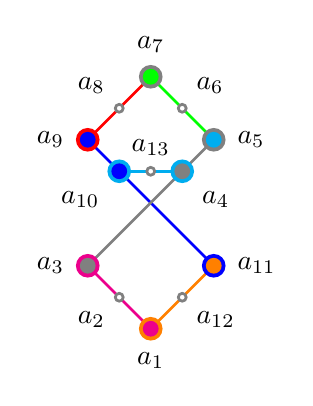
\begin{tikzpicture}  [scale=0.8]

\tikzstyle{every path}=[line width=1pt]

\newdimen\ms
\ms=0.1cm
\tikzstyle{s1}=[color=red,rectangle,inner sep=3.5]
\tikzstyle{c3}=[circle,inner sep={\ms/8},minimum size=5*\ms]
\tikzstyle{c2}=[circle,inner sep={\ms/8},minimum size=3*\ms]
\tikzstyle{c1}=[circle,inner sep={\ms/8},minimum size=2*\ms]
\tikzstyle{cs1}=[circle,inner sep={\ms/8},minimum size=1*\ms]

% Define positions of all observables


\coordinate (a7) at  (1,2);
\coordinate (a5) at (2,1);
\coordinate (a10) at (0.5,0.5);
\coordinate (a11) at (2,-1);
\coordinate (a1) at (1,-2);
\coordinate (a3) at (0,-1);
\coordinate (a4) at (1.5,0.5);
\coordinate (a9) at (0,1);



% draw contexts

\draw [color=orange] (a1) -- (a11)  coordinate[cs1,fill=white,draw=gray,pos=0.5,label=below right:{\color{black}$a_{12}$}] (a12);
\draw [color=blue] (a11) -- (a9);
\draw [color=red] (a9) -- (a7)  coordinate[cs1,fill=white,draw=gray,pos=0.5,label=above left:{\color{black}$a_8$}] (a8);
\draw [color=green] (a7) -- (a5)  coordinate[cs1,fill=white,draw=gray,pos=0.5,label=above right:{\color{black}$a_6$}] (a6);
\draw [color=gray] (a5) -- (a3);
\draw [color=magenta] (a1) -- (a3)  coordinate[cs1,fill=white,draw=gray,pos=0.5,label= below left:{\color{black}$a_2$}] (a2);
\draw [color=cyan] (a10) -- (a4)  coordinate[cs1,fill=white,draw=gray,pos=0.5,label=above:{\color{black}$a_{13}$}] (a13);




% draw atoms

\draw (a1) coordinate[c2,fill=orange,label=below:$a_1$];
\draw (a1) coordinate[c1,fill=magenta];


\draw (a3) coordinate[c2,fill=magenta,label=left:$a_3$];
\draw (a3) coordinate[c1,fill=gray];

\draw (a11) coordinate[c2,fill=blue,label=right:$a_{11}$];
\draw (a11) coordinate[c1,fill=orange];

\draw (a10) coordinate[c2,fill=cyan,label=below left:$a_{10}$];
\draw (a10) coordinate[c1,fill=blue];

\draw (a5) coordinate[c2,fill=gray,label=right:$a_{5}$];
\draw (a5) coordinate[c1,fill=cyan];

\draw (a9) coordinate[c2,fill=red,label=left:$a_9$];
\draw (a9) coordinate[c1,fill=blue];


\draw (a7) coordinate[c2,fill=gray,label=above:$a_7$];
\draw (a7) coordinate[c1,fill=green];

\draw (a4) coordinate[c2,fill=cyan,label=below right:$a_4$];
\draw (a4) coordinate[c1,fill=gray];


\end{tikzpicture}
}
&
{\scriptsize
$
\begin{pmatrix}
\colorbox{yellow}{\textcolor{blue}{$1$}}&0& 0& 1& 0& 1& 0& 0& 1& 0& 0& 0& 0\\
\colorbox{yellow}{\textcolor{blue}{$1$}}&0& 0& 0& 1& 0& 0& 1& 0& 1& 0& 0& 0\\
\colorbox{yellow}{\textcolor{blue}{$1$}}&0& 0& 0& 1& 0& 0& 0& 1& 0& 0& 0& 1\\
0&1& 0& 1& 0& 1& 0& 1& 0& 0& 1& 0& 0\\
0&1& 0& 1& 0& 1& 0& 0& 1& 0& 0& 1& 0\\
0&1& 0& 1& 0& 0& \colorbox{blue}{\textcolor{yellow}{$1$}}& 0& 0& 0& 1& 0& 0\\
0&1& 0& 0& 1& 0& 0& 1& 0& 1& 0& 1& 0\\
0&1& 0& 0& 1& 0& 0& 1& 0& 0& 1& 0& 1\\
0&1& 0& 0& 1& 0& 0& 0& 1& 0& 0& 1& 1\\
0&0& 1& 0& 0& 1& 0& 1& 0& 1& 0& 1& 0\\
0&0& 1& 0& 0& 1& 0& 1& 0& 0& 1& 0& 1\\
0&0& 1& 0& 0& 1& 0& 0& 1& 0& 0& 1& 1\\
0&0& 1& 0& 0& 0& \colorbox{blue}{\textcolor{yellow}{$1$}}& 0& 0& 1& 0& 1& 0\\
0&0& 1& 0& 0& 0& \colorbox{blue}{\textcolor{yellow}{$1$}}& 0& 0& 0& 1& 0& 1\\
\end{pmatrix}
$ }
&
\raisebox{-2.25cm}{
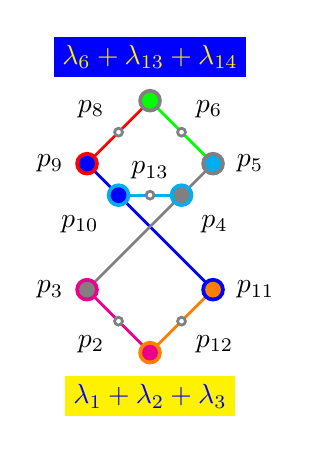
\begin{tikzpicture}  [scale=0.8]

\tikzstyle{every path}=[line width=1pt]

\newdimen\ms
\ms=0.1cm
\tikzstyle{s1}=[color=red,rectangle,inner sep=3.5]
\tikzstyle{c3}=[circle,inner sep={\ms/8},minimum size=5*\ms]
\tikzstyle{c2}=[circle,inner sep={\ms/8},minimum size=3*\ms]
\tikzstyle{c1}=[circle,inner sep={\ms/8},minimum size=2*\ms]
\tikzstyle{cs1}=[circle,inner sep={\ms/8},minimum size=1*\ms]

% Define positions of all observables


\coordinate (a7) at  (1,2);
\coordinate (a5) at (2,1);
\coordinate (a10) at (0.5,0.5);
\coordinate (a11) at (2,-1);
\coordinate (a1) at (1,-2);
\coordinate (a3) at (0,-1);
\coordinate (a4) at (1.5,0.5);
\coordinate (a9) at (0,1);



% draw contexts

\draw [color=orange] (a1) -- (a11)  coordinate[cs1,fill=white,draw=gray,pos=0.5,label=below right:{\color{black}$p_{12}$}] (a12);
\draw [color=blue] (a11) -- (a9);
\draw [color=red] (a9) -- (a7)  coordinate[cs1,fill=white,draw=gray,pos=0.5,label=above left:{\color{black}$p_8$}] (a8);
\draw [color=green] (a7) -- (a5)  coordinate[cs1,fill=white,draw=gray,pos=0.5,label=above right:{\color{black}$p_6$}] (a6);
\draw [color=gray] (a5) -- (a3);
\draw [color=magenta] (a1) -- (a3)  coordinate[cs1,fill=white,draw=gray,pos=0.5,label= below left:{\color{black}$p_2$}] (a2);
\draw [color=cyan] (a10) -- (a4)  coordinate[cs1,fill=white,draw=gray,pos=0.5,label=above:{\color{black}$p_{13}$}] (a13);




% draw atoms

\draw (a1) coordinate[c2,fill=orange,label=below:\colorbox{yellow}{\textcolor{blue}{$\lambda_1+\lambda_2+\lambda_3$}}];
\draw (a1) coordinate[c1,fill=magenta];


\draw (a3) coordinate[c2,fill=magenta,label=left:$p_3$];
\draw (a3) coordinate[c1,fill=gray];

\draw (a11) coordinate[c2,fill=blue,label=right:$p_{11}$];
\draw (a11) coordinate[c1,fill=orange];

\draw (a10) coordinate[c2,fill=cyan,label=below left:$p_{10}$];
\draw (a10) coordinate[c1,fill=blue];

\draw (a5) coordinate[c2,fill=gray,label=right:$p_{5}$];
\draw (a5) coordinate[c1,fill=cyan];

\draw (a9) coordinate[c2,fill=red,label=left:$p_9$];
\draw (a9) coordinate[c1,fill=blue];


\draw (a7) coordinate[c2,fill=gray,label=above:\colorbox{blue}{\textcolor{yellow}{$\lambda_6+\lambda_{13}+\lambda_{14}$}}];
\draw (a7) coordinate[c1,fill=green];

\draw (a4) coordinate[c2,fill=cyan,label=below right:$p_4$];
\draw (a4) coordinate[c1,fill=gray];


\end{tikzpicture}
}
\end{tabular}
}

This ``Specker bug'' (Specker's ``K\"afer'') can be employed as a classical (non-contextual) true-implies-false (TIF) gadget, as
the two ``terminal points'' $a_1$ and $a_7$ cannot both be ``true'' (value 1) at the same time.
Nevertheless one can be true (have value 1) and the other one false (value 0).
Also they can both be false (value 0): their respective probabilities
\colorbox{yellow}{\textcolor{blue}{$\lambda_1+\lambda_2+\lambda_3$}}
and
\colorbox{blue}{\textcolor{yellow}{$\lambda_6+\lambda_{13}+\lambda_{14}$}}
are mutually exclusive!


\end{frame}

%%%%%%%%%%%%%%%%%%%%%%%%%%%%%%%%%%%%%%%%%%%%%%%%%%%%%%%%%%%%%%%%%%%%%%%%%%%%%%%%%%%%%%%%%%%%%%%%%%%%%%%%%%%%%%%%%%%%%%%%%%%%%%%%%%

\begin{frame}%[shrink=5]
\frametitle{Specker bug as TIF gadget continued: proof by contradiction}

From DOI \href{https://doi.org/10.1103/PhysRevA.103.022204}{10.1103/PhysRevA.103.022204}

\begin{center}
\resizebox{1\textwidth}{!}{
\begin{tabular}{ c c c c c c}
\resizebox{.33\textwidth}{!}{%
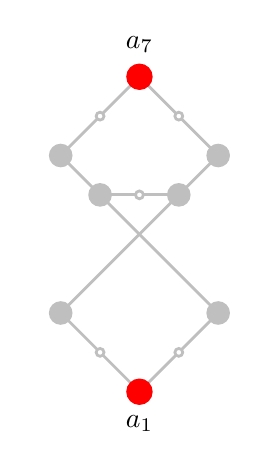
\begin{tikzpicture}  [scale=1]

\tikzstyle{every path}=[line width=1pt]

\newdimen\ms
\ms=0.1cm
\tikzstyle{s1}=[color=lightgray,rectangle,inner sep=3.5]
\tikzstyle{c3}=[circle,inner sep={\ms/8},minimum size=5*\ms]
\tikzstyle{c2}=[circle,inner sep={\ms/8},minimum size=3*\ms]
\tikzstyle{c1}=[circle,inner sep={\ms/8},minimum size=2*\ms]
\tikzstyle{cs1}=[circle,inner sep={\ms/8},minimum size=1*\ms]

% Define positions of all observables

\coordinate (a8) at  (1,2);
\coordinate (a7) at (2,1);
\coordinate (a4) at (0.5,0.5);
\coordinate (a3) at (2,-1);
\coordinate (a1) at (1,-2);
\coordinate (a2) at (0,-1);
\coordinate (a5) at (1.5,0.5);
\coordinate (a6) at (0,1);

% draw contexts

\draw [color=lightgray] (a1) -- (a3)  coordinate[cs1,fill=white,draw=lightgray,pos=0.5] (2);
\draw [color=lightgray] (a3) -- (a6);
\draw [color=lightgray] (a6) -- (a8)  coordinate[cs1,fill=white,draw=lightgray,pos=0.5] (7);
\draw [color=lightgray] (a7) -- (a8)  coordinate[cs1,fill=white,draw=lightgray,pos=0.5] (3);
\draw [color=lightgray] (a2) -- (a7);
\draw [color=lightgray] (a2) -- (a1)  coordinate[cs1,fill=white,draw=lightgray,pos=0.5] (10);
\draw [color=lightgray] (a4) -- (a5)  coordinate[cs1,fill=white,draw=lightgray,pos=0.5] (13);

% draw atoms

\draw (a1) coordinate[c2,fill=red,draw=red,label=below:$a_1$];
\draw (a2) coordinate[c2,fill=lightgray,label=left:$ $];
\draw (a3) coordinate[c2,fill=lightgray,label=right:$ $];
\draw (a4) coordinate[c2,fill=lightgray,label=left:$ $];
\draw (a5) coordinate[c2,fill=lightgray,label=right:$ $];
\draw (a6) coordinate[c2,fill=lightgray,label=left:$ $];
\draw (a7) coordinate[c2,fill=lightgray,label=right:$ $];
\draw (a8) coordinate[c2,fill=red,draw=red,label=above:$a_7$];

\end{tikzpicture}
}
\quad
\quad
&
\quad
\quad
\resizebox{.33\textwidth}{!}{%
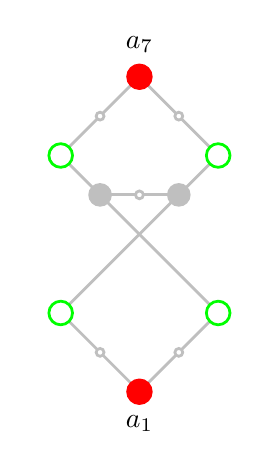
\begin{tikzpicture}  [scale=1]
\tikzstyle{every path}=[line width=1pt]

\newdimen\ms
\ms=0.1cm
\tikzstyle{s1}=[color=lightgray,rectangle,inner sep=3.5]
\tikzstyle{c3}=[circle,inner sep={\ms/8},minimum size=5*\ms]
\tikzstyle{c2}=[circle,inner sep={\ms/8},minimum size=3*\ms]
\tikzstyle{c1}=[circle,inner sep={\ms/8},minimum size=2*\ms]
\tikzstyle{cs1}=[circle,inner sep={\ms/8},minimum size=1*\ms]

% Define positions of all observables

\coordinate (a8) at  (1,2);
\coordinate (a7) at (2,1);
\coordinate (a4) at (0.5,0.5);
\coordinate (a3) at (2,-1);
\coordinate (a1) at (1,-2);
\coordinate (a2) at (0,-1);
\coordinate (a5) at (1.5,0.5);
\coordinate (a6) at (0,1);

% draw contexts

\draw [color=lightgray] (a1) -- (a3)  coordinate[cs1,fill=white,draw=lightgray,pos=0.5] (2);
\draw [color=lightgray] (a3) -- (a6);
\draw [color=lightgray] (a6) -- (a8)  coordinate[cs1,fill=white,draw=lightgray,pos=0.5] (7);
\draw [color=lightgray] (a7) -- (a8)  coordinate[cs1,fill=white,draw=lightgray,pos=0.5] (3);
\draw [color=lightgray] (a2) -- (a7);
\draw [color=lightgray] (a2) -- (a1)  coordinate[cs1,fill=white,draw=lightgray,pos=0.5] (10);
\draw [color=lightgray] (a4) -- (a5)  coordinate[cs1,fill=white,draw=lightgray,pos=0.5] (13);

% draw atoms

\draw (a1) coordinate[c2,fill=red,draw=red,label=below:$a_1$];
\draw (a2) coordinate[c2,fill=white,draw=green,label=left:$ $];
\draw (a3) coordinate[c2,fill=white,draw=green,label=right:$ $];
\draw (a4) coordinate[c2,fill=lightgray,label=left:$ $];
\draw (a5) coordinate[c2,fill=lightgray,label=right:$ $];
\draw (a6) coordinate[c2,fill=white,draw=green,label=left:$ $];
\draw (a7) coordinate[c2,fill=white,draw=green,label=right:$ $];
\draw (a8) coordinate[c2,fill=red,draw=red,label=above:$a_7$];

\end{tikzpicture}
}
\quad
\quad
&
\quad
\quad
\resizebox{.33\textwidth}{!}{%
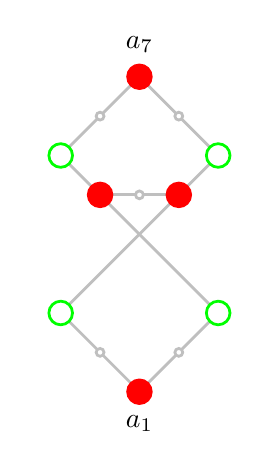
\begin{tikzpicture}  [scale=1]
\tikzstyle{every path}=[line width=1pt]

\newdimen\ms
\ms=0.1cm
\tikzstyle{s1}=[color=lightgray,rectangle,inner sep=3.5]
\tikzstyle{c3}=[circle,inner sep={\ms/8},minimum size=5*\ms]
\tikzstyle{c2}=[circle,inner sep={\ms/8},minimum size=3*\ms]
\tikzstyle{c1}=[circle,inner sep={\ms/8},minimum size=2*\ms]
\tikzstyle{cs1}=[circle,inner sep={\ms/8},minimum size=1*\ms]

% Define positions of all observables

\coordinate (a8) at  (1,2);
\coordinate (a7) at (2,1);
\coordinate (a4) at (0.5,0.5);
\coordinate (a3) at (2,-1);
\coordinate (a1) at (1,-2);
\coordinate (a2) at (0,-1);
\coordinate (a5) at (1.5,0.5);
\coordinate (a6) at (0,1);

% draw contexts

\draw [color=lightgray] (a1) -- (a3)  coordinate[cs1,fill=white,draw=lightgray,pos=0.5] (2);
\draw [color=lightgray] (a3) -- (a6);
\draw [color=lightgray] (a6) -- (a8)  coordinate[cs1,fill=white,draw=lightgray,pos=0.5] (7);
\draw [color=lightgray] (a7) -- (a8)  coordinate[cs1,fill=white,draw=lightgray,pos=0.5] (3);
\draw [color=lightgray] (a2) -- (a7);
\draw [color=lightgray] (a2) -- (a1)  coordinate[cs1,fill=white,draw=lightgray,pos=0.5] (10);
\draw [color=lightgray] (a4) -- (a5)  coordinate[cs1,fill=white,draw=lightgray,pos=0.5] (13);

% draw atoms

\draw (a1) coordinate[c2,fill=red,draw=red,label=below:$a_1$];
\draw (a2) coordinate[c2,fill=white,draw=green,label=left:$ $];
\draw (a3) coordinate[c2,fill=white,draw=green,label=right:$ $];
\draw (a4) coordinate[c2,fill=red,draw=red,label=left:$ $];
\draw (a5) coordinate[c2,fill=red,draw=red,label=right:$ $];
\draw (a6) coordinate[c2,fill=white,draw=green,label=left:$ $];
\draw (a7) coordinate[c2,fill=white,draw=green,label=right:$ $];
\draw (a8) coordinate[c2,fill=red,draw=red,label=above:$a_7$];

\end{tikzpicture}
}
\\
``wrong'' assumption: both &consequence&``wrong'' consequence: only one atom
\\
terminals $a_1$ and $a_7$ have value 1&&in a context can have value 1
\end{tabular}
}
\end{center}
Note: TIF gadgets are symmetric with respect to an exchange of their terminal points!
\end{frame}

%%%%%%%%%%%%%%%%%%%%%%%%%%%%%%%%%%%%%%%%%%%%%%%%%%%%%%%%%%%%%%%%%%%%%%%%%%%%%%%%%%%%%%%%%%%%%%%%%%%%%%%%%%%%%%%%%%

\begin{frame}%[shrink=2]
\frametitle{Specker bug as TIF gadget continued: quantum predictions}

\begin{center}
\resizebox{.43\textwidth}{!}{%
\begin{tikzpicture}  [scale=1]

\tikzstyle{every path}=[line width=1pt]

\newdimen\ms
\ms=0.1cm
\tikzstyle{s1}=[color=red,rectangle,inner sep=3.5]
\tikzstyle{c3}=[circle,inner sep={\ms/8},minimum size=5*\ms]
\tikzstyle{c2}=[circle,inner sep={\ms/8},minimum size=3*\ms]
\tikzstyle{c1}=[circle,inner sep={\ms/8},minimum size=2*\ms]
\tikzstyle{cs1}=[circle,inner sep={\ms/8},minimum size=1*\ms]

% Define positions of all observables


\coordinate (a7) at  (1,2);
\coordinate (a5) at (2,1);
\coordinate (a10) at (0.5,0.5);
\coordinate (a11) at (2,-1);
\coordinate (a1) at (1,-2);
\coordinate (a3) at (0,-1);
\coordinate (a4) at (1.5,0.5);
\coordinate (a9) at (0,1);



% draw contexts

\draw [color=orange] (a1) -- (a11)  coordinate[cs1,fill=white,draw=gray,pos=0.5,label=below right:{\scriptsize \color{black}$\begin{pmatrix}0,1,\sqrt{3}\end{pmatrix}$}] (a12);
\draw [color=blue] (a11) -- (a9);
\draw [color=red] (a9) -- (a7)  coordinate[cs1,fill=white,draw=gray,pos=0.5,label=above left:{\scriptsize \color{black}$\begin{pmatrix}-2\sqrt{2},\sqrt{2},-3\sqrt{3}\end{pmatrix}$}] (a8);
\draw [color=green] (a7) -- (a5)  coordinate[cs1,fill=white,draw=gray,pos=0.5,label=above right:{\scriptsize \color{black}$\begin{pmatrix}2\sqrt{2},-1,-3\sqrt{3}\end{pmatrix}$}] (a6);
\draw [color=gray] (a5) -- (a3);
\draw [color=magenta] (a1) -- (a3)  coordinate[cs1,fill=white,draw=gray,pos=0.5,label= below left:{\scriptsize \color{black}$\begin{pmatrix}0, -1, \sqrt{3}]\end{pmatrix}$}] (a2);
\draw [color=cyan] (a10) -- (a4)  coordinate[cs1,fill=white,draw=gray,pos=0.5,label=above:{\tiny \color{black}$\begin{pmatrix}2,-2\sqrt{2},0\end{pmatrix}$}] (a13);




% draw atoms

 \draw (a1) coordinate[c2,fill=orange,label=below:{\colorbox{yellow}{\textcolor{blue}{$\begin{pmatrix}1,0,0\end{pmatrix}$}}}];
 \draw (a1) coordinate[c1,fill=magenta];


\draw (a3) coordinate[c2,fill=magenta,label=left:{$\begin{pmatrix}0,\sqrt{3},1\end{pmatrix}$}];
\draw (a3) coordinate[c1,fill=gray];

\draw (a11) coordinate[c2,fill=blue,label=right:{$\begin{pmatrix}0,\sqrt{3},-1\end{pmatrix}$}];
\draw (a11) coordinate[c1,fill=orange];

\draw (a10) coordinate[c2,fill=cyan,label=below left:{$\begin{pmatrix}\sqrt{2},1,\sqrt{3}\end{pmatrix}$}];
\draw (a10) coordinate[c1,fill=blue];

\draw (a5) coordinate[c2,fill=gray,label=right:{$\begin{pmatrix}-2\sqrt{2},1,-\sqrt{3}\end{pmatrix}$}];
\draw (a5) coordinate[c1,fill=cyan];

\draw (a9) coordinate[c2,fill=red,label=left:{$\begin{pmatrix}-2\sqrt{2},1,\sqrt{3}\end{pmatrix}$}];
\draw (a9) coordinate[c1,fill=blue];


\draw (a7) coordinate[c2,fill=gray,label=above:{\colorbox{blue}{\textcolor{yellow}{$\begin{pmatrix}1,2\sqrt{2},0\end{pmatrix}$}}}];
\draw (a7) coordinate[c1,fill=green];

\draw (a4) coordinate[c2,fill=cyan,label=below right:{$\begin{pmatrix}\sqrt{2},1,-\sqrt{3}\end{pmatrix}$}];
\draw (a4) coordinate[c1,fill=gray];

\end{tikzpicture}
}
\end{center}

{\scriptsize
And yet quantum joint probabilities allow predictions of co-occurrences of both $a_1$ and  $a_7$---``prepare $a_1$
and measure $a_7$''---with frequencies/expectations up to $\frac{1}{9}$.
That is,
the pure state associated with  the vector
$\vert a_1 \rangle \equiv \begin{pmatrix}1,0,0\end{pmatrix}$
and  the proposition associated with the dyadic product of
$\vert a_7 \rangle \equiv \frac{1}{3} \begin{pmatrix}1,2\sqrt{2},0\end{pmatrix}$
results in  the joint quantum probability
\[
\vert \langle    a_7  \vert a_1 \rangle \vert^2
= \frac{1}{9}>0
\]
of $\vert a_7 \rangle$ given $\vert a_1 \rangle$
(and vice versa); and the Specker bug has an associated orthogonal representation of all entities involved.
}
\end{frame}

%%%%%%%%%%%%%%%%%%%%%%%%%%%%%%%%%%%%%%%%%%%%%%%%%%%%%%%%%%%%%%%%%%%%%%%%%%%%%%%%%%%%%%%%%%%%%%%%%%%%%%%%%%%%%%%%%%%%%%

\subsection{Extending the TIF gadget to a true-implies-true (TIT) gadget}

\begin{frame}%[shrink=2]
\frametitle{Extending the TIF gadget to a true-implies-true (TIT) gadget}

From Kochen {\&} Specker, 1967,  DOI \href{https://doi.org/10.1512/iumj.1968.17.17004}{10.1512/iumj.1968.17.17004}

\begin{center}
\resizebox{0.5\textwidth}{!}{
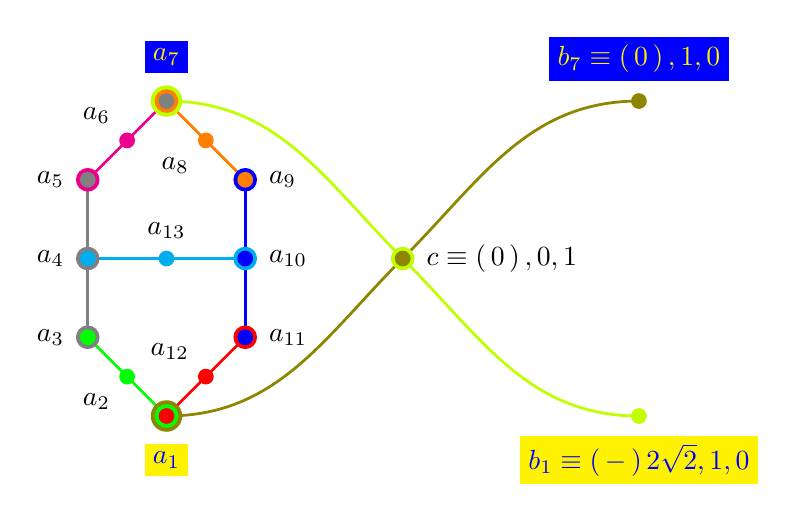
\begin{tikzpicture}  [scale=1]

\tikzstyle{every path}=[line width=1pt]

\newdimen\ms
\ms=0.1cm
\tikzstyle{s1}=[color=red,rectangle,inner sep=3.5]
\tikzstyle{c3}=[circle,inner sep={\ms/8},minimum size=4*\ms]
\tikzstyle{c2}=[circle,inner sep={\ms/8},minimum size=3*\ms]
\tikzstyle{c1}=[circle,inner sep={\ms/8},minimum size=2*\ms]

% Define positions of all observables

% bug #1
\coordinate (a1) at  (1,2);
\coordinate (a2) at (1.5,{(1-(1-0.5)/2)*2});
\coordinate (a3) at (2,1);
\coordinate (a4) at (2,0);
\coordinate (a5) at (2,-1);
\coordinate (a6) at (1.5,{(-0.5-(1-0.5)/2)*2});
\coordinate (a7) at (1,-2);
\coordinate (a8) at (0.5,{(-0.5-(1-0.5)/2)*2});
\coordinate (a9) at (0,-1);
\coordinate (a10) at (0,0);
\coordinate (a11) at (0,1);
\coordinate (a12) at (0.5,{(1-(1-0.5)/2)*2});
\coordinate (a13) at (1,0);

\coordinate (a14) at (4,0);

% bug #2
\coordinate (a21) at  ({6+1},2);
%\coordinate (a22) at ({6+1.5},{(1-(1-0.5)/2)*2});
%\coordinate (a23) at ({6+2},1);
%\coordinate (a24) at ({6+2},0);
%\coordinate (a25) at ({6+2},-1);
%\coordinate (a26) at ({6+1.5},{(-0.5-(1-0.5)/2)*2});
\coordinate (a27) at ({6+1},-2);
%\coordinate (a28) at ({6+0.5},{(-0.5-(1-0.5)/2)*2});
%\coordinate (a29) at ({6+0},-1);
%\coordinate (a210) at ({6+0},0);
%\coordinate (a211) at ({6+0},1);
%\coordinate (a212) at ({6+0}.5,{(1-(1-0.5)/2)*2});
%\coordinate (a213) at ({6+1},0);


% draw contexts

% bug #1
\draw [color=orange] (a1) -- (a3);
\draw [color=blue] (a3) -- (a5);
\draw [color=red] (a5) -- (a7);
\draw [color=green] (a7) -- (a9);
\draw [color=gray] (a9) -- (a11);
\draw [color=magenta] (a11) -- (a1);
\draw [color=cyan] (a10) -- (a4);

\draw [color=lime] (a1) to [out=0,in={90+45}] (a14) to [out={180+90+45},in=180]  (a27);
\draw [color=olive] (a7) to [out=0,in={180+45}] (a14) to [out=45,in=180] (a21);

% bug #2
%\draw [color=orange] (a21) -- (a23);
%\draw [color=blue] (a23) -- (a25);
%\draw [color=red] (a25) -- (a27);
%\draw [color=green] (a27) -- (a29);
%\draw [color=gray] (a29) -- (a211);
%\draw [color=magenta] (a211) -- (a21);
%\draw [color=cyan] (a210) -- (2a4);



% draw atoms

% bug 1
\draw (a1) coordinate[c3,fill=lime,label=above:{\colorbox{blue}{\textcolor{yellow}{$a_7$}}}];
\draw (a1) coordinate[c2,fill=orange];
\draw (a1) coordinate[c1,fill=gray];

\draw (a2) coordinate[c1,fill=orange,label=below left:$a_8$];

\draw (a3) coordinate[c2,fill=blue,label=right:$a_9$];
\draw (a3) coordinate[c1,fill=orange];

\draw (a4) coordinate[c2,fill=cyan,label=right:$a_{10}$];
\draw (a4) coordinate[c1,fill=blue];

\draw (a5) coordinate[c2,fill=red,label=right:$a_{11}$];
\draw (a5) coordinate[c1,fill=blue];

\draw (a6) coordinate[c1,fill=red,label=above left:$a_{12}$];

\draw (a7) coordinate[c3,fill=olive,label=below:{\colorbox{yellow}{\textcolor{blue}{$a_1$}}}];
\draw (a7) coordinate[c2,fill=green];
\draw (a7) coordinate[c1,fill=red];

\draw (a8) coordinate[c1,fill=green,label=below left:$a_2$];

\draw (a9) coordinate[c2,fill=gray,label=left:$a_3$];
\draw (a9) coordinate[c1,fill=green];

\draw (a10) coordinate[c2,fill=gray,label=left:$a_4$];
\draw (a10) coordinate[c1,fill=cyan];

\draw (a11) coordinate[c2,fill=magenta,label=left:$a_5$];
\draw (a11) coordinate[c1,fill=gray];

\draw (a12) coordinate[c1,fill=magenta,label=above left:$a_6$];

\draw (a13) coordinate[c1,fill=cyan,label=above:$a_{13}$];


\draw (a14) coordinate[c2,fill=lime,label=right:{$c \equiv \begin{pmatrix}0,0,1\end{pmatrix}$}];
\draw (a14) coordinate[c1,fill=olive];

\draw (a21) coordinate[c1,fill=olive,label=above:{\colorbox{blue}{\textcolor{yellow}{$b_7 \equiv \begin{pmatrix}0,1,0\end{pmatrix}$}}}];

\draw (a27) coordinate[c1,fill=lime,label=below:{\colorbox{yellow}{\textcolor{blue}{$b_1 \equiv \begin{pmatrix}-2\sqrt{2},1,0\end{pmatrix}$}}}];

% bug 2
%\draw (a21) coordinate[c2,fill=orange!20!white,label=above:$b_7$];
%\draw (a21) coordinate[c1,fill=gray!20!white];
%
%\draw (a22) coordinate[c1,fill=orange!20!white,label=below left:$b_8$];
%
%\draw (a23) coordinate[c2,fill=blue!20!white,label=right:$b_9$];
%\draw (a23) coordinate[c1,fill=orange!20!white];
%
%\draw (a24) coordinate[c2,fill=cyan!20!white,label=right:$b_{10}$];
%\draw (a24) coordinate[c1,fill=blue!20!white];
%
%\draw (a25) coordinate[c2,fill=red!20!white,label=right:$b_{11}$];
%\draw (a25) coordinate[c1,fill=blue!20!white];
%
%\draw (a26) coordinate[c1,fill=red!20!white,label=above left:$b_{12}$];
%
%\draw (a27) coordinate[c2,fill=green!20!white,label=below:$b_1$];
%\draw (a27) coordinate[c1,fill=red!20!white];
%
%\draw (a28) coordinate[c1,fill=green!20!white,label=below left:$b_2$];
%
%\draw (a29) coordinate[c2,fill=gray!20!white,label=left:$b_3$];
%\draw (a29) coordinate[c1,fill=green!20!white];
%
%\draw (a210) coordinate[c2,fill=gray!20!white,label=left:$b_4$];
%\draw (a210) coordinate[c1,fill=cyan!20!white];
%
%\draw (a211) coordinate[c2,fill=magenta!20!white,label=left:$b_5$];
%\draw (a211) coordinate[c1,fill=gray!20!white];
%
%\draw (a212) coordinate[c1,fill=magenta!20!white,label=above left:$b_6$];
%
%\draw (a213) coordinate[c1,fill=cyan!20!white,label=above:$b_{13}$];




\end{tikzpicture}
}
\end{center}
{\scriptsize
If $a_1$ is true (has value 1) then $b_1$ has to be true (has value 1).
Likewise,
if $a_7$ is true (has value 1) then $b_7$ has to be true (has value 1).
Just as for the Specker bug, a proof is either direct by enumerating all two-valued states (Travis matrix), or by contradiction.

Kochen {\&} Specker used an faithful orthogonal representation
allowing a serial composition of several TIT gadgets---actually, five TIT gadgets with
``aperture'', that is, angle between terminal points $a_1$ and $b_1$ or  $a_7$ and $b_7$
of $\frac{\pi}{10}$ or $\left(\frac{90}{5}\right)^\circ=18^\circ$---to arrive at a compound TIT gadget with ``aperture''
$\frac{\pi}{2}$ or $90^\circ$, which is forbidden, as it is within a new context.
}
\end{frame}

%%%%%%%%%%%%%%%%%%%%%%%%%%%%%%%%%%%%%%%%%%%%%%%%%%%%%%%%%%%%%%%%%%%%%%%%%%%%%%%%%%%%%%%%%%%%%%%%%%%%%%%%%%%%%%%%%%

\subsection{Extending two intertwining true-implies-true gadgets to a combo realizing classical propositional inseparability
and non-embeddability}

\begin{frame}%[shrink=2]
\frametitle{Extending two intertwining TIT gadgets to a combo realizing classical propositional inseparability
and non-embeddability}

From Kochen {\&} Specker, 1967,  DOI \href{https://doi.org/10.1512/iumj.1968.17.17004}{10.1512/iumj.1968.17.17004}

\begin{center}
\resizebox{0.6\textwidth}{!}{
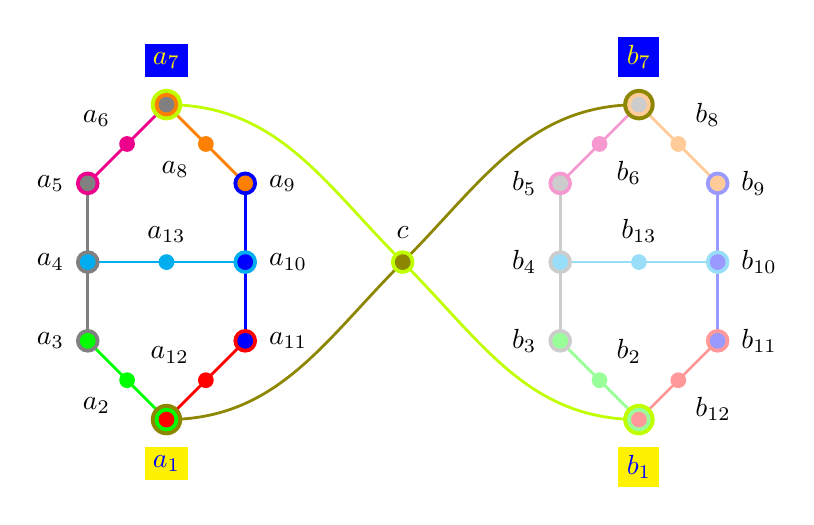
\begin{tikzpicture}  [scale=1]

\tikzstyle{every path}=[line width=1pt]

\newdimen\ms
\ms=0.1cm
\tikzstyle{s1}=[color=red,rectangle,inner sep=3.5]
\tikzstyle{c3}=[circle,inner sep={\ms/8},minimum size=4*\ms]
\tikzstyle{c2}=[circle,inner sep={\ms/8},minimum size=3*\ms]
\tikzstyle{c1}=[circle,inner sep={\ms/8},minimum size=2*\ms]

% Define positions of all observables

% bug #1
\coordinate (a1) at  (1,2);
\coordinate (a2) at (1.5,{(1-(1-0.5)/2)*2});
\coordinate (a3) at (2,1);
\coordinate (a4) at (2,0);
\coordinate (a5) at (2,-1);
\coordinate (a6) at (1.5,{(-0.5-(1-0.5)/2)*2});
\coordinate (a7) at (1,-2);
\coordinate (a8) at (0.5,{(-0.5-(1-0.5)/2)*2});
\coordinate (a9) at (0,-1);
\coordinate (a10) at (0,0);
\coordinate (a11) at (0,1);
\coordinate (a12) at (0.5,{(1-(1-0.5)/2)*2});
\coordinate (a13) at (1,0);

\coordinate (a14) at (4,0);

% bug #2
\coordinate (a21) at  ({6+1},2);
\coordinate (a22) at ({6+1.5},{(1-(1-0.5)/2)*2});
\coordinate (a23) at ({6+2},1);
\coordinate (a24) at ({6+2},0);
\coordinate (a25) at ({6+2},-1);
\coordinate (a26) at ({6+1.5},{(-0.5-(1-0.5)/2)*2});
\coordinate (a27) at ({6+1},-2);
\coordinate (a28) at ({6+0.5},{(-0.5-(1-0.5)/2)*2});
\coordinate (a29) at ({6+0},-1);
\coordinate (a210) at ({6+0},0);
\coordinate (a211) at ({6+0},1);
\coordinate (a212) at ({6+0.5},{(1-(1-0.5)/2)*2});
\coordinate (a213) at ({6+1},0);


% draw contexts

% bug #1
\draw [color=orange] (a1) -- (a3);
\draw [color=blue] (a3) -- (a5);
\draw [color=red] (a5) -- (a7);
\draw [color=green] (a7) -- (a9);
\draw [color=gray] (a9) -- (a11);
\draw [color=magenta] (a11) -- (a1);
\draw [color=cyan] (a10) -- (a4);

\draw [color=lime] (a1) to [out=0,in={90+45}] (a14) to [out={180+90+45},in=180]  (a27);
\draw [color=olive] (a7) to [out=0,in={180+45}] (a14) to [out=45,in=180] (a21);

% bug #2
\draw [color=orange!40!white] (a21) -- (a23);
\draw [color=blue!40!white] (a23) -- (a25);
\draw [color=red!40!white] (a25) -- (a27);
\draw [color=green!40!white] (a27) -- (a29);
\draw [color=gray!40!white] (a29) -- (a211);
\draw [color=magenta!40!white] (a211) -- (a21);
\draw [color=cyan!40!white] (a210) -- (a24);



% draw atoms

% bug 1
\draw (a1) coordinate[c3,fill=lime,label=above:{\colorbox{blue}{\textcolor{yellow}{$a_7$}}}];
\draw (a1) coordinate[c2,fill=orange];
\draw (a1) coordinate[c1,fill=gray];

\draw (a2) coordinate[c1,fill=orange,label=below left:$a_8$];

\draw (a3) coordinate[c2,fill=blue,label=right:$a_9$];
\draw (a3) coordinate[c1,fill=orange];

\draw (a4) coordinate[c2,fill=cyan,label=right:$a_{10}$];
\draw (a4) coordinate[c1,fill=blue];

\draw (a5) coordinate[c2,fill=red,label=right:$a_{11}$];
\draw (a5) coordinate[c1,fill=blue];

\draw (a6) coordinate[c1,fill=red,label=above left:$a_{12}$];

\draw (a7) coordinate[c3,fill=olive,label=below:{\colorbox{yellow}{\textcolor{blue}{$a_1$}}}];
\draw (a7) coordinate[c2,fill=green];
\draw (a7) coordinate[c1,fill=red];

\draw (a8) coordinate[c1,fill=green,label=below left:$a_2$];

\draw (a9) coordinate[c2,fill=gray,label=left:$a_3$];
\draw (a9) coordinate[c1,fill=green];

\draw (a10) coordinate[c2,fill=gray,label=left:$a_4$];
\draw (a10) coordinate[c1,fill=cyan];

\draw (a11) coordinate[c2,fill=magenta,label=left:$a_5$];
\draw (a11) coordinate[c1,fill=gray];

\draw (a12) coordinate[c1,fill=magenta,label=above left:$a_6$];

\draw (a13) coordinate[c1,fill=cyan,label=above:$a_{13}$];


\draw (a14) coordinate[c2,fill=lime,label=above:{$c$}];
\draw (a14) coordinate[c1,fill=olive];

\draw (a21) coordinate[c3,fill=olive,label=above:{\colorbox{blue}{\textcolor{yellow}{$b_7$}}}];

\draw (a27) coordinate[c3,fill=lime,label=below:{\colorbox{yellow}{\textcolor{blue}{$b_1$}}}];

% bug 2
\draw (a21) coordinate[c2,fill=orange!40!white];
\draw (a21) coordinate[c1,fill=gray!40!white];

\draw (a22) coordinate[c1,fill=orange!40!white,label=above right:$b_8$];

\draw (a23) coordinate[c2,fill=blue!40!white,label=right:$b_9$];
\draw (a23) coordinate[c1,fill=orange!40!white];

\draw (a24) coordinate[c2,fill=cyan!40!white,label=right:$b_{10}$];
\draw (a24) coordinate[c1,fill=blue!40!white];

\draw (a25) coordinate[c2,fill=red!40!white,label=right:$b_{11}$];
\draw (a25) coordinate[c1,fill=blue!40!white];

\draw (a26) coordinate[c1,fill=red!40!white,label=below right:$b_{12}$];

\draw (a27) coordinate[c2,fill=green!40!white];
\draw (a27) coordinate[c1,fill=red!40!white];

\draw (a28) coordinate[c1,fill=green!40!white,label=above right:$b_2$];

\draw (a29) coordinate[c2,fill=gray!40!white,label=left:$b_3$];
\draw (a29) coordinate[c1,fill=green!40!white];

\draw (a210) coordinate[c2,fill=gray!40!white,label=left:$b_4$];
\draw (a210) coordinate[c1,fill=cyan!40!white];

\draw (a211) coordinate[c2,fill=magenta!40!white,label=left:$b_5$];
\draw (a211) coordinate[c1,fill=gray!40!white];

\draw (a212) coordinate[c1,fill=magenta!40!white,label=below right:$b_6$];

\draw (a213) coordinate[c1,fill=cyan!40!white,label=above:$b_{13}$];


\end{tikzpicture}
}
\end{center}
{\scriptsize
If $a_1$ is true (has value 1) then $b_1$ has to be true (has value 1), and vice versa.
Likewise,
if $a_7$ is true (has value 1) then $b_7$ has to be true (has value 1), and vice versa.
Therefore,
$a_1$ cannot be classically separated from  $b_1$, and
$a_7$ cannot be classically separated from  $b_7$.
Just as for the Specker bug, a proof is either direct by enumerating all two-valued states (Travis matrix), or by contradiction.
Non-embedability follows from non-separability, see
Kochen {\&} Specker's Theorem~0.
}
\end{frame}


%%%%%%%%%%%%%%%%%%%%%%%%%%%%%%%%%%%%%%%%%%%%%%%%%%%%%%%%%%%%%%%%%%%%%%%%%%%%%%%%%%%%%%%%%%%%%%%%%%%%%%%%%%%%%%%%%%


\subsection{A true-implies-false gadget and a true-implies-true gadget with identical terminal points}

\begin{frame}%[shrink=2]
\frametitle{A true-implies-false gadget and a true-implies-true gadget with identical terminal points}

DOI \href{https://doi.org/10.3390/e20060406}{10.3390/e20060406}
based on
Abbott, Calude, and KS DOI \href{https://doi.org/10.1063/1.4931658}{10.1063/1.4931658}


\begin{center}
\resizebox{0.8\textwidth}{!}{
\begin{tabular}{cc}
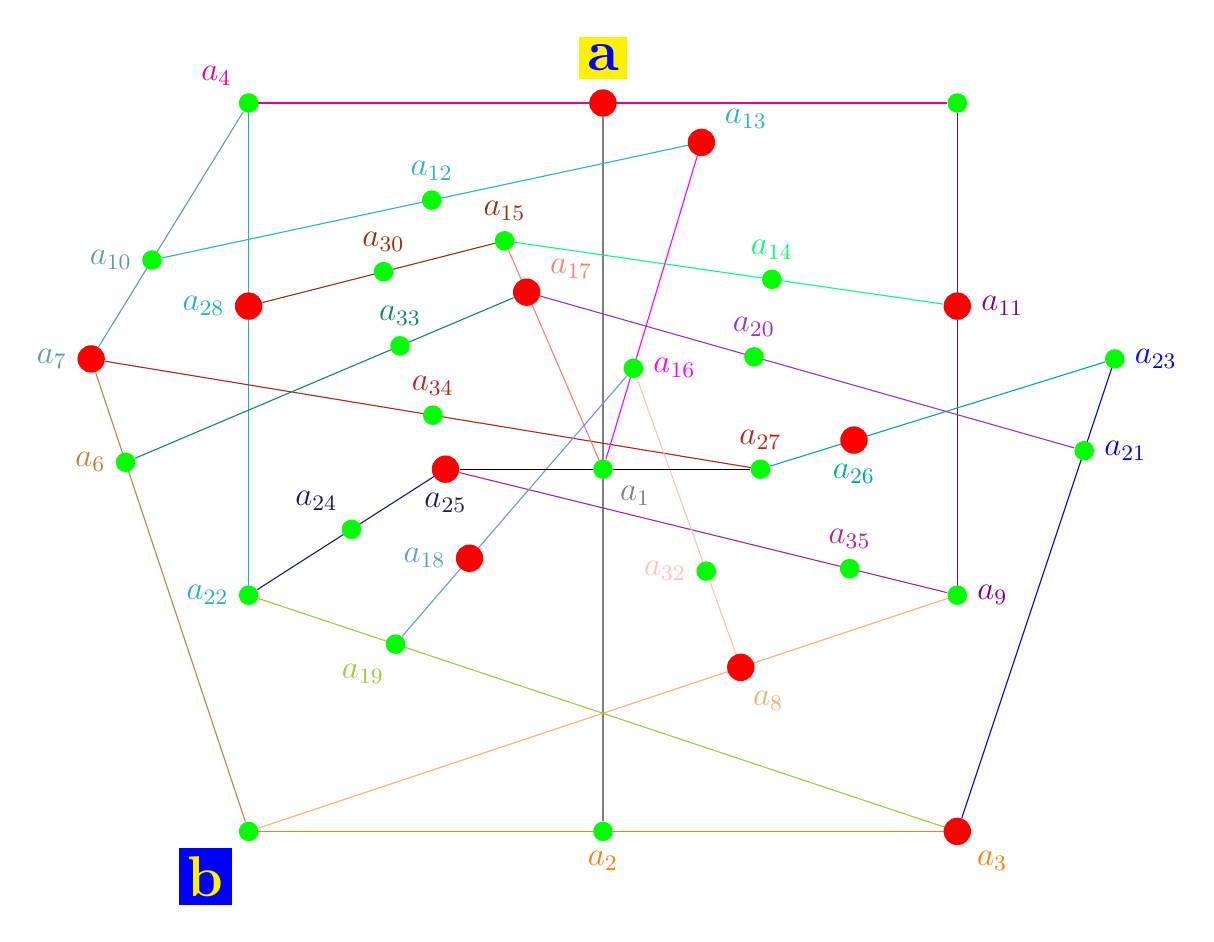
\begin{tikzpicture} [scale=0.5,rotate=0]
   %\tikzstyle{every path}=[line width=1.5pt]
   \tikzstyle{c1}=[color=green,circle,inner sep=2.5]
   \tikzstyle{s1}=[color=red,circle,inner sep=3.5]
   \tikzstyle{l1}=[draw=none,circle,minimum size=4]

   % Define positions of all observables

\draw [color=orange] (4,0) coordinate[c1,fill,label=225:{\colorbox{blue}{\textcolor{yellow}{\huge ${\bf b}$}}}] (b) -- (13,0)  coordinate[c1,fill,label=270:{ \large $a_2$}] (2) -- (22,0) coordinate[s1,fill,label=315:{ \large $a_3$}] (3);
\draw [color=blue, ] (3) -- (26,12) coordinate[c1,fill,pos=0.8,label=0:{ \large $a_{21}$}] (21) coordinate[c1,fill,label=0:{ \large $a_{23}$}] (23);
\draw [color=white] (23) -- (22,18.5) coordinate[c1,fill,pos=0.4,color=white,label=0:{ \large $a_{29}$}] (29) coordinate[c1,fill,label=45:{ \large $a_5$}] (5);
\draw [color=magenta,] (5)-- (13,18.5)coordinate[s1,fill,label=90:{\colorbox{yellow}{\textcolor{blue}{\huge ${\bf a}$}}}] (a) -- (4,18.5) coordinate[c1,fill,label=135:{ \large $a_4$}] (4);
\draw [color=CadetBlue, ] (4) -- (0,12) coordinate[c1,fill,pos=0.6,label=180:{ \large $a_{10}$}] (10) coordinate[s1,fill,label=180:{ \large $a_7$}] (7);
\draw [color=brown, ](7) -- (b)   coordinate[c1,fill,pos=0.2,label=180:{ \large $a_6$}] (6);

   \draw [color=gray] (a) -- (2) coordinate[c1,fill,pos=0.5,label=315:{ \large $a_1$}] (1);

   \draw [color=violet] (5) -- (22,6) coordinate[s1,fill,pos=0.4,label=0:{ \large $a_{11}$}] (11) coordinate[c1,fill,label=0:{ \large $a_9$}] (9);

\draw [color=Apricot] (9) -- (b) coordinate[s1,fill,pos=0.3,label=280:{ \large $a_8$}] (8);

\draw [color=TealBlue] (4) -- (4,6) coordinate[s1,fill,pos=0.4,label=180:{ \large $a_{28}$}] (28) coordinate[c1,fill,label=180:{ \large $a_{22}$}] (22);
\draw [color=YellowGreen] (22) -- (3) coordinate[c1,fill,pos=0.2,label=260:{ \large $a_{19}$}] (19);

   \coordinate (25) at ([xshift=-4cm]1);
   \coordinate (27) at ([xshift=4cm]1);

\draw [color=MidnightBlue] (22) -- (25) coordinate[c1,fill,pos=0.5,label=115:{ \large $a_{24}$}] (24) coordinate[s1,fill,label=270:{ \large $a_{25}$}] (25);
\draw [color=Mulberry] (25) -- (9) coordinate[c1,fill,pos=0.8,label=90:{ \large $a_{35}$}] (35);

\draw [color=BrickRed] (7) -- (27) coordinate[c1,fill,pos=0.5,label=90:{ \large $a_{34}$}] (34) coordinate[c1,fill,label=90:{ \large $a_{27}$}] (27);
\draw [color=Emerald] (27) -- (23) coordinate[s1,fill,pos=0.25,label=270:{ \large $a_{26}$}] (26);

\draw [color=BlueGreen] (10) -- (15.5,17.5) coordinate[c1,fill,pos=0.5,label=90:{ \large $a_{12}$}] (12) coordinate[s1,fill,label=15:{ \large $a_{13}$}] (13);
%\draw [color=Tan] (13) -- (29) coordinate[c1,fill,pos=0.4,label=90:{ \large $a_{31}$}] (31);

\draw [color=RawSienna] (28) -- (10.5,15) coordinate[c1,fill,pos=0.5,label=90:{ \large $a_{30}$}] (30) coordinate[c1,fill,label=90:{ \large $a_{15}$}] (15);
\draw [color=SpringGreen] (15) -- (11) coordinate[c1,fill,pos=0.6,label=90:{ \large $a_{14}$}] (14);

\draw [color=Salmon] (15) -- (1) coordinate[s1,fill,pos=0.2,label=15:{ \large $a_{17}$}] (17);
\draw [color=Fuchsia] (1)-- (13) coordinate[c1,fill,pos=0.3,label=0:{ \large $a_{16}$}] (16);

\draw [color=CornflowerBlue] (19) -- (16) coordinate[s1,fill,pos=0.3,label=180:{ \large $a_{18}$}] (18);
\draw [color=pink] (16) -- (8) coordinate[c1,fill,pos=0.7,label=180:{ \large $a_{32}$}] (32);

\draw [color=PineGreen] (6) -- (17) coordinate[c1,fill,pos=0.7,label=90:{ \large $a_{33}$}] (33);
\draw [color=DarkOrchid] (17) -- (21) coordinate[c1,fill,pos=0.4,label=90:{ \large $a_{20}$}] (20);

\draw [color=black] (25) -- (1) -- (27);

%\coordinate (ContextLabel) at ([shift=({-2cm,-3mm})]1);
%\draw (ContextLabel) coordinate[l1,label=90:{ \large $C_{26}$}];

\end{tikzpicture}
&
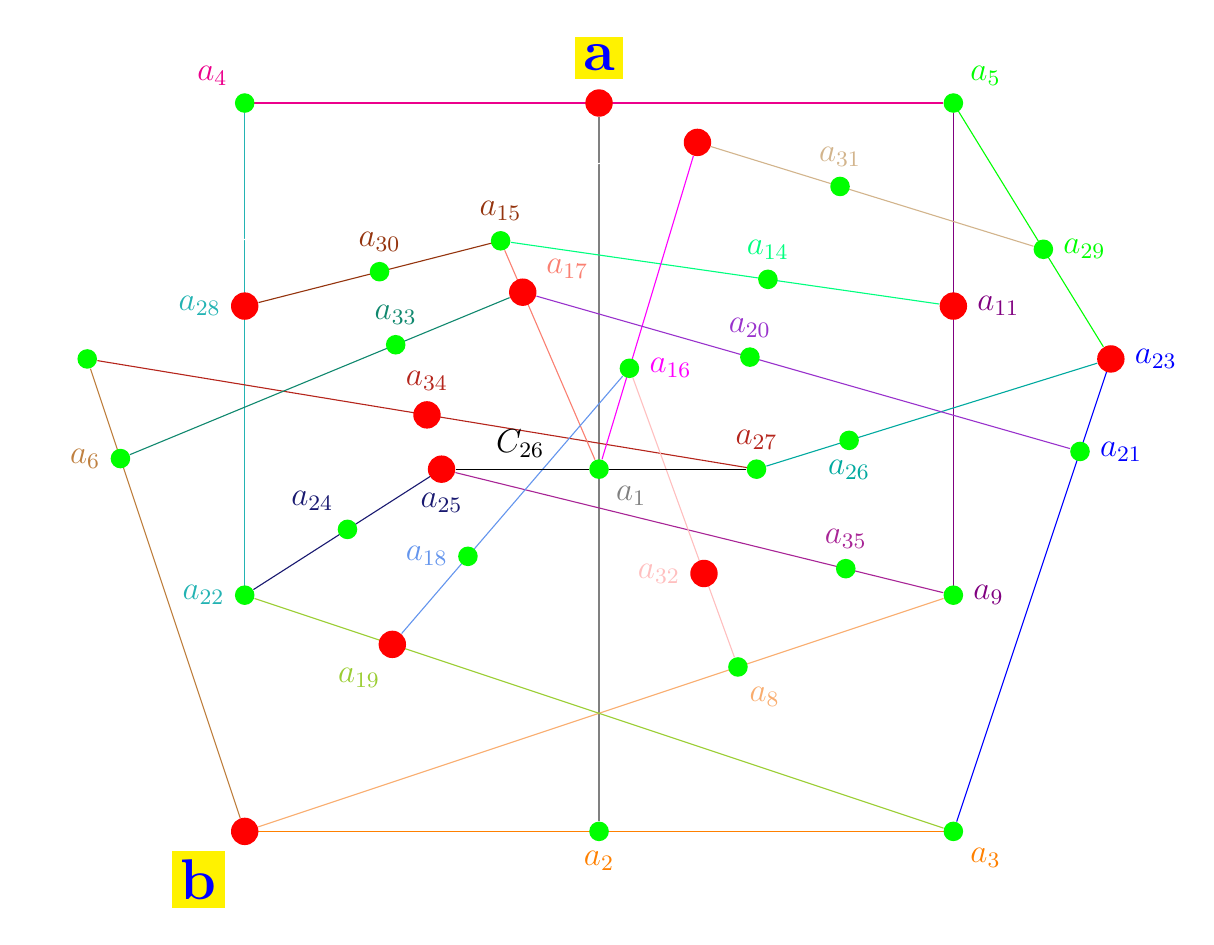
\begin{tikzpicture} [scale=0.5]
   %\tikzstyle{every path}=[line width=1.5pt]
   \tikzstyle{c1}=[color=green,circle,inner sep=2.5]
   \tikzstyle{s1}=[color=red,circle,inner sep=3.5]
   \tikzstyle{l1}=[draw=none,circle,minimum size=4]

   % Define positions of all observables

\draw [color=orange] (4,0) coordinate[s1,fill,label=225:{\colorbox{yellow}{\textcolor{blue}{\huge ${\bf b}$}}}] (b) -- (13,0)  coordinate[c1,fill,label=270:{ \large $a_2$}] (2) -- (22,0) coordinate[c1,fill,label=315:{ \large $a_3$}] (3);
\draw [color=blue, ] (3) -- (26,12) coordinate[c1,fill,pos=0.8,label=0:{ \large $a_{21}$}] (21) coordinate[s1,fill,label=0:{ \large $a_{23}$}] (23);
\draw [color=green] (23) -- (22,18.5) coordinate[c1,fill,pos=0.4,label=0:{ \large $a_{29}$}] (29) coordinate[c1,fill,label=45:{ \large $a_5$}] (5);
\draw [color=magenta,] (5)-- (13,18.5)coordinate[s1,fill,label=90:{\colorbox{yellow}{\textcolor{blue}{\huge ${\bf a}$}}}] (a) -- (4,18.5) coordinate[c1,fill,label=135:{ \large $a_4$}] (4);
\draw [color=white] (4) -- (0,12) coordinate[c1,color=white,fill,pos=0.6,label=180:{ \large $a_{10}$}] (10) coordinate[c1,fill,label=180:{ \large $a_7$}] (7);
\draw [color=brown, ] (7) -- (b)   coordinate[c1,fill,pos=0.2,label=180:{ \large $a_6$}] (6);

   \draw [color=gray] (a) -- (2) coordinate[c1,fill,pos=0.5,label=315:{ \large $a_1$}] (1);

   \draw [color=violet] (5) -- (22,6) coordinate[s1,fill,pos=0.4,label=0:{ \large $a_{11}$}] (11) coordinate[c1,fill,label=0:{ \large $a_9$}] (9);

\draw [color=Apricot] (9) -- (b) coordinate[c1,fill,pos=0.3,label=280:{ \large $a_8$}] (8);

\draw [color=TealBlue] (4) -- (4,6) coordinate[s1,fill,pos=0.4,label=180:{ \large $a_{28}$}] (28) coordinate[c1,fill,label=180:{ \large $a_{22}$}] (22);
\draw [color=YellowGreen] (22) -- (3) coordinate[s1,fill,pos=0.2,label=260:{ \large $a_{19}$}] (19);

   \coordinate (25) at ([xshift=-4cm]1);
   \coordinate (27) at ([xshift=4cm]1);

\draw [color=MidnightBlue] (22) -- (25) coordinate[c1,fill,pos=0.5,label=115:{ \large $a_{24}$}] (24) coordinate[s1,fill,label=270:{ \large $a_{25}$}] (25);
\draw [color=Mulberry] (25) -- (9) coordinate[c1,fill,pos=0.8,label=90:{ \large $a_{35}$}] (35);

%\draw [color=BrickRed] (7) -- (27) coordinate[c1,fill,pos=0.5,label=90:{ \large $a_{34}$}] (34) coordinate[c1,fill,label=90:{ \large $a_{27}$}] (27);
\draw [color=BrickRed] (7) -- (27) coordinate[s1,fill,pos=0.5,label=90:{ \large $a_{34}$}] (34) coordinate[c1,fill,label=90:{ \large $a_{27}$}] (27);
\draw [color=Emerald] (27) -- (23) coordinate[c1,fill,pos=0.25,label=270:{ \large $a_{26}$}] (26);

\draw [color=white] (10) -- (15.5,17.5) coordinate[c1,color=white,fill,pos=0.5,label=90:{ \large $a_{12}$}] (12) coordinate[s1,fill,label=15:{ \large $a_{13}$}] (13);
\draw [color=Tan] (13) -- (29) coordinate[c1,fill,pos=0.4,label=90:{ \large $a_{31}$}] (31);

\draw [color=RawSienna] (28) -- (10.5,15) coordinate[c1,fill,pos=0.5,label=90:{ \large $a_{30}$}] (30) coordinate[c1,fill,label=90:{ \large $a_{15}$}] (15);
\draw [color=SpringGreen] (15) -- (11) coordinate[c1,fill,pos=0.6,label=90:{ \large $a_{14}$}] (14);

\draw [color=Salmon] (15) -- (1) coordinate[s1,fill,pos=0.2,label=15:{ \large $a_{17}$}] (17);
\draw [color=Fuchsia] (1)-- (13) coordinate[c1,fill,pos=0.3,label=0:{ \large $a_{16}$}] (16);

\draw [color=CornflowerBlue] (19) -- (16) coordinate[c1,fill,pos=0.3,label=180:{ \large $a_{18}$}] (18);
\draw [color=pink] (16) -- (8) coordinate[s1,fill,pos=0.7,label=180:{ \large $a_{32}$}] (32);

\draw [color=PineGreen] (6) -- (17) coordinate[c1,fill,pos=0.7,label=90:{ \large $a_{33}$}] (33);
\draw [color=DarkOrchid] (17) -- (21) coordinate[c1,fill,pos=0.4,label=90:{ \large $a_{20}$}] (20);

\draw [color=black] (25) -- (1) -- (27);

   \coordinate (ContextLabel) at ([shift=({-2cm,-3mm})]1);
   \draw (ContextLabel) coordinate[l1,label=90:{ \large $C_{26}$}];

   \end{tikzpicture}
\\
TIF gadget & TIT gadget
\end{tabular}
}
\end{center}

{\scriptsize
If $a$ is true (has value 1) then,
\begin{enumerate}
\item[ ]
according to the TIF gadget: $b$ cannot be true (cannot have value 1);
\item[ ]
according to the TIT gadget: $b$ cannot be false (cannot have value 0).
\end{enumerate}
Therefore,  if $a$ is true (has value 1), $b$ can neither be true nor false (has neither the values 0 nor 1):
it needs to be \textbf{value indefinite/indeterminate}.

See also Pitowsky
DOI \href{https://doi.org/10.1063/1.532334}{10.1063/1.532334}.
}


\end{frame}


%%%%%%%%%%%%%%%%%%%%%%%%%%%%%%%%%%%%%%%%%%%%%%%%%%%%%%%%%%%%%%%%%%%%%%%%%%%%%%%%%%%%%%%%%%%%%%%%%%%%%%%%%%%%%%%%%%


\subsection{Quantum propositional structures whose classical interpretation requires certain observables to be true and others false (nonunitality)}

\begin{frame}%[shrink=2]
\frametitle{Quantum propositional structures whose classical interpretation requires certain observables to be true and others false (nonunitality)}

DOI \href{https://doi.org/10.1007/978-3-030-34316-3\_24}{10.1007/978-3-030-34316-3\_24}
based on
Abbott, Calude, and KS DOI \href{https://doi.org/10.1063/1.4931658}{10.1063/1.4931658}

\resizebox{1\textwidth}{!}{
\begin{tabular}{cc}
\resizebox{0.45\textwidth}{!}{
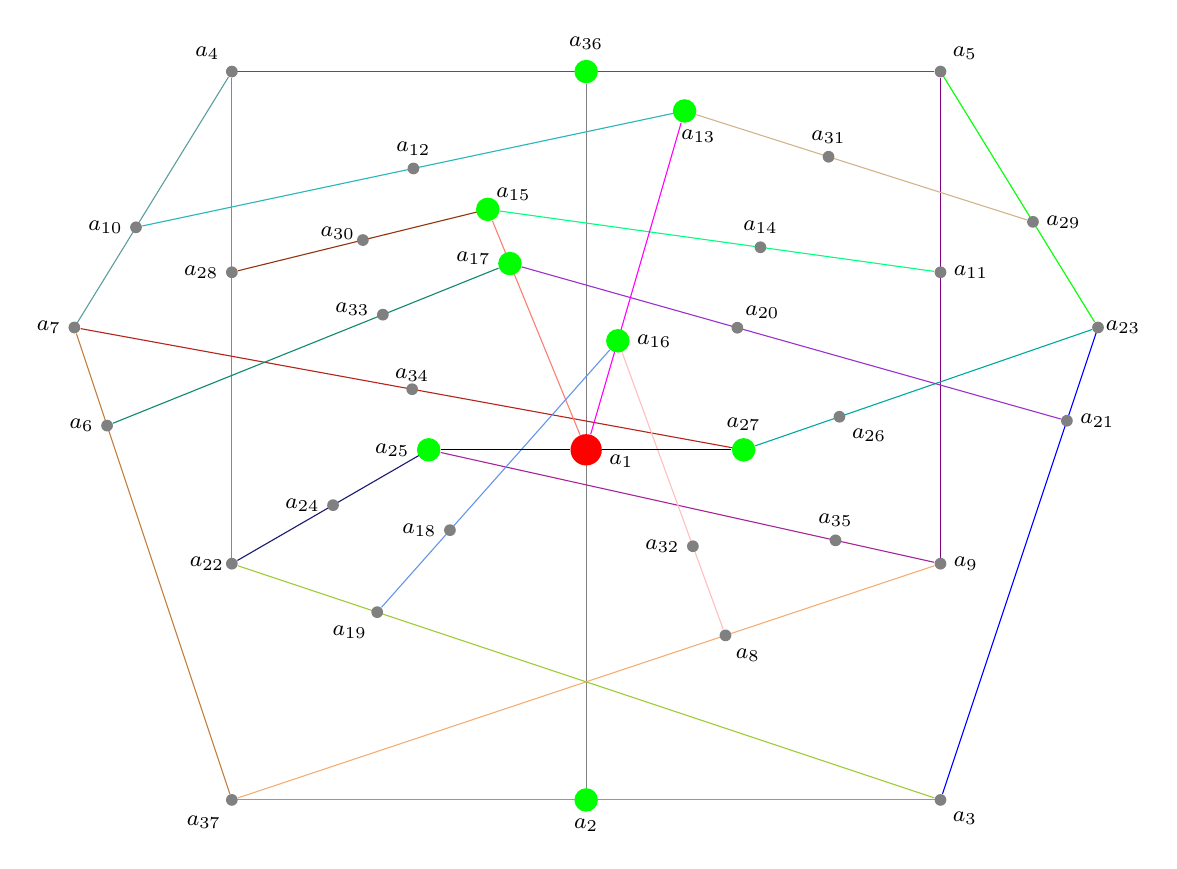
\begin{tikzpicture}  [scale=0.5, rotate=0]
        %\tikzstyle{every path}=[line width=1.5pt]
%\tikzstyle{c1}=[circle,fill,inner sep=4]
%\tikzstyle{c2}=[circle,fill,inner sep=2.7]
       \tikzstyle{c1}=[color=gray,circle,inner sep=1.5]
       \tikzstyle{c2}=[color=green,circle,inner sep=3]
        \tikzstyle{s1}=[color=red,circle,inner sep=4]
        \tikzstyle{l1}=[draw=none,circle,minimum size=6]

        % Define positions of all observables



\draw [color=orange]  (4,0)  coordinate[c1,fill,label=260:{\color{black}\footnotesize $a_{37}$}] (b) -- (13,0)    coordinate[c2,fill,label={[label distance=-1]270:{\footnotesize \color{black}  $a_2$}}] (2) -- (22,0)  coordinate[c1,fill,label={[label distance=-1]315:{\footnotesize \color{black}  $a_3$}}] (3);
\draw [color=blue] (3) -- (26,12)  coordinate[c1,fill,pos=0.8,label={[label distance=-1]0:{\footnotesize \color{black}  $a_{21}$}}] (21) coordinate[c1,fill,label={[label distance=-3]0:{\footnotesize \color{black}  $a_{23}$}}] (23);
\draw [color=green] (23) -- (22,18.5) coordinate[c1,fill,pos=0.4,label={[label distance=-1]0:{\footnotesize \color{black}  $a_{29}$}}] (29) coordinate[c1,fill,label={[label distance=-1]45:{\footnotesize \color{black}  $a_5$}}] (5);
\draw [color=magenta] (5)-- (13,18.5)coordinate[c2,fill,label=90:{\color{black}\footnotesize $a_{36}$}] (a) -- (4,18.5)  coordinate[c1,fill,label={[label distance=-1]135:{\footnotesize \color{black}  $a_4$}}] (4);
\draw [color=CadetBlue] (4) -- (0,12)   coordinate[c1,fill,pos=0.6,label={[label distance=-1]180:{\footnotesize \color{black}  $a_{10}$}}] (10)  coordinate[c1,fill,label={[label distance=-1]180:{\footnotesize \color{black}  $a_7$}}] (7);
\draw [color=brown] (7) -- (b)      coordinate[c1,fill,pos=0.2,label={[label distance=-1]180:{\footnotesize \color{black}  $a_6$}}] (6);






        \draw [color=gray] (a) -- (2) coordinate[s1,fill,pos=0.52,label={[label distance=-1, yshift=2]357.5:{\footnotesize \color{black}  $a_1$}}] (1);

        \draw [color=violet] (5) -- (22,6) coordinate[c1,fill,pos=0.4,label={[label distance=-1]0:{\footnotesize \color{black}  $a_{11}$}}] (11) coordinate[c1,fill,label={[label distance=-1]0:{\footnotesize \color{black}  $a_9$}}] (9);

\draw [color=Apricot] (9) -- (b) coordinate[c1,fill,pos=0.3,label={[label distance=-1]280:{\footnotesize \color{black}  $a_8$}}] (8);

\draw [color=TealBlue] (4) -- (4,6) coordinate[c1,fill,pos=0.4,label={[label distance=-1]180:{\footnotesize \color{black}  $a_{28}$}}] (28) coordinate[c1,fill,label={[label distance=-3]180:{\footnotesize \color{black}  $a_{22}$}}] (22);
\draw [color=YellowGreen] (22) -- (3) coordinate[c1,fill,pos=0.2,label={[label distance=-1]260:{\footnotesize \color{black}  $a_{19}$}}] (19);

        \coordinate (25) at ([xshift=-4cm]1);
        \coordinate (27) at ([xshift=4cm]1);

\draw [color=MidnightBlue]  (22) -- (25) coordinate[c1,fill,pos=0.5,label={[label distance=-1]180:{\footnotesize \color{black}  $a_{24}$}}] (24) coordinate[c2,fill,label={[label distance=-1]180:{\footnotesize \color{black}  $a_{25}$}}] (25);
\draw [color=Mulberry] (25) -- (9) coordinate[c1,fill,pos=0.8,label={[label distance=-1]90:{\footnotesize \color{black}  $a_{35}$}}] (35);

\draw [color=BrickRed]  (7) -- (27) coordinate[c1,fill,pos=0.5,label={[label distance=-3]90:{\footnotesize \color{black}  $a_{34}$}}] (34) coordinate[c2,fill,label={[label distance=-1]90:{\footnotesize \color{black}  $a_{27}$}}] (27);
\draw [color=Emerald] (27) -- (23) coordinate[c1,fill,pos=0.25,label={[label distance=-1]320:{\footnotesize \color{black}  $a_{26}$}}] (26);

\draw [color=BlueGreen]  (10) -- (15.5,17.5) coordinate[c1,fill,pos=0.5,label={[label distance=-1]90:{\footnotesize \color{black}  $a_{12}$}}] (12) coordinate[c2,fill,label={[label distance=-1,xshift=5]270:{\footnotesize \color{black}  $a_{13}$}}] (13);
\draw [color=Tan] (13) -- (29) coordinate[c1,fill,pos=0.4,label={[label distance=-1]90:{\footnotesize \color{black}  $a_{31}$}}] (31);

\draw [color=RawSienna]  (28) -- (10.5,15) coordinate[c1,fill,pos=0.5,label={[label distance=-3, yshift=-3]160:{\footnotesize \color{black}  $a_{30}$}}] (30) coordinate[c2,fill,label={[label distance=-5]45:{\footnotesize \color{black}  $a_{15}$}}] (15);
\draw [color=SpringGreen] (15) -- (11) coordinate[c1,fill,pos=0.6,label={[label distance=-1]90:{\footnotesize \color{black}  $a_{14}$}}] (14);

\draw [color=Salmon]  (15) -- (1) coordinate[c2,fill,pos=0.2,label={[label distance=-1, yshift=2]180:{\footnotesize \color{black}  $a_{17}$}}] (17);
\draw [color=Fuchsia] (1)-- (13) coordinate[c2,fill,pos=0.3,label={[label distance=-1]0:{\footnotesize \color{black}  $a_{16}$}}] (16);

\draw [color=CornflowerBlue]  (19) -- (16) coordinate[c1,fill,pos=0.3,label={[label distance=-1]180:{\footnotesize \color{black}  $a_{18}$}}] (18);
\draw [color=pink] (16) -- (8) coordinate[c1,fill,pos=0.7,label={[label distance=-1]180:{\footnotesize \color{black}  $a_{32}$}}] (32);

\draw [color=PineGreen]  (6) -- (17) coordinate[c1,fill,pos=0.7,label={[label distance=-1, yshift=2]180:{\footnotesize \color{black}  $a_{33}$}}] (33);
\draw [color=DarkOrchid] (17) -- (21) coordinate[c1,fill,pos=0.4,label={[label distance=-3]20:{\footnotesize \color{black}  $a_{20}$}}] (20);

\draw [color=black] (25) -- (1) -- (27);

\end{tikzpicture}
}
&
\setcounter{MaxMatrixCols}{40}
\raisebox{2.0cm}{
\resizebox{0.6\textwidth}{!}{
$
\begin{pmatrix}
&\cellcolor{red!10}{\color{red}1}&\cellcolor{green!10}{\color{green}0}& 0& 1& 0& 0& 0& 0& 0& 0& 1& 1&\cellcolor{green!10}{\color{green}0}& 0&\cellcolor{green!10}{\color{green}0}&\cellcolor{green!10}{\color{green}0}&\cellcolor{green!10}{\color{green}0}& 0& 1& 0& 1& 0& 0& 1&\cellcolor{green!10}{\color{green}0}& 1&\cellcolor{green!10}{\color{green}0}& 0& 1& 1& 0& 1& 1& 1& 1&\cellcolor{green!10}{\color{green}0}& 1&\\
&\cellcolor{red!10}{\color{red}1}&\cellcolor{green!10}{\color{green}0}& 0& 1& 0& 0& 0& 0& 0& 0& 1& 1&\cellcolor{green!10}{\color{green}0}& 0&\cellcolor{green!10}{\color{green}0}&\cellcolor{green!10}{\color{green}0}&\cellcolor{green!10}{\color{green}0}& 0& 1& 1& 0& 0& 1& 1&\cellcolor{green!10}{\color{green}0}& 0&\cellcolor{green!10}{\color{green}0}& 0& 0& 1& 1& 1& 1& 1& 1&\cellcolor{green!10}{\color{green}0}& 1&\\
&\cellcolor{red!10}{\color{red}1}&\cellcolor{green!10}{\color{green}0}& 0& 0& 1& 0& 0& 0& 0& 1& 0& 0&\cellcolor{green!10}{\color{green}0}& 1&\cellcolor{green!10}{\color{green}0}&\cellcolor{green!10}{\color{green}0}&\cellcolor{green!10}{\color{green}0}& 0& 1& 0& 1& 0& 0& 1&\cellcolor{green!10}{\color{green}0}& 1&\cellcolor{green!10}{\color{green}0}& 1& 0& 0& 1& 1& 1& 1& 1&\cellcolor{green!10}{\color{green}0}& 1&\\
&\cellcolor{red!10}{\color{red}1}&\cellcolor{green!10}{\color{green}0}& 0& 0& 1& 0& 0& 0& 0& 1& 0& 0&\cellcolor{green!10}{\color{green}0}& 1&\cellcolor{green!10}{\color{green}0}&\cellcolor{green!10}{\color{green}0}&\cellcolor{green!10}{\color{green}0}& 1& 0& 0& 1& 1& 0& 0&\cellcolor{green!10}{\color{green}0}& 1&\cellcolor{green!10}{\color{green}0}& 0& 0& 1& 1& 1& 1& 1& 1&\cellcolor{green!10}{\color{green}0}& 1&\\
&\cellcolor{red!10}{\color{red}1}&\cellcolor{green!10}{\color{green}0}& 1& 1& 0& 1& 0& 1& 0& 0& 1& 1&\cellcolor{green!10}{\color{green}0}& 0&\cellcolor{green!10}{\color{green}0}&\cellcolor{green!10}{\color{green}0}&\cellcolor{green!10}{\color{green}0}& 1& 0& 1& 0& 0& 0& 1&\cellcolor{green!10}{\color{green}0}& 1&\cellcolor{green!10}{\color{green}0}& 0& 1& 1& 0& 0& 0& 1& 1&\cellcolor{green!10}{\color{green}0}& 0&\\
&\cellcolor{red!10}{\color{red}1}&\cellcolor{green!10}{\color{green}0}& 1& 1& 0& 1& 0& 0& 1& 0& 0& 1&\cellcolor{green!10}{\color{green}0}& 1&\cellcolor{green!10}{\color{green}0}&\cellcolor{green!10}{\color{green}0}&\cellcolor{green!10}{\color{green}0}& 1& 0& 1& 0& 0& 0& 1&\cellcolor{green!10}{\color{green}0}& 1&\cellcolor{green!10}{\color{green}0}& 0& 1& 1& 0& 1& 0& 1& 0&\cellcolor{green!10}{\color{green}0}& 0&\\
&\cellcolor{red!10}{\color{red}1}&\cellcolor{green!10}{\color{green}0}& 1& 0& 1& 1& 0& 1& 0& 1& 0& 0&\cellcolor{green!10}{\color{green}0}& 1&\cellcolor{green!10}{\color{green}0}&\cellcolor{green!10}{\color{green}0}&\cellcolor{green!10}{\color{green}0}& 1& 0& 1& 0& 0& 0& 1&\cellcolor{green!10}{\color{green}0}& 1&\cellcolor{green!10}{\color{green}0}& 1& 0& 0& 1& 0& 0& 1& 1&\cellcolor{green!10}{\color{green}0}& 0&\\
&\cellcolor{red!10}{\color{red}1}&\cellcolor{green!10}{\color{green}0}& 1& 0& 1& 0& 1& 1& 0& 0& 0& 1&\cellcolor{green!10}{\color{green}0}& 1&\cellcolor{green!10}{\color{green}0}&\cellcolor{green!10}{\color{green}0}&\cellcolor{green!10}{\color{green}0}& 1& 0& 1& 0& 0& 0& 1&\cellcolor{green!10}{\color{green}0}& 1&\cellcolor{green!10}{\color{green}0}& 1& 0& 0& 1& 0& 1& 0& 1&\cellcolor{green!10}{\color{green}0}& 0&\\
\end{pmatrix}$
}
}
\end{tabular}
}


Proposition $a_1$ must be true (value 1) all the time.

Propositions $a_2,a_{13}, a_{15}, a_{16},a_{17},a_{25},a_{27},a_{36}$ must be false (value 0) all the time.

Note: one can always change the coordinate system / basis and rotate a state or a dichotomic elementary proposition into $a_1$ or $a_2$.

What does such an outcome signify? Cf.
DOI \href{https://doi.org/10.3390/quantum2020018}{10.3390/quantum2020018}

\end{frame}

%%%%%%%%%%%%%%%%%%%%%%%%%%%%%%%%%%%%%%%%%%%%%%%%%%%%%%%%%%%%%%%%%%%%%%%%%%%%%%%%%%%%%%%%%%%%%%%%%%%%%%%%%%%%%%%%%%


\begin{frame}%[shrink=2]
\frametitle{Quantum propositional structures whose classical interpretation
requires certain observables to be true and others false (nonunitality) cntd.}

The configuration of observables, if interpreted classically,
forces one observable to be true all the time and thus some adjacent, connected ones to be false all the time.

In operational terms this is equivalent of stating that the classical prediction is that no observable can be prepared to be in any of its two particular states: it can neither be true nor false, because depending on one value I can always rotate my basis such that my state coincides with the ``one'' or ``zero'' value states, respectively.

This, in my opinion, may well be the eclipse---or the end---of this kind of graph-theoretic considerations in quantum mechanics: one can derive an immediate, almost trivially testable, contradiction relative to the assumption of classical value definiteness.


\end{frame}

%\subsection{Ten tightly bi-intertwining contexts with three mutually exclusive observables (Greechie's $G_{32}$ hypergraph)}


\frame{

\centerline{\Large {\color{magenta} Thank you for your attention!}}

\begin{center}\color{orange}
$\widetilde{\qquad \qquad }$
$\widetilde{\qquad \qquad}$
$\widetilde{\qquad \qquad }$
\end{center}
 }


 \end{document}

%%%%%%%%%%%%%%%%%%%%%%%%%%%%%%%%%%%%%%%%%%%%%%%%%%%%%%%%%%%%%%%%

import cdd

mat = cdd.Matrix([
[ 1, 1 , 0 ],
[ 1, 0,  1 ]
])
poly = cdd.Polyhedron(mat)
ine = poly.get_inequalities()
print(ine)

%%%%%%%%%%%%%%%%%%%%%%%%%%%%%%%%%%%%%%%%%%%%%%%%%%%%%%%%%%%%%%%%

import cdd

mat = cdd.Matrix([
[ 1, 1 , 0 , 0 , 0 ],
[ 1, 0,  1 , 0 , 0 ],
[ 1, 0,  0 , 1 , 0 ],
[ 1, 0,  0 , 0 , 1 ]
])
poly = cdd.Polyhedron(mat)
ine = poly.get_inequalities()
print(ine)

%%%%%%%%%%%%%%%%%%%%%%%%%%%%%%%%%%%%%%%%%%%%%%%%%%%%%%%%%%%%%%%%

import cdd

mat = cdd.Matrix([
[ 1, 0 , 0, 0 ],
[ 1, 0 , 1, 0 ],
[ 1, 1 , 0, 0 ],
[ 1, 1 , 1, 1 ]
])
poly = cdd.Polyhedron(mat)
ine = poly.get_inequalities()
print(ine)

%%%%%%%%%%%%%%%%%%%%%%%%%%%%%%%%%%%%%%%%%%%%%%%%%%%%%%%%%%%%%%%%

import cdd

mat = cdd.Matrix([
[ 1, -1 , -1, 1 ],
[ 1, -1 , 1, -1 ],
[ 1, 1 , -1, -1 ],
[ 1, 1 , 1, 1 ]
])
poly = cdd.Polyhedron(mat)
ine = poly.get_inequalities()
print(ine)

% SZ %%%%%%%%%%%%%%%%%%%%%%%%%%%%%%%%%%%%%%%%%%%%%%%%%%%%%%%%%%%%%%%

import cdd

mat = cdd.Matrix([
[1, 1 , 1 , 1 ],
[1, 1 , -1 , -1 ],
[1, -1 , 1 , -1 ],
[1, -1 , -1 , 1 ]])
poly = cdd.Polyhedron(mat)
ine = poly.get_inequalities()
print(ine)

% CHSH %%%%%%%%%%%%%%%%%%%%%%%%%%%%%%%%%%%%%%%%%%%%%%%%%%%%%%%%%%%%%%%

import cdd

mat = cdd.Matrix([
[1, 1, 1, 1, 1],
[1, 1,-1, 1,-1],
[1,-1, 1,-1, 1],
[1,-1,-1,-1,-1],
[1, 1, 1,-1,-1],
[1, 1,-1,-1, 1],
[1,-1, 1, 1,-1],
[1,-1,-1, 1, 1]])
poly = cdd.Polyhedron(mat)
ine = poly.get_inequalities()
print(ine)

% firefly: 2 x 3 %%%%%%%%%%%%%%%%%%%%%%%%%%%%%%%%%%%%%%%%%%%%%%%%%%%%%%%%%%%%%%%

import cdd

mat = cdd.Matrix([
[1, 1, 0, 0, 1, 0, 1, 0, 0, 0],
[1, 1, 0, 0, 0, 1, 0, 1, 0, 0],
[1, 0, 1, 0, 1, 0, 0, 0, 1, 0],
[1, 0, 1, 0, 0, 1, 0, 0, 0, 1],
[1, 0, 0, 1, 0, 0, 0, 0, 0, 0]])
poly = cdd.Polyhedron(mat)
ine = poly.get_inequalities()
print(ine)



import cdd

mat = cdd.Matrix([
[1,   1, -1, -1,  1, -1,  1, -1, -1,  1 ],
[1,   1, -1, -1, -1,  1, -1,  1,  1, -1 ],
[1,  -1,  1, -1,  1, -1, -1,  1,  1, -1 ],
[1,  -1,  1, -1, -1,  1,  1, -1, -1,  1 ],
[1,  -1, -1,  1, -1, -1,  1,  1,  1,  1 ]])
poly = cdd.Polyhedron(mat)
ine = poly.get_inequalities()
print(ine)


################################################################

rot=RotationTransform[{{Sqrt[2],-1,0},{1,0,0}}]

m = TransformationMatrix[rot];
(* FullSimplify[m[[1 ;; 3, 1 ;; 3]]] *)
mi = Inverse[TransformationMatrix[rot]];  (* inverse *)

FullSimplify[mi[[1 ;; 3, 1 ;; 3]].{1,0,0}] (* check with inverse *)

a1 = {1,0,0};

a7 =  FullSimplify[m[[1 ;; 3, 1 ;; 3]].{Sqrt[2],1,0}];

a3 =  {1,Sqrt[2],1};
a4 =  {1,0,-1};
a5 =  {-1,Sqrt[2],-1};


Print["a3 ",FullSimplify[m[[1 ;; 3, 1 ;; 3]].a3]]
Print["a4 ",FullSimplify[m[[1 ;; 3, 1 ;; 3]].a4]]
Print["a5 ",FullSimplify[m[[1 ;; 3, 1 ;; 3]].a5]]

a11 = {1,Sqrt[2],-1};
a10 = {1,0,1};
a9 = {-1,Sqrt[2],1};

Print["a11 ",FullSimplify[m[[1 ;; 3, 1 ;; 3]].a11]]
Print["a10 ",FullSimplify[m[[1 ;; 3, 1 ;; 3]].a10]]
Print["a9 ",FullSimplify[m[[1 ;; 3, 1 ;; 3]].a9]]

Print["a13 ",Cross[FullSimplify[m[[1 ;; 3, 1 ;; 3]].a4] ,FullSimplify[m[[1 ;; 3, 1 ;; 3]].a10] ]](* a13 *)
Print["a2 ",Cross[a1 ,FullSimplify[m[[1 ;; 3, 1 ;; 3]].a3 ]]](* a2 *)
Print["a12 ",Cross[a1 ,FullSimplify[m[[1 ;; 3, 1 ;; 3]].a11] ]](* a12 *)
Print["a6 ",Cross[FullSimplify[m[[1 ;; 3, 1 ;; 3]].a5] ,a7 ]](* a6 *)
Print["a8 ",Cross[FullSimplify[m[[1 ;; 3, 1 ;; 3]].a9] ,a7 ]](* a8 *)


Print["c ",FullSimplify[m[[1 ;; 3, 1 ;; 3]].{0,0,1} ]](* c *)
Print["b1 ",FullSimplify[m[[1 ;; 3, 1 ;; 3]].{-1,Sqrt[2],0} ]](* b1 *)
Print["b7 ",FullSimplify[m[[1 ;; 3, 1 ;; 3]].{1,Sqrt[2],0} ]](* b7 *)
